\documentclass[12pt, draftcls, onecolumn]{IEEEtran}

\usepackage{bm}
\usepackage{verbatim}
\usepackage{algorithm}
\usepackage{soul,xcolor}
\usepackage[T1]{fontenc}
\usepackage{algcompatible}
\usepackage[normalem]{ulem}
\usepackage{multirow,enumitem}

\usepackage{url}
\usepackage{bbm}
\usepackage{cite}
\usepackage{array}
\usepackage{ifthen}
\usepackage{xspace}
\usepackage{dsfont}
\usepackage{epsfig}
\usepackage{caption}
\usepackage{amsmath}
\usepackage{amssymb}
\usepackage{multicol}
\usepackage{amsfonts}
\usepackage{mathrsfs}
\usepackage{booktabs}
\usepackage{epstopdf}
\usepackage{graphicx}
\usepackage{subcaption}
\usepackage{algpseudocode}

\usepackage{esint}
\usepackage{amsthm}
\usepackage{cancel}
\usepackage{siunitx}
\usepackage{setspace}
\usepackage{hyperref}
\usepackage{makecell}
\usepackage{footnote}

\captionsetup{font=small}
\captionsetup[sub]{font=footnotesize}

\renewcommand\qedsymbol{$\blacksquare$}

\renewcommand\theadalign{c}
\renewcommand\theadfont{\bfseries}
\renewcommand\cellgape{\Gape[2pt]}
\renewcommand\theadgape{\Gape[2pt]}

\theoremstyle{plain}
\newtheorem{lemma}{Lemma}
\newtheorem{theorem}{Theorem}

\theoremstyle{definition}
\newtheorem{defi}{Definition}
\newtheorem{corollary}{Corollary}

\theoremstyle{remark}
\newtheorem{remark}{Remark}
\newtheorem{nota}{Notation}

\newcommand{\tot}{\mathrm{tot}}
\newcommand{\numberthis}{\addtocounter{equation}{1}\tag{\theequation}}

\sisetup{detect-all,range-phrase=--,range-units=single}
\newcommand\mst[2][red]{\setbox0=\hbox{$#2$}\rlap{\raisebox{.45\ht0}{\textcolor{#1}{\rule{\wd0}{2pt}}}}#2}

\newcommand{\bk}[1]{\textcolor{blue}{[BK: #1]}}
\newcommand{\mb}[1]{\textcolor{blue}{[MB: #1]}}
\newcommand{\nm}[1]{\textcolor{magenta}{[NM: #1]}}

\newcommand{\sst}[1]{\st{#1}}
\newcommand{\prob}{\mathbb{P}}
\newcommand{\tfr}{T_{\mathrm{fr}}}
\newcommand{\vect}[1]{\mathbf{#1}}
\newcommand{\wtot}{W_{\mathrm{tot}}}
\newcommand{\add}[1]{\textcolor{red}{#1}}

\DeclareMathOperator{\Exp}{\mathbb{E}}
\DeclareMathOperator*{\argmax}{arg\,max}
\DeclareMathOperator*{\argmin}{arg\,min}

\newcommand{\tfrm}{T_{\mathrm{fr}}}
\newcommand{\beam}[1]{\mathcal B_{#1}}
\newcommand{\size}[1]{\left | #1 \right|}
\newcommand{\beambs}[1]{\mathcal B_{{\mathrm t},#1}}
\newcommand{\beamue}[1]{\mathcal B_{{\mathrm r},#1}}
\newcommand{\diag}[1]{\mathrm{diag}\left(#1 \right)}


\title{MAESTRO-X: Distributed Orchestration of Rotary-Wing UAV Relay Swarms via SMDPs}
\author{Bharath Keshavamurthy\IEEEauthorrefmark{1}, Matthew Bliss\IEEEauthorrefmark{2}, and Nicol\`{o} Michelusi\IEEEauthorrefmark{1}
\thanks{Part of this work has been supported by NSF under grants CNS-1642982 and CNS-2129015.}
\thanks{\IEEEauthorrefmark{1}Electrical, Computer and Energy Engineering, Arizona State University, Tempe, AZ.}
\thanks{\IEEEauthorrefmark{2}Electrical and Computer Engineering, Purdue University, West Lafayette, IN.}
\thanks{A preliminary version of this manuscript appeared at IEEE ICC 2020 \cite{ICC}.}
\thanks{The source code for this project is available on \href{https://github.com/bharathkeshavamurthy/Aesir.git}{GitHub} \cite{Aesir}.}
\vspace{-6mm}
}


\begin{document}
\maketitle
\thispagestyle{plain}
\pagestyle{plain}
\setulcolor{red}
\setul{red}{2pt}
\setstcolor{red}
\vspace{-14mm}


\begin{abstract}
In this work, we detail the design of a scalable framework to orchestrate a swarm of rotary-wing Unmanned Aerial Vehicles (UAVs) serving as cellular relays to facilitate beyond line-of-sight connectivity and traffic offloading for ground users, thereby enhancing the coverage and service capabilities of the constituent terrestrial base station. First, restricting our deployment model to a single relay, we develop MAESTRO, a Multiscale Adaptive Energy-conscious Scheduling and TRajectory Optimization framework, whose goal is to minimize the time-average service delay of ground users, subject to an average UAV power constraint. Formulated as a semi-Markov decision process and equipped with rate adaptation to efficiently exploit air-to-ground channel conditions, we prove that the underlying objective imbibes a multiscale structure to our model and its resultant solution: outer actions involving radial wait velocities and final service positions are established via value iteration to optimize the long-term delay-power trade-off; consequently, inner actions are selected to determine power-minimizing angular wait velocities and service trajectories that minimize an instantaneous delay-power cost metric via hierarchical competitive swarm optimization. Next, this single-agent construction is eXtended to UAV swarms (MAESTRO-X) by replicating the optimal single-relay policy across the swarm, augmented with spread maximization, M/G/x queueing dynamics, and consensus-driven conflict resolution. Numerical evaluations demonstrate that MAESTRO-X significantly improves scalability and performance vis-à-vis average service times and average per-UAV power consumption: simulating a swarm of $3$ UAVs, MAESTRO-X delivers the data payload $4\times$ faster than Q-learning, $6\times$ faster than successive convex approximation, and $10\times$ faster than alternating direction method-of-multipliers. Finally, through emulations employing the radio and vehicle control software of the NSF AERPAW platform, we prove the integration and implementation feasibility of our framework.
\end{abstract}
\vspace{-4mm}


\begin{IEEEkeywords}
Unmanned Aerial Vehicles, Markov Decision Processes, Competitive Swarm Optimization
\end{IEEEkeywords}
\vspace{-4mm}


\section{Introduction}\label{S1}
\vspace{-2mm}

With sustained device proliferation, enterprises across sectors have stepped-up their adoption of unmanned aerial vehicles\footnote{These are also referred to as drones, unmanned aerial systems, and autonomous aerial relays.} to gather data, survey infrastructure, monitor operations, and automate logistics \cite{UAVSurvey, UAVTutorial}. Inevitably, this has fostered varied academic research and industrial R\&D on drone-augmented beyond line-of-sight connectivity and traffic offloading in cellular networks: the coverage and service capabilities of an extant terrestrial radio access network\footnote{This can either be a single base station or a K-tier heterogeneous network of several base stations.} are enhanced by the mobility and maneuverability of these autonomous aerial relays \cite{LOSDominance, FundamentalTradeoffs}. 

These assets of drone-assisted networks are especially obvious in military environments, public safety scenarios, disaster-relief applications, and mechanized farming. Our prior work on cognitive communications \cite{TCCN} involved performance analyses and mobility studies of an intelligent spectrum sensing and access framework, applied to emulated military scenarios constituting troop deployments accompanied by unmanned aerial relays (e.g., Alleys of Austin scenario evaluations in the DARPA Spectrum Collaboration Challenge \cite{Alleys-of-Austin}). $5$G-enabled autonomous drones have facilitated near real-time high-definition video streaming of potential public-safety risks, thereby allowing state and local agencies to effectively monitor and deploy resources to handle these emerging situations with less risk \cite{VerizonPublicSafety}. When the existing wireless infrastructure was rendered inaccessible during the Big Hollow fire in Washington state, Verizon's fleet of LTE-enabled drones allowed for efficient and expedient deployments of robust air-to-ground links to relay real-time imagery to an operations base several miles away \cite{VerizonDisasterRelief}. Recent innovations in sensor manufacturing and virtualization platforms have resulted in their widespread expansion into precision agriculture: unmanned aerial systems serve as additive companions to MooCall livestock monitoring sensors, AgOpenGPS seeding workflows, and VIGOR soil-moisture sensing platforms \cite{VerizonAgriculture}. Fig. \ref{F1} depicts a typical deployment seen in mechanized farms and ranches, where a swarm of UAVs support traffic offloading for cellular devices and extend coverage for precision agricultural sensors.

\begin{figure} [t]
    \centering
    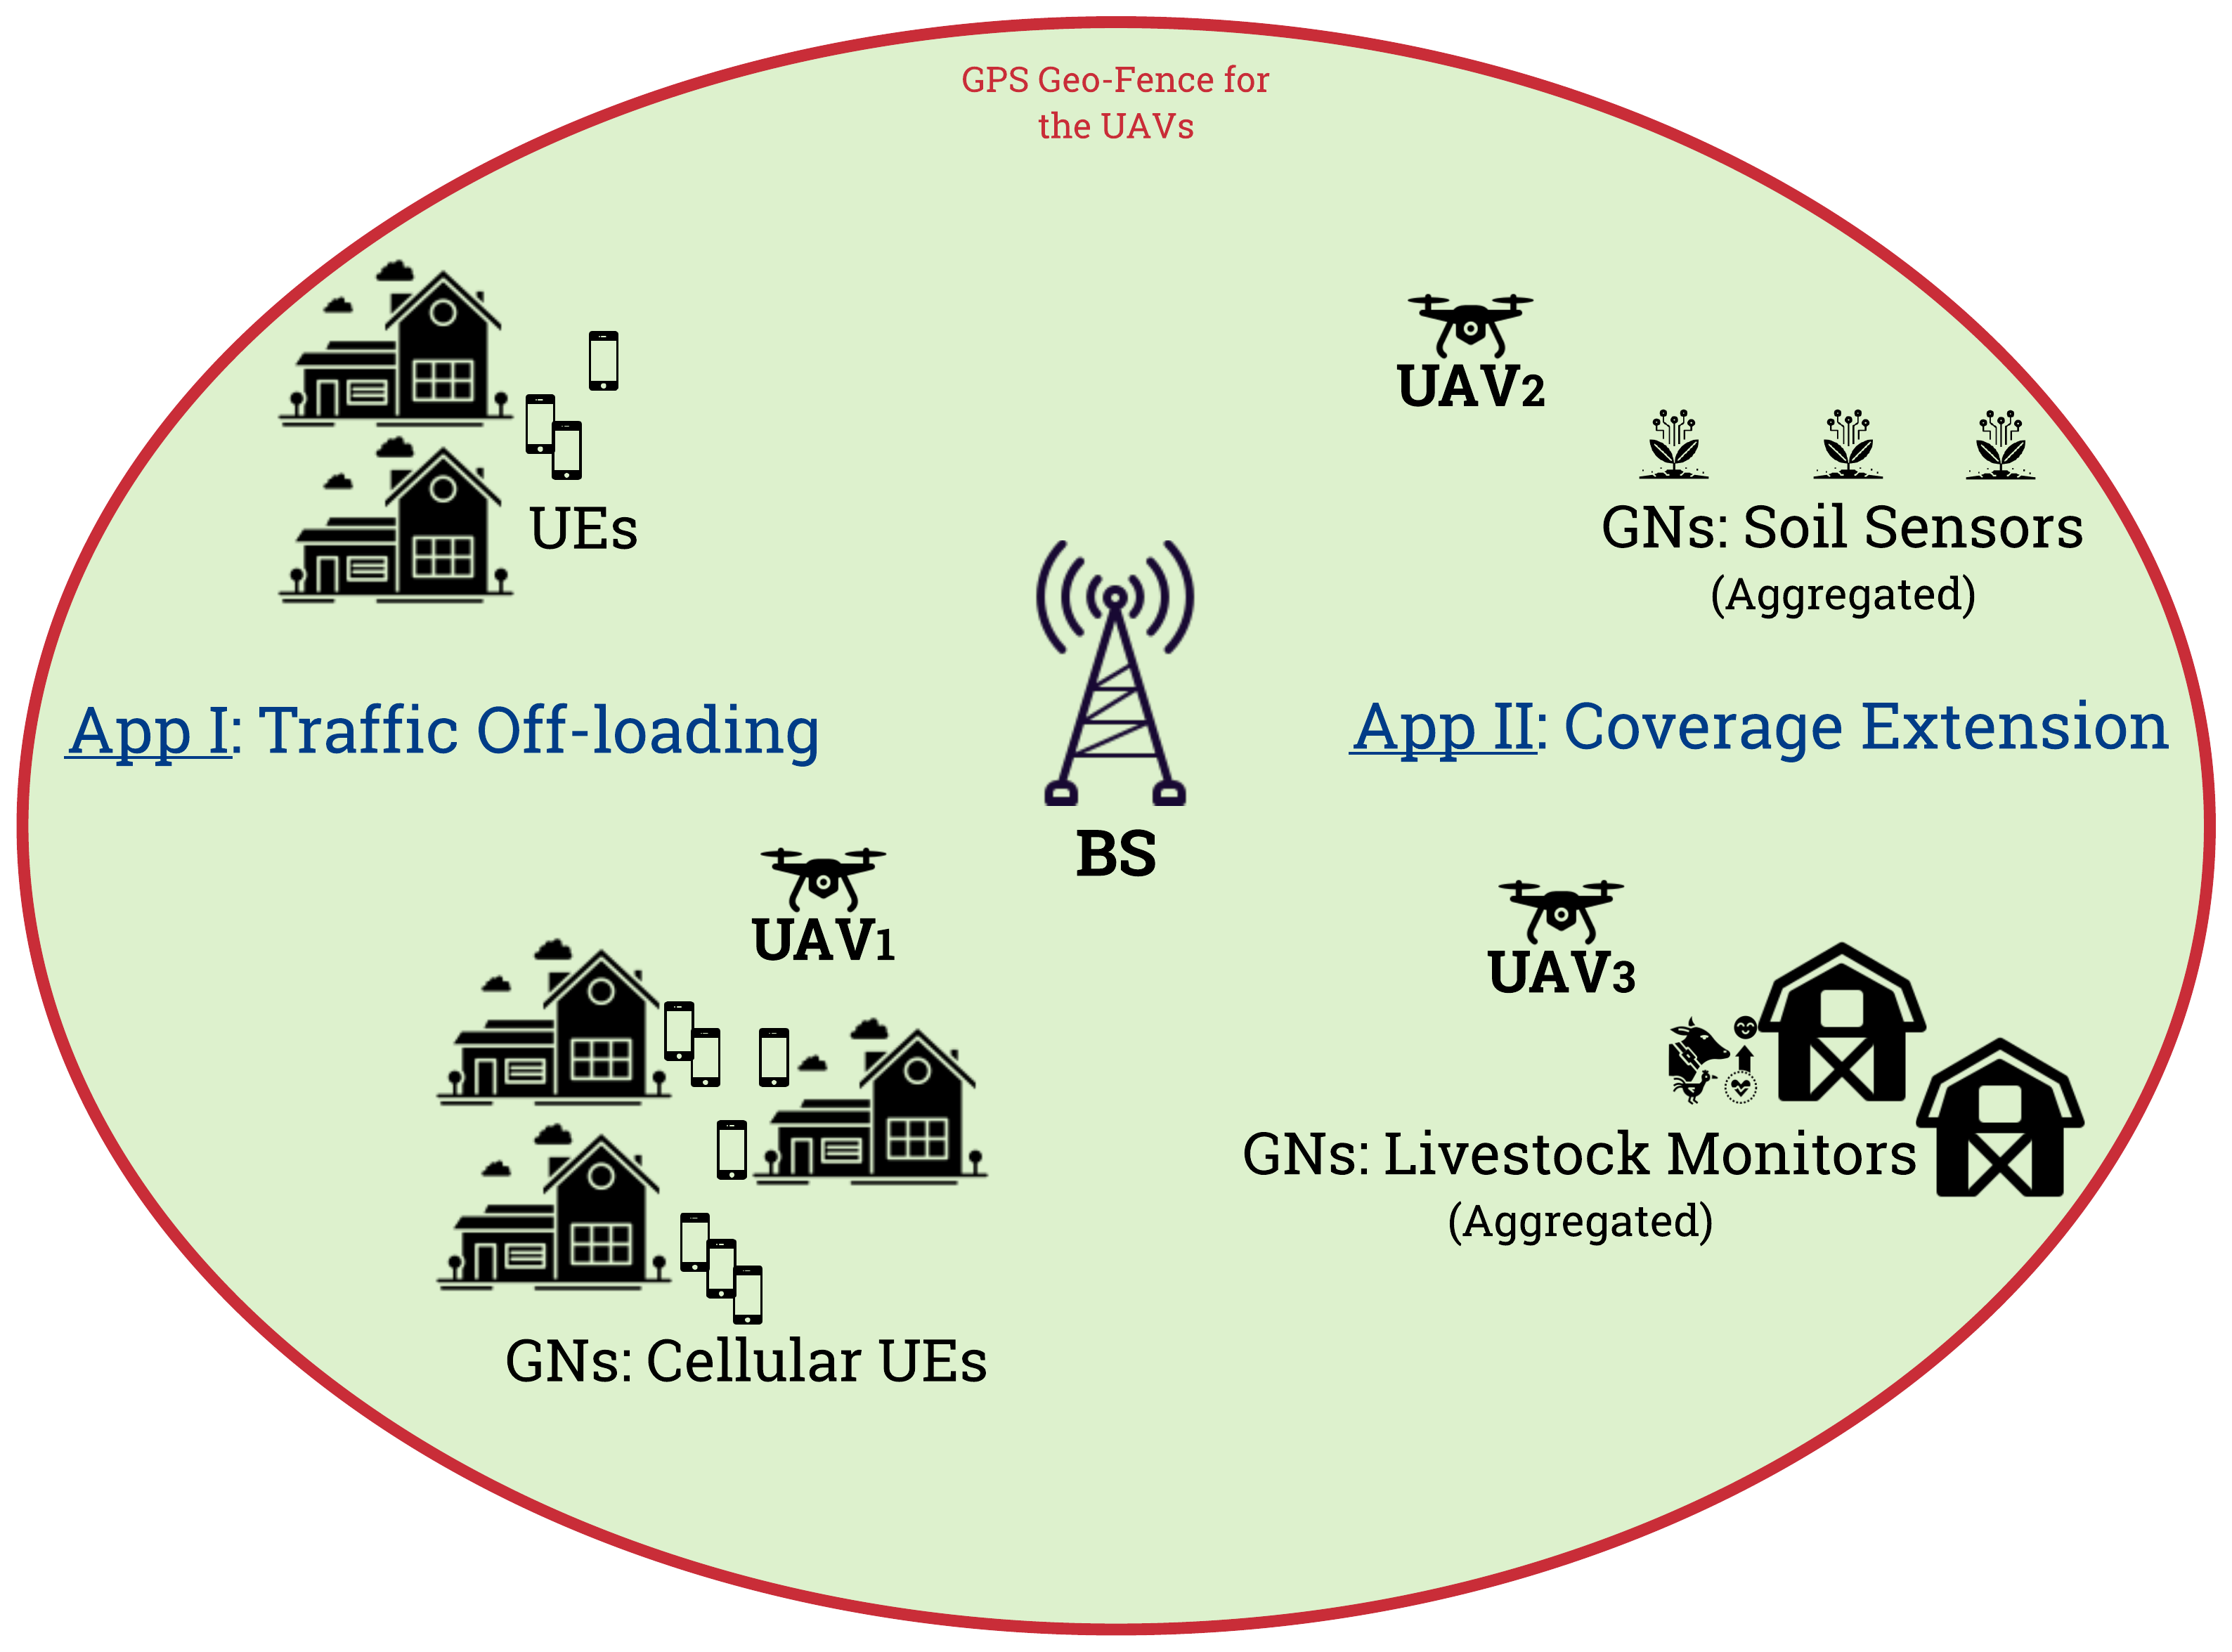
\includegraphics[width=0.7\linewidth]{figs/System_Architecture_I.png}
    \caption{\emph{(Not to scale)} A terrestrial Base Station (BS) aided by a swarm of $3$ Unmanned Aerial Vehicles (UAVs) serving as wireless relays for a diverse set of Ground Nodes (GNs): traffic offloading for cellular User Equipment (UEs) and coverage extensions for livestock monitors and soil sensors. The GPS geo-fence ensures bounded operations of the UAVs.}
    \vspace{-10mm}
    \label{F1}
\end{figure}

Unsurprisingly, the pervasive potential of such hybrid wireless networks brings along a plethora of challenges in real-world deployments \cite{FundamentalTradeoffs}: specifically, on-board energy constraints of aerial platforms impacting mission times, stringent Quality-of-Service (QoS) requirements for accessible and reliable connectivity, channel stochastics of air-to-ground links in highly-mobile settings, and computational feasibility challenges in trajectory design brought on by the inherently large state and action spaces. Ergo, several works in the state-of-the-art have tried to tackle these challenges using tools from convex optimization, machine learning, and reinforcement learning---however, various problems remain unsolved and various challenges are left unaddressed. 

Recognizing the need to abridge this wide-gap between conceptualization and implementation, we consider a distributed deployment where multiple power-constrained Unmanned Aerial Vehicles (UAVs), equipped with transceiver chains, supplement a terrestrial Base Station (BS) by relaying dynamically-generated data traffic from a random distribution of Ground Nodes (GNs). Coupled with rate adaptation to leverage Air-to-Ground (A2G) propagation conditions, management of queueing dynamics, computing accelerations, and consensus-driven decentralized operations, the proposals detailed in our work constitute a scalable framework to efficiently automate a swarm of UAV relays.

\noindent{\textbf{Novelties}}: Constructing a realistic channel model that accounts for A2G channel characteristics in highly-mobile settings, we propose a computationally efficient method for rate adaptation that optimizes throughput by leveraging large-scale path-loss conditions and small-scale fading statistics. Initially, we constrain our study to a single UAV relay by proposing the Multiscale Adaptive Energy-conscious Scheduling and TRajectory Optimization (MAESTRO) framework. In particular, with the underlying objective of minimizing the time-average communication service delay subject to an average UAV mobility power constraint, we formulate the problem as a Semi-Markov Decision Process (SMDP). Considering the UAV's operations in both its waiting and communication states, this formulation and its resultant solution exhibit a multiscale structure, i.e., minimizing the long-term delay-power costs yields outer decisions on radial wait velocities and service positions (via value iteration); next, given these outer decisions, greedily minimizing the instantaneous delay-power costs yields inner actions on angular wait velocities (via exhaustive search) and service trajectories (via hierarchical competitive swarm optimization). In addition to an efficient formulation and smart algorithmic choices, the implementation of MAESTRO is computationally accelerated by capitalizing on multi-threading concurrency and distributed computing capabilities available in software ecosystems. 

Post single-relay policy convergence, setting up an eXtension of MAESTRO to UAV swarms (MAESTRO-X), we embed the single-relay optimal policy with suitable heuristics: with each relay disseminating its status and position over a command-and-control network, a spread maximization algorithm is associated with the optimal wait actions to efficiently position and prime the UAVs for potential new service requests; and, maintaining similar exchanges of service times and queue wait delays, a consensus-driven conflict resolution algorithm is associated with the optimal communication service actions, with the goal of choosing the best possible server for the active user request. Finally, by provisioning virtual machines corresponding to the deployment architecture detailed earlier, we demonstrate the API-integration and implementation viability of MAESTRO-X via QGroundControl-based emulations on the NSF AERPAW platform.

A condensed contrast between our approach and those in the current literature on UAV-augmented networks is presented in Table~\ref{T1}. Analogous to the columns of Table~\ref{T1}, a detailed review follows.

\begin{table}
\begin{center}
\scriptsize
    \begin{tabular}{| c | c | c | c | c | c | c | c |}
    \hline
    \thead{\bf{Paper}} &
	\thead{\bf{Adaptive}\\\bf{Control}} &
	\thead{\bf{Channel}\\\bf{Model}} &
	\thead{\bf{UAV Trajectory Design:}\\\bf{Mobility | Velocity}} &
    \thead{\bf{Deployment}\\\bf{of UAVs}} &
    \thead{\bf{Multi-UAV}\\\bf{Construction}} &
	\thead{\bf{Overall}\\\bf{Formulation}} & 
    \thead{\bf{Link Layer Model:}\\\bf{Schedule | Queue}}\\
    \hline
	This & Yes & A2G & Dynamic | Variable & Distributed & Decoupled & Model-based & Yes | Yes\\
	\hline
    \cite{SCA} & No & FSPL & Dynamic | Variable & Single & - & Model-based & Yes | No\\
    \hline
    \cite{CSCA-ADMM} & No & A2G & Dynamic | Variable & Centralized & Joint & Model-based & Yes | No\\
    \hline
    \cite{DDQN} & No & A2G & Restricted | Fixed & Distributed & Joint & Model-free & No | No\\
    \hline
    \cite{PAoI} & No & FSPL & Dynamic | Fixed & Single & - & Model-based & Yes | No\\
    \hline
    \cite{MEC-CVX} & Yes & FSPL & Dynamic | Variable & Single & - & Model-based & Yes | No\\
    \hline
    \cite{MEC-DDPG} & No & FSPL & Restricted | Fixed & Distributed & Joint & Model-free & Yes | No\\
    \hline
    \cite{LoSMap} & No & A2G & Static | - & Single & - & Model-based & No | No\\
    \hline
    \cite{GameTheory} & No & A2G & Static | - & Distributed & Joint & Model-based & Yes | No\\
    \hline
    \cite{UAVDynamicCoverage} & Yes & FSPL & Static | - & Distributed & Joint & Model-based & No | No\\
    \hline
    \cite{JointTrajectoryDesign} & No & FSPL & Dynamic | Fixed & Centralized & Joint & Model-based & Yes | No\\
    \hline
    \cite{MultiDroneDeployment} & No & A2G & Static | - & Centralized & Joint & Model-based & No | No\\
    \hline
    \cite{RLSenseSend} & No & A2G & Restricted | Fixed & Distributed & Decoupled & Model-free & No | No\\
    \hline
    \cite{DQNPositioning} & Yes & FSPL & Static | - & Distributed & Joint & Model-free & No | Yes\\
    \hline
    \cite{MLDeployment} & No & A2G & Static | - & Distributed & Joint & Model-free & No | No\\
    \hline
    \cite{Rician} & No & A2G & Dynamic | Variable & Single & - & Model-based & Yes | No\\
    \hline
    \end{tabular}
\caption{Comparison of our framework with relevant schemes in the literature}\label{T1}
\vspace{-14mm}
\end{center}
\end{table}

\noindent{\textbf{Related Work}}: First, reviewing single-relay formulations in existing works, we observe non-adaptive schemes \cite{SCA, PAoI, MEC-CVX, LoSMap, Rician} designed for applications where the IoT sensors/devices (GNs) possess local storage or aggregation capabilities allowing for deterministic arrivals of data packets. Yet, practical deployments involve dynamically-generated traffic from miscellaneous sets of GNs, each with varying degrees of QoS mandates and technological prowess: for instance, in industrial wireless sensor networks, devices monitoring critical operational parameters generate traffic at random intervals (triggered by safety advisories or emergency system failures) and require highly-reliable near real-time service; and actuators handling low-priority tasks generally possess constrained instruction buffers, thus demanding infrequent connectivity to a central processing unit for uninterrupted operations. In contrast to the non-adaptive literature, we consider dynamic traffic generation from a random deployment of sensors and actuators, thereby constructing a control framework that is adaptive to uncertain system dynamics.

Studying state-of-the-art single-relay constructions further, a common approach to solve for optimal service schedules and their associated trajectories has been Successive Convex Approximation (SCA) \cite{SCA, PAoI, MEC-CVX, Rician}. Apart from being computationally infeasible to accommodate dynamic data traffic due to their prohibitively large convergence times, SCA approaches rely on first-order Taylor approximations of the objective and the constraints in their optimization problem to enforce convexity, which introduces inaccuracies into the model; additionally, approximations in the data payload delivery constraint preclude the adoption of rate adaptation which allows the transmitters in the network to leverage channel stochastics to maximize their throughputs. Also, these works employ Free Space Path-Loss (FSPL) communication models that fail to account for the A2G channel characteristics inherent in UAV-assisted wireless networks. In our network, in addition to accurately modeling A2G channel characteristics along the UAV-BS and GN-UAV links, and employing rate adaptation at all the transmitters to efficiently exploit said characteristics, there are no such underlying approximations in our formulation.

Pivoting to the trajectory design problem for a single UAV relay, a Competitive Swarm Optimization (CSO) \cite{CSO} approach is proposed in this paper to bypass the computational infeasibility encountered by SCA-oriented designs. Unlike SCA, which relies on the existence of convex approximations of the objective and the constraints, CSO does not depend on the specific problem structure to work effectively. Contrary to the limited update scope of Particle Swarm Optimization (PSO) \cite{PSO}, in which particle updates are driven by the individual and the swarm, CSO exhibits superior performance on various large-scale optimization benchmarks \cite{CSO} since it involves a more efficient update strategy wherein pair-wise competition is invoked between particles, permitting the winners to advance to the next iteration and the loser particles to learn from the winners. Moreover, several works in the literature that employ PSO, either optimize static hovering positions only \cite{Efficient3DPlacementPSO, 3DDeploymentPSO}, or enforce impractical path structures (e.g., moving along the circumference of a circle) \cite{PSOPathStructure} and velocity restrictions (e.g., constant throughout the mission) \cite{PAoI}. On the other hand, further scaling CSO to higher dimensional trajectory optimization problems by embedding it within a hierarchical wrapper, our solution enables the pragmatic design of optimal series of way-points and velocities of increasingly higher resolution, with no other path structures imposed.

Next, shifting our attention to swarm orchestration frameworks, we find inefficient solutions such as centralized deployments \cite{JointTrajectoryDesign, MultiDroneDeployment, CSCA-ADMM} in which an aggregation gateway coordinates the operations of the UAV relays; or either joint multi-relay optimization methods \cite{CSCA-ADMM, GameTheory, UAVDynamicCoverage} or model-free formulations consisting of combined state and action spaces \cite{DDQN, MEC-DDPG, DQNPositioning, MLDeployment}. Centralized swarm deployments bring in the need for additional capital and operational expenditure; and joint multi-UAV constructions lead to prohibitively large solution spaces resulting in unnecessary overhead in policy convergence times, which when scaled to larger swarms result in intractability. Mindful of such considerations, we present an orchestration framework suitable for distributed deployments of two or more UAVs in a swarm by coupling our single UAV relay policy with spread maximization and consensus-driven link-layer prescient conflict resolution over a common control channel, and replicating it across the swarm thereby establishing multiple decoupled executions of a single optimal policy. This approach eliminates the need for a centralized aggregation center, mitigates the computational overhead and infeasibility encountered by joint multi-relay models, and facilitates a seamless incorporation of the M/G/x Data Link Layer (DLL) queueing dynamics at both the BS and the UAVs into our communication scheduling analyses. 

On another note, reviewing these works further, we note the following: the multi-UAV framework described in \cite{CSCA-ADMM} is non-adaptive and employs SCA---which as described earlier---presents several challenges and involves various impracticalities; \cite{DDQN, MEC-DDPG} impose unreasonable path structures (grid tessellations, directional assumptions) and velocity restrictions (fixed); \cite{DQNPositioning, MLDeployment} only solve for the optimal static positioning of the UAV relays; and \cite{MEC-DDPG} studies UAV deployments exclusively for edge computing applications and focuses solely on computational bench-marking while forgoing QoS studies. 

Although model-free control schemes in the multi-UAV state-of-the-art (Q-learning, deep Q-networks, or temporal difference learning) \cite{DDQN, MEC-DDPG, RLSenseSend, DQNPositioning, MLDeployment} consider unknown system dynamics in their formulations to solve for the scheduling and trajectory optimization problem, they fail to effectively capture the problem structure, typically resulting in slow policy convergence times. In this work, we use a model-based approach, by casting the problem as an SMDP which effectively encapsulates the temporal irregularity associated with the state transitions in UAV-aided hybrid networks: this is evident from the multiscale structure of our optimal policy and its underlying formulation. 

Surveying the relevant literature for analyses on queueing dynamics in UAV-augmented wireless networks, we find that the deep-Q network solution proposed in \cite{DQNPositioning} brings in queueing mechanics into its QoS studies. However, unlike our framework in which queueing models are incorporated at the BS and the UAVs, \cite{DQNPositioning} studies queueing at the ground users---which is an impractical assumption for inexpensive IoT sensors/actuators: since the BS and the UAVs are server nodes that are larger and several times more expensive than common GNs, the inclusion of queueing-induced latencies at these server nodes are relatively more important. Furthermore, the model-free approach proposed in \cite{DQNPositioning} suffers from slow policy convergence times.

Finally, we perform emulations of both our standalone and swarm orchestration frameworks on the Experimental Virtual Machines (EVMs) of the NSF AERPAW platform \cite{AERPAW} in order to demonstrate the simplicity with which our approach integrates with standard emulation and execution APIs as well as the overall feasibility of our proposal in real-world deployments.

Summarizing our review, we find that---to the best of our knowledge---no other work in the current state-of-the-art develops an orchestration framework for UAV relay swarms while incorporating practical features such as dynamic data traffic from miscellaneous sets of randomly distributed GNs; a scalable and tractable solution to the trajectory design problem, without unrealistic assumptions on UAV mobility; energy-conscious control of the UAV relays during periods of idle operation; efficient exploitation of A2G channel characteristics via rate adaptation, without unreasonable approximations of the objective or the constraints; accelerated policy convergence times via multi-threading concurrency and distributed computing; inclusion of M/G/x queueing dynamics in scheduling decisions; decoupled executions of a single trained policy over consensus-driven distributed deployments; and finally, pre-deployment emulations on advanced wireless platforms to complete the design path from conceptualization to implementation.

The rest of the paper is organized as follows: Sec.~\ref{S2} introduces the system model; Sec.~\ref{S3} elucidates the design of MAESTRO, the SMDP formulation for our single-relay construction; Sec.~\ref{S4} describes the algorithms inherent in the policy optimization process of this formulation; Sec.~\ref{S5} outlines the development of MAESTRO-X, our extension of the single-relay policy to distributed deployments of two or more UAVs; Sec.~\ref{S6} chronicles our simulation setup and the subsequent numerical evaluations; Sec.~\ref{S7} details NSF AERPAW emulations of MAESTRO-X; and finally, Sec.~\ref{S8} lists our concluding remarks.
\vspace{-4mm}

\section{The System Model}\label{S2}
\vspace{-2mm}

We construct our problem by first motivating the study of conventional radio ecosystems aided in their coverage and service capabilities by unmanned aerial relays. From a coverage extension perspective, it is evident that due to poor path-loss conditions experienced by ground users farther away from the serving base station (especially, inexpensive and low-power IoT devices) and signal attenuations due to non-line-of-sight propagation (due to beyond visual line-of-sight links or blockages), autonomous aerial platforms serving as cellular relays augment the coverage capabilities of the serving base station\footnote{This benefit of aerial relays is particularly obvious in millimeter-wave communications \cite{NRSM}.}. From a traffic offloading perspective, these aerial relays assist in handling requests that arise when service through the base station is backlogged. 

\noindent{\textbf{Deployment Model}}: Under this context, consider a generalized scenario in which a swarm of $N_{U}$ rotary-wing Unmanned Aerial Vehicles (UAVs)\footnote{The proposed solutions in this paper can be applied to fixed-wing UAVs \cite{FixedWingUAVs} by employing appropriate mobility power models and suitable flying velocity constraints in the underlying formulation.}---each equipped with an on-board transceiver chain---operate as cellular relays to supplement the coverage and service capabilities of a terrestrial Base Station (BS) by relaying data traffic dynamically-generated by users at ground level, i.e., Ground Nodes (GNs). An example of one such scenario is depicted in Fig. \ref{F1}. The BS is located at the center of the circular cell (of radius $a$), at height $H_{B}$, while the UAVs operate at a fixed height of $H_{U}$. The GNs are distributed uniformly at random throughout the cell, with a density of $\lambda_{G}$ [GNs per unit area]. The BS utilizes $k$ orthogonal channels to serve the GNs simultaneously via an Orthogonal Frequency Division Multiple Access (OFDMA) strategy; on the other hand, the UAV relays are restricted to serve one GN at a time through a decode-and-forward scheme\footnote{Along with supplementary DLL heuristics in Sec. \ref{S5}, our analyses on the impact of queueing dynamics at both the BS as well as the UAVs are presented in Sec. \ref{S6}.}. All channels are assumed to have a bandwidth of $B$. Without any loss of generality, studying uplink transmissions only\footnote{This model can be extended to both uplink and downlink transmissions, by creating an additional state differentiating the two types of data traffic: when a downlink request is generated, the BS may choose to either transmit the downlink data payload directly to the destination GN or relay it through one of the UAVs in the swarm.}, these GNs generate random data traffic that is to be transmitted to the BS, either directly or by using one of the UAVs as a relay.

\noindent{\textbf{Communication Model}}: Each GN generates uplink transmission requests of $L$ bits, according to a Poisson process with rate $\lambda_{R{|}G}$ [requests per GN per unit time]. Coupled with the random deployment of GNs, uplink transmission requests arrive in time according to a Poisson process with rate $\lambda_{R}{=}\lambda_{G}{\cdot}\lambda_{R{|}G}$ [requests per unit time per unit area]. Thus, $\Lambda{\triangleq}\lambda_{R}\pi a^{2}$ [requests per unit time] is the overall request arrival rate over the circular cell. Since a new request is uniformly distributed in the cell area, its angular coordinate $\theta$ is uniform in $[0,2\pi)$ and the probability density function of its radial coordinate is $f_{R}(r){=}\frac{2r}{a^2}\mathbb{I}(r{\leq}a)$, where $\mathbb{I}(\cdot)$ is the indicator function. A fully-connected mesh network is overlaid on the BS and the UAVs in the cell in order to establish a command-and-control network, allocating the band-edges of the spectrum under use as control channels. Since the packets exchanged among the mesh nodes over the control channel constitute short frames relative to the large data payloads generated by the GNs (and communicated over orthogonal data channels), it is reasonable to neglect the latencies involved in these control operations. When a GN decides to upload its data, it informs the BS---over the control channel---about the need for an uplink transmission of $L$ bits, and includes its physical location in this preliminary request for service. Considering potential delay-power costs for this request, the BS and the UAVs coordinate over the control network to arrive at a consensus on the best scheduling decision: if direct transmission is chosen, the BS assigns a data channel $k{\in}\{1,2,{\dots},N_{B}\}$ to the GN and instructs it to begin transmission; else, if relaying the data payload through UAV $i$ is determined to be the most efficient choice, the UAV instructs the GN to begin transmission over its designated pre-determined data channel\footnote{Although our communication model assumes pre-assigned channels with fixed bandwidths, our previous work on intelligent channel and bandwidth allocations \cite{TCCN} can be adopted here with minimal changes to the subsequent constructions.} $k_{U_{i}}{\in}\{1,2,{\dots},N_{U}\}$. A \emph{Decode-and-Forward}\footnote{An \emph{Amplify-and-Forward} strategy \cite{AmplifyForward} can also be employed in our construction by allowing the UAVs to possess two on-board transceiver chains---capable of simultaneous operations---with each chain assigned a pre-determined data channel.} (D\&F) strategy underlies the communication process encountered in the latter case: while moving along a designed trajectory (a sequence of way-points and velocities), UAV $i$ first receives the entire data payload from the GN over channel $k_{U_{i}}$ (\emph{decode}) and subsequently transmits it to the BS over the same channel (\emph{forward}). As a result of these different scheduling decisions, the GN$\rightarrow$BS, GN$\rightarrow$UAV, and the UAV$\rightarrow$BS links must be studied. We discuss them next.

\noindent{\textbf{A2G Channel Model}}: For a generic link, we denote the flat-fading channel coefficient as $h{\triangleq}\sqrt{\beta}g$, where $\beta$ captures the large-scale channel variations, and $g$ with $\mathbb{E}\left[|g|^2\right]{=}1$ is the small-scale fading component. We model the large-scale component as $\beta{=}\beta_{\mathrm{LoS}}(d){\triangleq}\beta_{0}d^{-\alpha}$ for line-of-sight (LoS) and $\beta{=}\beta_{\mathrm{NLoS}}(d){\triangleq}\kappa\beta_{0}d^{-\tilde{\alpha}}$ for non-LoS (NLoS) links, where $\beta_{0}$ is the pathloss referenced at a distance of $1$ meter, $2{\leq}\alpha{\leq}\tilde{\alpha}$ are the LoS and NLoS path-loss exponents, $\kappa{\in}(0,1]$ captures the additional NLoS attenuation, and $d$ is the Euclidean distance between the transmitter (Tx) and the receiver (Rx) \cite{SCA}. We model the LoS and NLoS probability as a function of the elevation angle $\varphi{\in}(0,90^{o}]$ as \cite{LAP}
\begin{align}\label{eq:PLoS}
	&P_{\mathrm{LoS}}(\varphi)=\frac{1}{1+z_{1}\exp\left(-z_{2}\left[\varphi-z_{1}\right]\right)},\;\;
	P_{\mathrm{NLoS}}(\varphi)=1-P_{\mathrm{LoS}}(\varphi),
\end{align}
where $z_{1}$ and $z_{2}$ are parameters specific to the propagation environment, e.g., rural, suburban, urban, etc. The distribution of the small-scale fading component $g$ also depends on the LoS or NLoS link state \cite{WCBook}. Specifically, for a LoS link, as in \cite{Rician}, we model $g$ as Rician fading with a $\varphi$-dependent $K$-factor, i.e., $K(\varphi){=}k_{1}\exp\left(k_{2}\varphi\right)$, where coefficients $k_{1}$ and $k_{2}$ are determined by the propagation environment \cite{Rician}. For a NLoS link, we model $g$ as Rayleigh fading \cite{WCBook} (Rician with $K{=}0$). Given $h$, the link capacity is $C(h){=}B{\cdot}\log_{2}\left(1{+}\frac{|h|^{2}P}{N_{0}B\Gamma} \right)$, where $P$ is the transmission power, $N_{0}$ is the noise power spectral density at the receiver, $B$ is the channel bandwidth,
and $\Gamma$ is the Signal-to-Noise Ratio (SNR) gap between practical modulation-and-coding schemes and theoretical Gaussian signaling \cite{Rician}. We assume that other sources of signal degradation, such as the Doppler effect, are well-compensated at the receiver, using techniques developed in \cite{Doppler}. Since the large-scale components typically vary slowly relative to the rate of acquisition of Channel State Information (CSI), we assume that the current large-scale parameters $(\beta,K)$ are known at the transmitter's side throughout the communication process\footnote{Note that $\beta$ and $K$ vary due to temporal variations in the LoS or NLoS propagation conditions, and in the Tx-Rx distance $d$ and elevation angle $\varphi$.}, which enables rate-control at the transmitter; on the other hand, small-scale fading conditions vary at a much faster timescale, hence cannot be tracked at the transmitter, which may result in outages when the selected rate exceeds the channel capacity $C(h)$. Thus, given $(\beta,K)$ and a transmission rate of $\Upsilon$ [bits per second], we define the outage probability $P_{\mathrm{out}}(\Upsilon,\beta,K) \triangleq \mathbb{P}(C(\sqrt{\beta}g){<}\Upsilon)|\beta,K) = \mathbb{P}\left(|g|^{2}{<}u(\Upsilon,\beta)\right)$, where $u(\Upsilon,\beta){\triangleq}N_{0}B\Gamma(2^{\Upsilon/B}{-}1)/(\beta P)$. Since $2(K{+}1)|g|^{2}$ has a non-central $\chi^2$ distribution with $2$ degrees of freedom and a non-centrality parameter $2K$, we find
\begin{align}
	P_{\mathrm{out}}(\Upsilon,\beta,K)=1-Q_{1}\left(\sqrt{2K},\sqrt{2(K+1)u(\Upsilon,\beta)}\right),
\end{align}
where $Q_{1}(\cdot,\cdot)$ is the standard Marcum $Q$-function \cite{Rician}. Note that when $K{=}0$ (Rayleigh fading NLoS link), the function specializes to $Q_{1}\left(0,\sqrt{2u(\Upsilon,\beta)}\right){=}\exp(-u(\Upsilon,\beta))$. We assume that the small-scale fading is averaged out in the temporal and spatial dimensions, yielding the expected throughput as
\begin{align}
	R(\Upsilon,\beta,K)=\Upsilon\cdot\left(1-P_{\mathrm{out}}(\Upsilon,\beta,K)\right)=\Upsilon\cdot Q_{1}\left(\sqrt{2K},\sqrt{2(K+1)u(\Upsilon,\beta)}\right).
\end{align}
In our model, we permit rate adaptation at the transmitter based on the large-scale parameters $(\beta,K)$, coordinated through the control channel via CSI feedback. In particular, the transmission rate $\Upsilon$ is chosen to maximize the expected throughput given $(\beta,K)$, yielding $$\Upsilon^{*}(\beta,K) \triangleq \argmax_{\Upsilon \geq 0}R(\Upsilon,\beta,K).$$
To solve this problem, let $Z{\triangleq}\sqrt{\frac{2{\beta}P}{N_{0}B\Gamma}u(\Upsilon,\beta)}$, so that $\Upsilon{=}B\log_{2}\left(1{+}\frac{1}{2}Z^{2}\right){\triangleq}f(Z)$. It follows that $\Upsilon^{*}(\beta,K){=}f(Z^{*}(\beta,K))$, where $Z^{*}(\beta,K)\triangleq\argmin_{Z{\geq}0}g(Z)$, where $g(Z) \triangleq -\ln f(Z) - \ln Q_{1}\left(\sqrt{2K},\sqrt{\frac{(K{+}1)\beta P}{N_{0}B\Gamma}}Z\right)$. Since the function $g(Z)$ is convex, $Z^{*}(\beta,K)$ can be found efficiently using a bisection method. Upon determining the optimal transmission rate $\Upsilon^{*}(\beta,K)$, we define the optimized throughput, as a function of the large-scale conditions, as $R^{*}(\beta,K) \triangleq R(\Upsilon^{*}(\beta,K),\beta,K)$. Assuming that the LoS and NLoS conditions are averaged out in the temporal and spatial dimensions, we compute the average link throughput coupled with rate adaptation as
\begin{align}\label{TBar}
	\bar{R}(d,\varphi)\triangleq P_{\mathrm{LoS}}(\varphi)\cdot R^{*}(\beta_{\mathrm{LoS}}(d),K(\varphi))+P_{\mathrm{NLoS}}(\varphi)\cdot R^{*}(\beta_{\mathrm{NLoS}}(d),0),
\end{align}
which is then specialized to the three distinct communication links by expressing the transmission powers, the environment-specific parameters $z_{1}$, $z_{2}$, $k_{1}$, and $k_{2}$, the large-scale parameters $(\beta,K)$, and the LoS or NLoS probabilities \eqref{eq:PLoS} based on the spatial configuration, i.e., Tx-Rx distance and elevation angle. Specifically, for the GN$\rightarrow$BS link, we let $\bar{R}_{GB}(r)$ be the throughput with the GN in position $(r,\theta)$, computed by setting the GN-BS distance as $d{=}\sqrt{H_{B}^{2}{+}r^{2}}$ and the elevation angle as $\varphi{=}\sin^{-1}\left(H_{B}/d\right)$ in \eqref{TBar}. Similarly, for the GN$\rightarrow$UAV link, we let $\bar{R}_{GU}(r_{GU})$ be the throughput when the GN-UAV distance (projected onto the $x{-}y$ plane) is $r_{GU}$, computed by setting the GN-UAV Euclidean distance as $d{=}\sqrt{r_{GU}^{2}{+}H_{U}^{2}}$ and the elevation angle as $\varphi{=}\sin^{-1}\left(H_{U}/d\right)$ in \eqref{TBar}. Finally, for the UAV$\rightarrow$BS link, we let $\bar{R}_{UB}(r_{UB})$ be the throughput when the $x{-}y$ projected UAV-BS distance is $r_{UB}$, computed by setting the GN-UAV Euclidean distance as $d{=}\sqrt{r_{UB}^{2}{+}(H_{U}{-}H_{B})^{2}}$ and the elevation angle as $\varphi{=}\sin^{-1}\left((H_{U}{-}H_{B})/d\right)$ in \eqref{TBar}.

\noindent{\textbf{UAV Mobility Power Model}}: Let $P_{U_{i}}(t){=}P_{U_{i}, \mathrm{comm}}(t){+}P_{\mathrm{mob}}(v_{U_{i}}(t))$ be the instantaneous power consumption of UAV $i$ comprising the total communication power $P_{U_{i}, \mathrm{comm}}(t)$ and the forward flight mobility power $P_{\mathrm{mob}}(v_{U_{i}}(t))$, a generally non-convex function of the UAV horizontal flying velocity $v_{U_{i}}(t)$, the vehicle drag coefficient, and the total vehicle in-flight weight \cite{EnduranceEstimation}. Since the communication power ($\approx$\qty[mode=text]{5}{\watt}) is usually dwarfed by the mobility power ($\approx$\qty[mode=text]{1000}{\watt}), we approximate $P_{U_{i}}(t){\approx}P_{\mathrm{mob}}(v_{U_{i}}(t))$ as \cite{SCA}
\begin{align}\label{eq:Power}
    P_{\mathrm{mob}}(V)=P_{1}\left(1+\frac{3V^{2}}{U_{\mathrm{tip}}^{2}}\right)+P_{2}\left(\sqrt{1+\frac{V^{4}}{4v_{0}^{4}}}-\frac{V^{2}}{2v_{0}^{2}}\right)^{1/2}+P_{3}V^{3},
\end{align}
where $v_{U_{i}}(t){=}V$, $P_{j},j{\in}\{1,2,3\}$ are scaling constants, $U_{\mathrm{tip}}$ is the rotor blade tip velocity, and $v_{0}$ is the mean rotor induced velocity while hovering (see Sec. \ref{S6} for the simulation values of these constants). This model is validated by real UAV deployments \cite{EnduranceEstimation} and a power consumption versus velocity curve found in \cite{SCA}. Therein, hovering requires \qty[mode=text]{1370}{\watt}, whereas flying at the power-minimizing velocity of \qty[mode=text]{22}{\meter\per\second} only consumes \qty[mode=text]{940}{\watt}. This suggests that, as we will show, the mobility of the UAVs can be exploited to reduce their power consumption, while simultaneously ensuring that the QoS mandates for the GNs in the cell are successfully met.

Along these lines, the objective of the MAESTRO-X framework proposed in this paper is to solve for an energy-conscious adaptive service scheduling and trajectory optimization scheme wherein a distributed swarm of UAV relays are employed to minimize the time-average communication service delay encountered by GNs in the cell, randomly generating uplink transmission requests, subject to an average per-UAV mobility power constraint. Note that the delay to serve a request from a GN in position $(r,\theta)$ by direct transmission to the BS is $\frac{L}{\bar{R}_{GB}(r)}$. Then, if all requests are served directly by the BS, the expected delay is obtained by computing the expectation with respect to the radial coordinate, i.e., $\bar{D}_{BS}{\triangleq}\int_{0}^{a}\frac{L}{\bar{R}_{GB}(r)}f_{R}(r)\mathrm{d}r$. Thus, mindful of the poor path-loss conditions experienced by GNs farther away from the BS and signal attenuations due to NLoS propagations, a quantitative view of the objective would involve orchestrating this autonomous aerial relay swarm to improve the service latencies encountered by the GNs in the cell. To this end, in the next section, we formulate a framework specialized to single-UAV deployments.
\vspace{-4mm}

\section{MAESTRO: A Semi-Markov Decision Process Formulation}\label{S3}
\vspace{-2mm}

\begin{figure} [t]
    \centering
    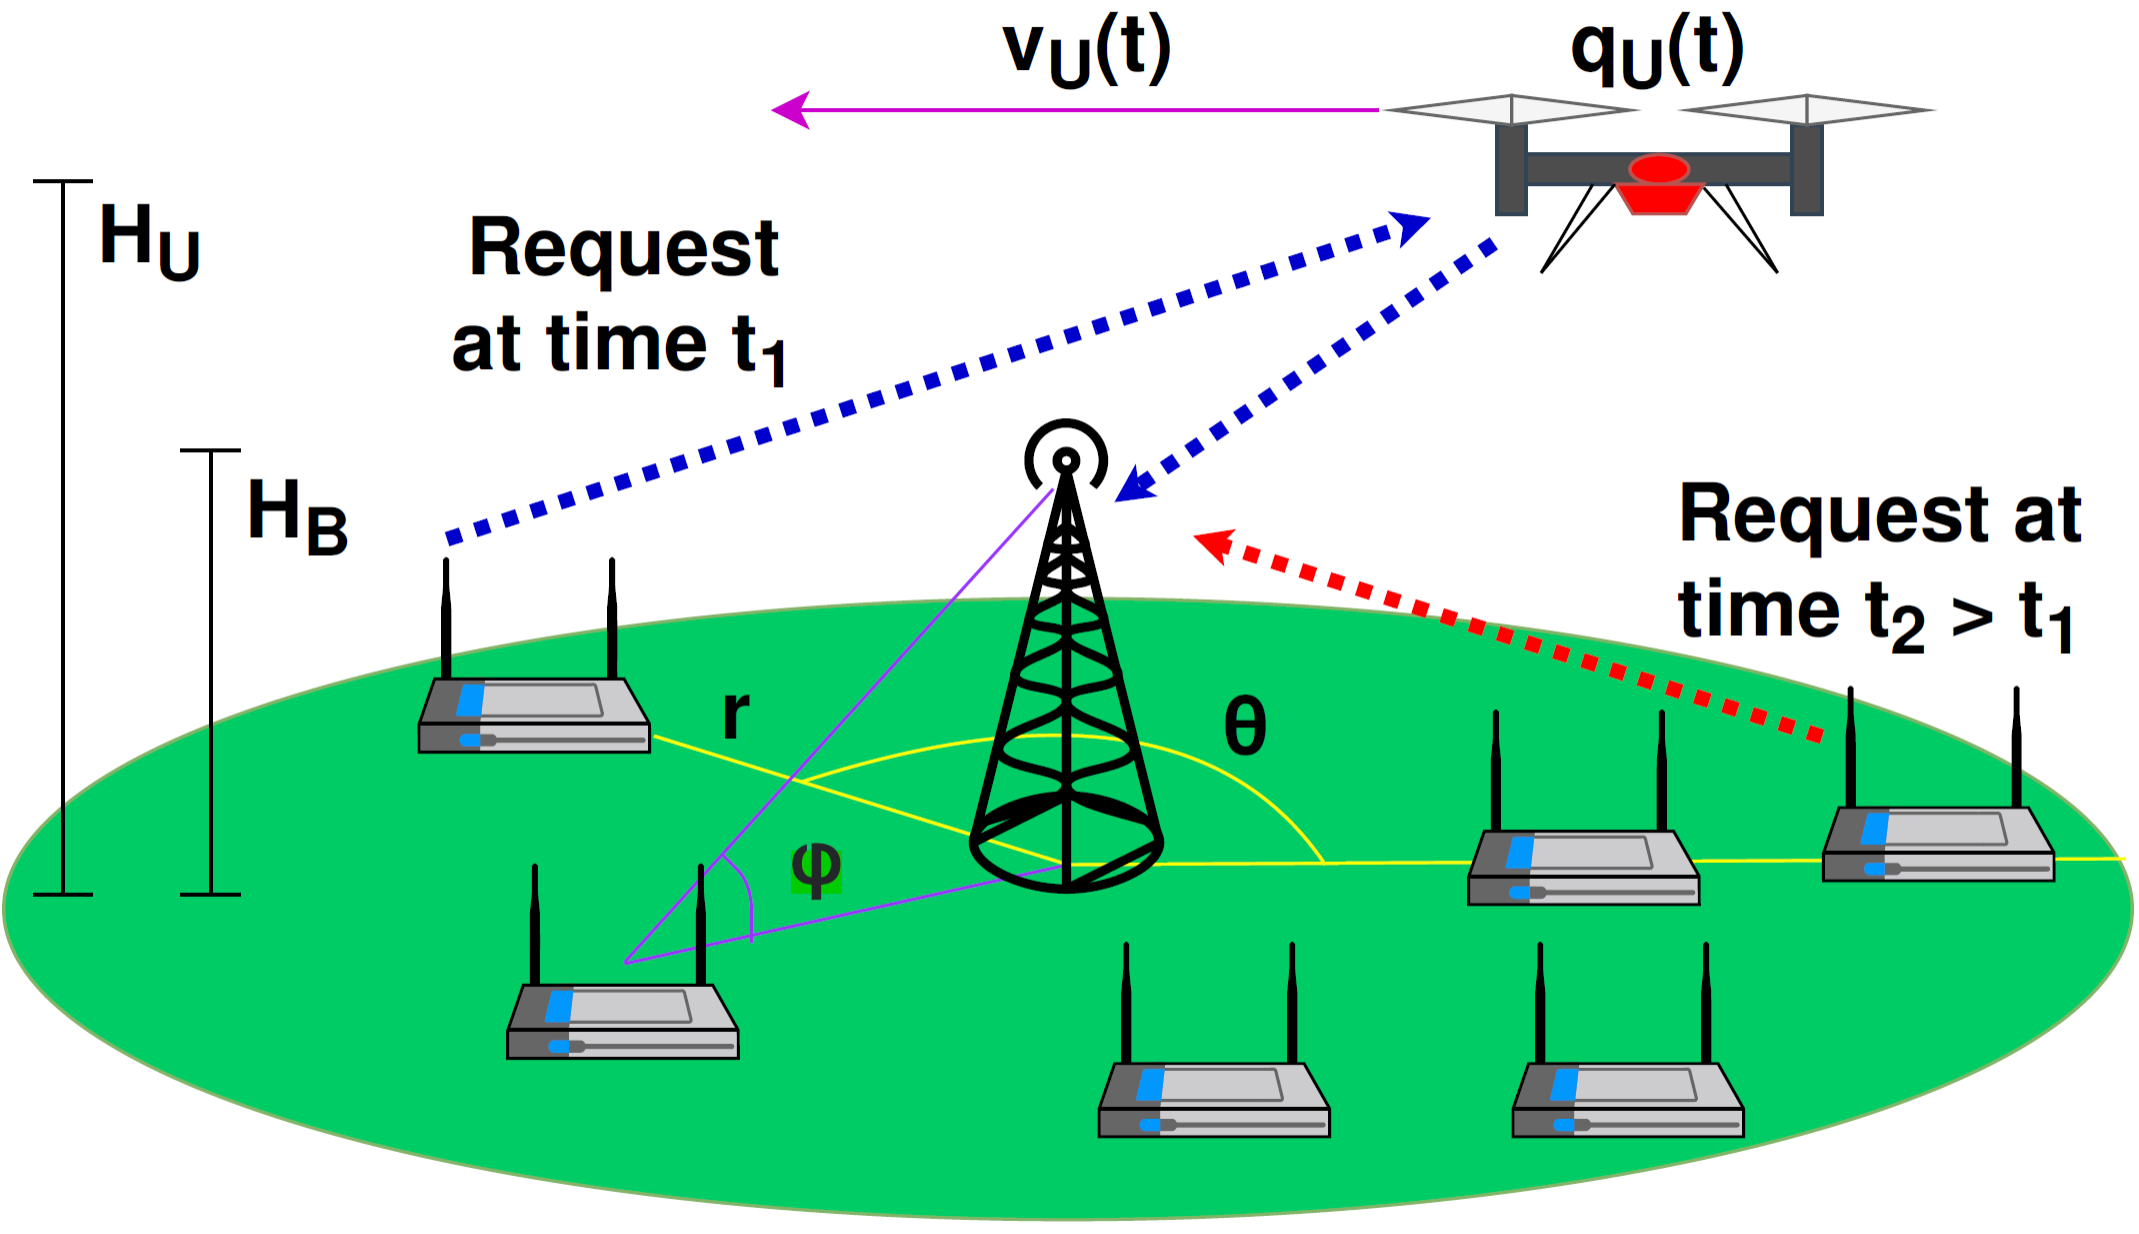
\includegraphics[width=0.7\linewidth]{figs/System_Architecture_II.png}
    \caption{A specialization of the generic deployment model discussed in Sec. \ref{S2}: a BS augmented by a single UAV serving as a wireless relay for a random distribution of GNs that are dynamically generating uplink transmission requests according to a Poisson process with rate $\frac{\Lambda}{N_{U}}$ [requests per unit time].}
    \vspace{-8mm}
    \label{F2}
\end{figure}

In this section, studying the setup illustrated in Fig. \ref{F2}, we specialize the deployment model described in Sec. \ref{S2} to the case of a single UAV, and present MAESTRO, a Multiscale Adaptive Energy-conscious Scheduling and TRajectory Optimization framework to minimize the time-average service delay subject to an average UAV mobility power constraint via a Semi-Markov Decision Process (SMDP) formulation. Since we will later extend this model to a swarm of $N_U$ UAVs, each scheduled to serve a portion of the traffic, the traffic rate experienced by a single UAV is $\frac{\Lambda}{N_U}$ [requests per unit time], which is assumed in this section in place of the overall rate $\Lambda$. We let $\mathbf{q}_{U}(t){=}(r_{U}(t),\theta_{U}(t))$ be the polar coordinate of the UAV at time $t$, projected on the $x{-}y$ plane, where $r_{U}(t){\in}\mathbb{R}_{+}$ and $\theta_{U}(t){\in}[0,2\pi)$ denote the UAV's radius and angle with respect to the BS (cell center).

Analyzing this model, we note that the operations of the UAV relay can be split into the following phases. In the \emph{waiting} phase, no GN requests are being served by the UAV, which thus moves according to a waiting policy as described next, until a new request is received. When a new GN request is received, say from position $(r,\theta)$, the system transitions to the \emph{request scheduling} phase, where the system decides if the GN should transmit its data payload directly to the BS, or relay it through the UAV. If direct transmission is selected, the system immediately re-enters the \emph{waiting} phase, as the UAV remains free to serve other requests; else, the system enters the \emph{UAV relay} phase, in which the GN relays its data payload through the UAV using the D\&F protocol described in further detail in this section; upon the completion of this relay service, the system re-enters the \emph{waiting} phase. Here, we simplify our construction by neglecting the waiting times encountered by requests in the BS and UAV queues---specifically, in the \emph{request scheduling} phase, the decision-making scheme takes into account only the communication service times in order to optimally choose between direct-BS and relayed service actions. However, in Sec. \ref{S5}, we supplement our optimal single-relay decision making scheme with studies on M/G/x queueing dynamics (at both the BS and the UAVs) to incorporate queue wait latencies into this scheduling decision. As the BS can accommodate simultaneous transmissions (see Sec. \ref{S2}), new requests received during an \emph{UAV relay} phase (i.e., when the UAV is occupied serving another request) are directly served by the BS.

We define a decision interval as the time duration spanning the start of a \emph{waiting} phase, the subsequent \emph{request scheduling} phase when a GN request is received, until the system re-enters the \emph{waiting} phase after scheduling a direct transmission to the BS, or following the \emph{UAV relay} phase. Consider the $u$th such decision interval; let $\Delta_{u}^{(w)}$ be the time to wait for a new request, and $\Delta_{u}^{(s)}$ be the time to serve it, either through the BS (denoted with the scheduling decision $\xi_{u}{=}0$) or through the UAV ($\xi_{u}{=}1$).  Then, the $u$th decision interval duration is $\Delta_{u}{=}\Delta_{u}^{(w)}{+}\xi_{u}\Delta_{u}^{(s)}$, since the UAV enters the \emph{waiting phase} immediately if a direct transmission to the BS is scheduled.

We now formulate the average communication delay and UAV mobility power. Let $N_{u}{\geq}0$ be the number of additional requests received during the UAV relay phase of the $u$th decision period; since these additional requests are served directly by the BS, let $\Delta_{u,i}^{(bs)},i=\{1,{\dots},N_{u}\}$ be their communication delays. Let $E_{u}$ be the UAV mobility energy expended during the $u$th decision interval. Let $M_{t}$ be the total number of decision intervals completed up to time $t$. Then, we define the expected average communication delay per GN request under a given policy $\mu$ that defines the request scheduling, communication strategy, and UAV trajectory (formally defined later)\footnote{In the following, expectations $\mathbb{E}_{\mu}[\cdot]$ will be implicitly assumed to be conditioned on an arbitrary initial position $\mathbf{q}_{U}(0)$ of the UAV at time $t{=}0$.}, as the total communication delay accrued until time $t$, over the total number of requests served until time $t$; similarly, we define the expected average UAV power as the total energy consumption, over the total duration of the $M_{t}$ decision intervals up to time $t$; mathematically,
\begin{align}\label{eq:DBarMu}
    &\bar{D}_{\mu} \triangleq \lim_{t \rightarrow \infty} \mathbb{E}_{\mu} \Bigg[
    \frac{\frac{1}{M_t}\sum_{u = 1}^{M_t}(\Delta_u^{(s)}+\xi_u\sum_{i=1}^{N_u}\Delta_{u,i}^{(bs)})}{
    \frac{1}{M_t}\sum_{u = 1}^{M_t}(1+\xi_uN_u)
    }\Bigg],\ 	\bar{P}_{\mu} \triangleq \lim_{t \rightarrow \infty} \mathbb{E}_{\mu} \Bigg[ \frac{\frac{1}{M_t}\sum_{u = 1}^{M_t}E_u}{\frac{1}{M_t}\sum_{u = 1}^{M_t} \Delta_u}\Bigg].
\end{align}
Note that $\bar{D}_{\mu}$ in \eqref{eq:DBarMu} captures the delays of all requests, i.e., those relayed through the UAV ($\xi_{u}{=}1$), those transmitted directly to the BS ($\xi_{u}{=}0$), as well as the $N_{u}$ additional requests served directly by the BS during the UAV relay phase.
The goal is to solve\footnote{Without loss of generality, we assume $P_{\mathrm{avg}}\geq\min_{V\geq0}P_{\mathrm{mob}}(V){\triangleq}P_{\min}$, since any $P_{\mathrm{avg}}{<}P_{\min}$ is not feasible.}
\begin{align}\label{eq:OverallObj0}
    &\bar{D}_{\mu}^{*} = \underset{\mu}{\mathrm{min}} \; 
	\bar D_\mu\;\;
	\mathrm{s.t.} \; \bar P_\mu\leq P_{\mathrm{avg}},\text{ with optimal policy $\mu^{*}$.}
\end{align}

To simplify these expressions, let
$\bar{\mathbb{E}}_{\mu}[C_u]\triangleq\lim\limits_{t \rightarrow \infty} \mathbb{E}_{\mu}
[\frac{1}{M_t} \sum_{u = 1}^{M_t }C_u]$ be a shorthand notation to denote the long-term average cost $C_u$ per decision interval, and let
\begin{align}\label{eq:BarDefs}
    \bar{E}_{\mu}{\triangleq}\bar{\mathbb{E}}_{\mu} \left[E_u\right],
    \bar{T}_{\mu}{\triangleq}\bar{\mathbb{E}}_{\mu} \left[\Delta_u\right],
    \bar{N}_{\mu}{\triangleq}\bar{\mathbb{E}}_{\mu} \left[1+\xi_uN_u\right],
    \bar{W}_{\mu}^{(s)}{\triangleq}\bar{\mathbb{E}}_{\mu}\left[\Delta_u^{(s)}\right],
    \bar{W}_{\mu}^{(bs)}{\triangleq}\bar{\mathbb{E}}_{\mu}\left[\xi_u\sum_{i=1}^{N_u}\Delta_{u,i}^{(bs)}\right]
\end{align}
be the expected average UAV energy expenditure ($\bar{E}_{\mu}$), duration ($\bar{T}_{\mu}$), number of requests served ($\bar{N}_{\mu}$), delay of requests for which a scheduling decision is made ($\bar{W}_{\mu}^{(s)}$), and total delays of requests served directly by the BS during the UAV relay phase
($\bar{W}_{\mu}^{(bs)}$), per decision interval, under policy $\mu$. We can then write $\bar{P}_{\mu}{=}\frac{\bar{E}_{\mu}}{\bar{T}_{\mu}}$ and $\bar{D}_{\mu}{=}\frac{\bar{W}_{\mu}^{(s)}+\bar{W}_{\mu}^{(bs)}}{\bar{N}_{\mu}}$ (Little's Law \cite{LittlesLaw}), yielding the equivalent optimization problem
\begin{align}\label{eq:OverallObj1}
    &\bar{D}_{\mu}^{*} = \underset{\mu}{\mathrm{min}} \; 
	\frac{\bar{W}_{\mu}^{(s)}+\bar{W}_{\mu}^{(bs)}}{\bar{N}_{\mu}}\;\;
	\mathrm{s.t.} \; \bar{E}_{\mu}-P_{\mathrm{avg}}\bar{T}_{\mu}\leq 0.
\end{align}

Under the optimal policy, $\bar{D}_{\mu}^{*}{\leq}\bar{D}_{BS}$ (in fact, a feasible policy is obtained by serving all requests directly by the BS while the UAV flies at the power minimizing velocity). This suggests that optimization of the UAV trajectory and scheduling decisions is key to improving the delay performance to serve requests. Note the inherent complexity that is required to solve the optimization problem \eqref{eq:OverallObj1}: as the policy varies, the delay metric changes both the numerator and denominator terms of the objective function, which cannot be solved with standard dynamic programming algorithms. To address this challenge, we now propose an alternative optimization criterion based on upper- and lower-bounds to $\bar{D}_{\mu}$ (Lemma \ref{lem:UpLowB}, whose proof is provided in Appendix A).

\begin{lemma}\label{lem:UpLowB}
Under any policy $\mu$ such that $\bar{W}_{\mu}^{(s)}{\leq}\bar{D}_{BS}$ (including the optimal $\mu^{*}$), we have that
\begin{align}\label{eq:ULBound}
    &\bar{W}_{\mu}^{(s)}\leq\bar{D}_{\mu}
    \leq \bar{W}_{\mu}^{(s)}\frac{1+\Lambda\bar{D}_{BS}}{1+\Lambda\bar{W}_{\mu}^{(s)}}
    \leq \bar{D}_{BS}.
\end{align}
\end{lemma}

Remarkably, the lower and upper bounds of $\bar{D}_{\mu}$ are both increasing functions of $\bar{W}_{\mu}^{(s)}$; hence, we will use $\bar{W}_{\mu}^{(s)}$ as a surrogate to minimize the expected delay $\bar D_\mu$. This observation motivates us to look at the alternative optimization problem
\begin{align}\label{eq:StdW2}
    &\underset{\mu}{\mathrm{min}} \; 
    \bar{W}_{\mu}^{(s)}
    \ 	\mathrm{s.t.} \; \bar{E}_{\mu}-P_{\mathrm{avg}}\bar{T}_{\mu}\leq 0,
\end{align}
which will be the focus of the following analysis. To solve it, we use the Lagrangian formulation
\begin{align}\label{eq:W2Lagr}
    &g(\nu){=}\underset{\mu}{\mathrm{min}} \left( \bar{W}_{\mu}^{(s)} + \nu (\bar{E}_{\mu}-P_{\mathrm{avg}}\bar{T}_{\mu}) \right)
    {=}\underset{\mu}{\mathrm{min}}\, \bar{\mathbb E}_\mu\left[\Delta_u^{(s)} + \nu (E_u - P_{\mathrm{avg}}\Delta_u)\right],\!\!
\end{align}
where $\nu$ is the dual variable, optimized by solving $\max_{\nu{\geq}0}g(\nu)$. We now demonstrate that for a given $\nu{\geq}0$, \eqref{eq:W2Lagr} can be cast as a Semi-Markov decision process (SMDP) and solved with dynamic programming tools. We first characterize the states, actions, and policy of this SMDP. 

\noindent{\textbf{States}}: The state is defined by the UAV position $\mathbf{q}_{U}$, taking value from the set $\mathcal{Q}_{\mathrm{UAV}}\triangleq\mathbb{R}_{+}\times[0,2\pi)$ (in polar coordinates), and the position of an uplink transmission request $\mathbf{q}_G$, taking values from $\mathcal{Q}_{\mathrm{GN}}{\triangleq}[0,a]{\times}[0,2\pi)$ (polar coordinates). The state space is then $\mathcal{S}{=}\mathcal{S}_{\mathrm{wait}}{\cup}$ $\mathcal{S}_{\mathrm{comm}}$, where $\mathcal{S}_{\mathrm{wait}}{=}\mathcal{Q}_{\mathrm{UAV}}$ is the set of \emph{waiting} states and $\mathcal{S}_{\mathrm{comm}}{=}\mathcal{Q}_{\mathrm{UAV}}{\times}\mathcal{Q}_{\mathrm{GN}}$ is the set of \emph{communication} states. Crucial to the definition of the SMDP is how the system is sampled in time to define Markov dynamics in the evolution of the sampled states, as specified below. Accordingly, we define the actions available in each state $\mathbf{s}{\in}\mathcal{S}$ and the transition probabilities, along with the duration $T(\mathbf{s};\mathbf{a})$, the UAV energy usage $E(\mathbf{s};\mathbf{a})$, and the communication delay $\Delta(\mathbf{s};\mathbf{a})$ metrics accrued in state $\mathbf{s}$ under action $\mathbf{a}$.

\noindent{\textbf{Waiting states' actions, transitions, and metrics}}: If the UAV is in the \emph{waiting} state $\mathbf{s}_{n} = \mathbf{q}_{U} \in \mathcal{S}_{\mathrm{wait}}$ at time $t$, i.e., it is in position $\mathbf{q}_{U}(t){=}\mathbf{q}_{U}{=}(r_{U},\theta_{U})$ with no active requests, then the actions available are to move the UAV with radial (referred to the outward direction) and angular (referred counter-clockwise) velocity components $(v_{r},\theta_{c})$, over an arbitrarily small duration $\Delta_{0}{\ll}1/\Lambda$. Under a maximum velocity constraint $V_{\mathrm{max}}$, the action space is then 
\begin{align}\label{eq:WaitActions}
	\mathcal{A}_{\mathrm{wait}}(r_U) \triangleq \Big\{(v_{r},\theta_{c}) \in \mathbb R^{2} \, \Big| \, \sqrt{v_{r}^{2} + r_U^2\cdot \theta_{c}^{2}}\leq V_{\mathrm{max}} \Big\},
\end{align}
where $v_{U}=\sqrt{v_{r}^{2}{+}r_{U}^{2}\theta_{c}^{2}}$ is the velocity expressed with respect to polar coordinates. Upon choosing action $\mathbf{a}{=}(v_{r},\theta_{c}){\in}\mathcal{A}_{\mathrm{wait}}(r_{U})$, the communication delay is $\Delta(\mathbf{s};\mathbf{a}){=}0$, since there is no ongoing communication; the duration of a waiting state visit is $T(\mathbf{s};\mathbf{a}){=}\Delta_{0}$, during which the UAV uses an amount of energy $E(\mathbf{s};\mathbf{a}){=}\Delta_{0}P_{\mathrm{mob}} \left(v_{U}\right)$ to move at velocity $v_{U}$.

The new state is then sampled at time $t{+}\Delta_{0}$, with the UAV moved to the new position $\mathbf{q}_{U}(t{+}\Delta_{0}){\approx}(r_{U},\theta_{U}){+}(v_{r},\theta_{c})\Delta_{0}$. With probability $e^{-\Lambda \Delta_{0}}$, no new request is received in the time interval $[t,t{+}\Delta_{0}]$, so that the new state is a waiting state.  Otherwise, a new request is received from a GN in position $(r,\theta)$, so that the new state is a communication state. Thus, the transition probability from the waiting state $\mathbf{s}_{n}{=}(\mathbf{q}_{U},\mathbf{w}_{0})$ under action $\mathbf{a}_{n}{=}(v_{r},\theta_{c}){\in}\mathcal{A}_{\mathrm{wait}}(r_{U})$ is 
\begin{align}\label{eq:CommTransProb}
    &\mathbb{P}(\mathbf{s}_{n+1}=\mathbf q_U+\mathbf a_n\Delta_0|\mathbf{s}_n,\mathbf{a}_n) = e^{-\Lambda \Delta_{0}},\\\label{eq:R0ContTrProb}
    &\mathbb{P}(\mathbf{s}_{n+1}=(\mathbf q_U+\mathbf a_n\Delta_0,\mathbf q_G') \text{ with } \mathbf q_G' \in \mathcal{F} \,|\mathbf{s}_n,\mathbf{a}_n) =\frac{A(\mathcal{F})}{\pi a^2} \cdot (1-e^{-\Lambda \Delta_{0}}),\ \forall \mathcal{F}\subseteq \mathcal{Q}_{\mathrm{GN}},
\end{align}
where $A(\mathcal{F})$ is the area of region $\mathcal{F}$, since requests are uniformly distributed in the cell.

\noindent{\textbf{Communication states' actions, transitions, and metrics}}:
Upon reaching a communication state $\mathbf{s}_{n}{=}(\mathbf{q}_{U},\mathbf{q}_{G}){\in}\mathcal{S}_{\mathrm{comm}}$ at time $t$, the system must serve a GN request at position $\mathbf{q}_{G}=(r,\theta)$. The BS first determines the scheduling decision $\xi{\in}\{0,1\}$. If $\xi{=}0$, the GN transmits directly to the BS, and the next state is sampled immediately after the decision, so that it is the waiting state $\mathbf{s}_{n{+}1}{=}\mathbf{q}_{U}{\in}\mathcal{S}_{\mathrm{wait}}$ with probability $1$. In this case, the cost metrics under action $\mathbf{a}_{n}{=}\mathbf{a}{=}(0,[\ ])$ are computed as $\Delta(\mathbf{s}_{n};\mathbf{a}){=}\frac{L}{\bar R_{GB}(r)}$, $E(\mathbf{s}_{n};\mathbf{a}){=}0$, $T(\mathbf{s}_{n};\mathbf{a}){=}0$, since direct transmissions occur at throughput $\bar{R}_{GB}(r)$ and the system moves immediately to the waiting state $\mathbf{q}_{U}{\in}\mathcal{S}_{\mathrm{wait}}$ resulting in the action duration and energy expenditure being $0$. 

On the other hand, if $\xi{=}1$, the UAV uses the D\&F protocol described next, while following a trajectory starting from its current position $\mathbf{q}_{U}$ and ending in position $\mathbf{q}_{U}'$. We denote this action as $\mathbf{a}_{n}{=}\mathbf{\tilde{a}}{=}(1,\mathbf{q}_{U}{\rightarrow}{\mathbf{q}}_{U}')$. In the first phase (of duration $t_{p}$) of the D\&F protocol, the GN transmits its payload to the UAV; in the second phase (of duration $\Delta{-}t_{p}$), the UAV relays the data payload to the BS. Assuming a \emph{move-and-transmit} implementation \cite{SCA}, the trajectory ($\mathbf{q}_{U}{\rightarrow}{\mathbf{q}}_{U}'$) and the durations ($t_{p}$ and $\Delta{-}t_{p}$) must satisfy
\begin{align}\label{eq:PLConst0}
	\int_{0}^{t_{p}} \bar{R}_{GU}(r_{GU}(t+\eta)) \mathrm d \eta \geq L, \ \int_{t_p}^{\Delta} \bar R_{UB}(r_{UB}(t+\eta)) \mathrm d \eta \geq L,
\end{align}
i.e., the entire payload of $L$ bits is first transmitted to the UAV with rate $\bar R_{GU}(r_{GU}(t{+}\eta))$, where $r_{GU}(t{+}{\eta})$ is the GN-UAV distance (projected onto the $x{-}y$ plane) at time $t{+}\eta$; then, the UAV transmits the payload to the BS with rate $\bar{R}_{UB}(r_{UB}(t{+}\eta))$, where $r_{UB}(t{+}\eta)$ is the radial position of the UAV at time $t{+}\eta$, so that the total communication delay is $\Delta$.  In this case, the cost metrics under action $\mathbf{\tilde{a}}$ are $\Delta(\mathbf{s}_{n};\mathbf{\tilde{a}}){=}\Delta$, $E(\mathbf{s}_{n};\mathbf{\tilde{a}}){=}\int_0^\Delta P_{\mathrm{mob}}\left(v_{U}(t{+}\eta)\right)\mathrm{d}\eta$, $T(\mathbf{s}_{n};\mathbf{\tilde{a}}){=}\Delta$. Upon completing the D\&F protocol, the UAV enters the \emph{waiting} phase again, so that $\mathbf{s}_{n{+}1}{=}\mathbf{q}_{U}'$ becomes the new SMDP state, sampled at time $t{+}\Delta$. Let $\mathcal{Q}_{\mathbf{q}_{G}}\big(\mathbf{q}_{U}{\rightarrow}{\mathbf{q}}_{U}'\big)$ be the set of feasible UAV trajectories starting in $\mathbf{q}_{U}$, terminating in $\mathbf{q}_{U}'$, to serve a GN located at $\mathbf{q}_{G}$ via the D\&F protocol, i.e.,
\begin{align}
	\mathcal{Q}_{\mathbf q_G} \big({\mathbf q}_U\rightarrow{\mathbf q}_U'\big) = \Big\{ &\mathbf{p}_{U} : 
	[0,\Delta] \mapsto \mathbb{R}_{+} \times[0,2\pi)\text{ s.t.}\\
	&\int_{0}^{t_{p}} \bar{R}_{GU}(r_{GU}(t+\eta)) \mathrm d \eta \geq L, \ \int_{t_p}^{\Delta} \bar R_{UB}(r_{UB}(t+\eta)) \mathrm d \eta \geq L, \label{eq:PLConst1}\tag{C.1}\\
	&v_U (\eta) \leq V_{\mathrm{max}},\ \forall\eta\in[0,\Delta],\label{eq:SpeedConst1}\tag{C.2}\\
	&\mathbf{p}_{U}(0) ={\mathbf q}_U, 
	\mathbf{p}_{U}(\Delta) ={\mathbf q}_U',\label{eq:IFConst1}\ \exists \Delta \geq 0, \exists\; 0 \leq t_p \leq \Delta 
	\Big\},
	\tag{C.3}
\end{align}
where \ref{eq:PLConst1} reflects the data payload constraints, \ref{eq:SpeedConst1} the maximum velocity constraint, and \ref{eq:IFConst1} the trajectory constraints. Then, the action space in state $(\mathbf{q}_{U},\mathbf{q}_{G}){\in}\mathcal{S}_{\mathrm{comm}}$ when $\xi{=}1$ is the set $\mathcal{Q}_{\mathbf{q}_{G}}(\mathbf{q}_{U}){\triangleq}\cup_{\mathbf{q}_{U}'{\in}\mathcal{Q}_{\mathrm{UAV}}}\mathcal{Q}_{\mathbf{q}_{G}}\big(\mathbf{q}_{U}{\rightarrow}\mathbf{q}_{U}'\big)$ of feasible trajectories starting in $\mathbf{q}_{U}$ that serve the GN at $\mathbf{q}_{G}$ via the D\&F protocol. The overall action space of the \emph{communication} states $(\mathbf{q}_{U},\mathbf{q}_{G}){\in}\mathcal{S}_{\mathrm{comm}}$ is then $\mathcal{A}_{\mathrm{comm}}(\mathbf{q}_{U},\mathbf{q}_{G}){\triangleq}\{0,[\ ]\}{\cup}\{\{1\}{\times}\mathcal{Q}_{r,\theta}(r_{U},\theta_{U})\}$. Here the set $\{0, [\ ]\}$ is associated with the decision $\xi{=}0$ (direct-BS) and hence, there is no trajectory design space corresponding to it; while the set $\{\{1\}{\times}\mathcal{Q}_{r,\theta}(r_{U},\theta_{U})\}$ is associated with the decision $\xi{=}1$ (relayed service) whose trajectory design space is $\mathcal{Q}_{r,\theta}(r_{U},\theta_{U})$.

\noindent{\textbf{Policy $\mu$}}: For \emph{waiting} states $\mathbf{q}_{U}{\in}\mathcal{S}_{\mathrm{wait}}$, the policy selects a velocity $(v_{r},\theta_{c})$ from the action space defined in \eqref{eq:WaitActions}, i.e., $\mu(\mathbf{q}_{U}){\in}\mathcal{A}_{\mathrm{wait}}(r_{U})$. Likewise, for \emph{communication} states $(\mathbf{q}_{U},\mathbf{q}_{G}){\in}\mathcal{S}_{\mathrm{comm}}$, the policy selects the scheduling decision $\xi{\in}\{0,1\}$ and, if $\xi{=}1$, the trajectory followed in the D\&F protocol, i.e., $\mu(\mathbf{q}_{U},\mathbf{q}_{G}){\in}\mathcal{A}_{\mathrm{comm}}(\mathbf{q}_{U},\mathbf{q}_{G})$.

With a stationary policy $\mu$ defined, the Lagrangian metric $L_{\mu}^{(\nu)}{\triangleq}\bar{W}_{\mu}^{(s)}{+}\nu(\bar{E}_{\mu}{-}P_{\mathrm{avg}}\bar{T}_{\mu})$ in \eqref{eq:W2Lagr} is reformulated using Little's Law \cite{LittlesLaw} in terms of the SMDP steady-state probabilities as
\begin{align}\label{eq:CostMetric}
    L_\mu^{(\nu)}
    = \lim_{N \rightarrow \infty} \mathbb{E}_\mu \Bigg[ \frac{\frac{1}{N}\sum_{n=0}^{N-1}  \ell_\nu(\mathbf{s}_n; \mu(\mathbf{s}_n)) }{\frac{1}{N}\sum_{n = 0}^{N-1} \mathbb I(\mathbf{s}_n \in \mathcal{S}_{\mathrm{comm}})}  \Bigg]
    = \frac{1}{\pi_{\mathrm{comm}}}\int_{\mathcal{S}} \Pi_{\mu}(\mathbf{s})\ell_\nu(\mathbf{s}; \mu(\mathbf{s}))\mathrm{d}\mathbf{s},
\end{align}
where $\Pi_{\mu}(\mathbf{s})$ is the steady-state probability density function of the SMDP being in a state $\mathbf{s}$ under policy $\mu$, $\pi_{\mathrm{comm}}{=}\int_{\mathcal{S}_{\mathrm{comm}}}\!\!\!\!\!\Pi_{\mu}(\mathbf{s})\mathrm{d}\mathbf{s}$ is the steady-state probability that the UAV is in the communication phase in the SMDP, whose expression is provided in Appendix B, and $\ell_{\nu}(\mathbf{s};\mathbf{a}) \triangleq \Delta(\mathbf{s};\mathbf{a}){+}\nu\big(E(\mathbf{s};\mathbf{a}){-}P_{\mathrm{avg}}T(\mathbf{s};\mathbf{a})\big)$ is the overall Lagrangian metric in state $\mathbf{s}$ under action $\mathbf{a}$. In \eqref{eq:CostMetric}, note that $\sum_{n=0}^{N{-}1}\ell_{\nu}(\mathbf{s}_{n};\mu(\mathbf{s}_{n}))$ is the total Lagrangian cost accrued during the first $N$ SMDP stages, and $\sum_{n{=}0}^{N{-}1}\mathbb{I}(\mathbf{s}_{n}{\in}\mathcal{S}_{\mathrm{comm}})$ is the number of communication states encountered in the SMDP; since a new decision interval is initiated after a communication state, this in turn equals the number of decision intervals. Therefore, after taking the expectation and the limit $N{\to}\infty$, $L_{\mu}^{(\nu)}$ represents the expected Lagrangian cost per decision interval, as expressed in \eqref{eq:W2Lagr}. The right hand expression in \eqref{eq:CostMetric} follows by noticing that the SMDP achieves a steady-state behavior when $N\to\infty$.

We now specialize the Lagrangian metric $\ell_{\nu}(s;\mathbf{a})$. Specifically, for waiting states,
\begin{align}\label{eq:EllWait}
    \ell_\nu(r_U,\theta_U; v_r,\theta_c)
    =\nu \Big(P_{\mathrm{mob}} \Big(\sqrt{v_{r}^{2} + r_U^2\theta_{c}^{2}}\Big)- P_{\mathrm{avg}} \Big)\Delta_0;
    \end{align}
    for \emph{communication} states under action $\xi=0$, $\ell_{\nu}(r_U,\theta_U,r,\theta; 0, [\ ]) = \frac{L}{\bar{R}_{GB}(r)}$; and for \emph{communication} states under action $\xi=1$ with trajectory 
    $\mathbf p_U$ of duration $\Delta$, we obtain
    \begin{align}\label{eq:EllComm}
    \ell_\nu(r_U,\theta_U,r,\theta; 1,\mathbf p_U)
    \triangleq(1-\nu P_{\mathrm{avg}})\Delta + \nu \int_0^\Delta P_{\mathrm{mob}} \left(v_U (\eta) \right)\mathrm d\eta.
\end{align}
The minimization problem of \eqref{eq:W2Lagr} can then be expressed as the \emph{average cost-per-stage problem}
\begin{align}\label{eq:TotalGMin}
	g(\nu) = \frac{1}{\pi_{\mathrm{comm}}}\underset{\mu}{\mathrm{min}} \; \int_{\mathcal{S}} \Pi_{\mu}(s) 
	\ell_\nu(s; \mu(s))\mathrm d s,
\end{align}
solvable through standard dynamic programming approaches, after discretization of the state space, followed by the dual maximization $\mathrm{max}_{\nu{\geq}0}g(\nu)$.

Since GN transmission requests are uniformly distributed in the circular cell with the BS in the center, the UAV radius information is a sufficient statistic in decision making for a \emph{waiting} state $(r_{U},\theta_{U})$, which can be thus expressed as $\mathbf{s}{=}r_{U}{\in}\mathcal{S}_{\mathrm{wait}}$. Likewise, for a \emph{communication} state $(r_{U},\theta_{U},r,\theta)$, only the UAV radius, GN request radius, and the angle $\psi{\in}[0,2\pi)$ between them suffice to characterize the state. Thus \emph{communication} states can be compactly represented as $\mathbf{s}{=}(r_{U},r,\psi){\in}\mathcal{S}_{\mathrm{comm}}$. A consequence of these sufficient statistics for decision making is that the policy affects the SMDP state transitions (hence steady-state behavior) only through the UAV radial velocity $v_{r}$ in the \emph{waiting} states and the UAV trajectory's target end radius position $\hat{r}_{U}$ in the \emph{communication} states. On the other hand, the angular velocity $\theta_{c}$ in the \emph{waiting} states and the UAV trajectory's target end angular coordinate $\hat{\theta}_{U}$ in the \emph{communication} states do not influence state dynamics, but only the instantaneous Lagrangian metric $\ell_{\nu}$.

With this observation, let $O(\mathbf{s}){\triangleq}v_{r}{\in}[-V_{\mathrm{max}},V_{\mathrm{max}}]$ define the radial velocity policy of the \emph{waiting} states $\mathbf{s}{\in}\mathcal{S}_{\mathrm{wait}}$, specifying the radial velocity component of a waiting action $\mathbf{a}{=}(v_{r},\theta_{c}) \in \mathcal{A}_{\mathrm{wait}}(\mathbf{s})$; let $U(\mathbf{s}){\triangleq}\hat{r}_{U}{\in}[0,a]$ define the next radius position policy of the \emph{communication} states $\mathbf{s}{\in}\mathcal{S}_{\mathrm{comm}}$, specifying the end radius position of a scheduling and communication action $\mathbf{a}{\in}\mathcal{A}_{\mathrm{comm}}(\mathbf{s})$. Under this decomposition, $O$ and $U$ constitute the outer decisions made by the SMDP and are the only actions to affect the steady-state distribution, denoted as $\Pi_{O,U}$ under the outer policy $(O,U)$. Thus, the optimization problem \eqref{eq:TotalGMin} can be restated as
\begin{align}\label{eq:PolDecomp}
	g(\nu) = \frac{1}{\pi_{\mathrm{comm}}} \underset{O,U}{\mathrm{min}} \Bigr[ \int_{\mathcal{S}_{\mathrm{wait}}} \Pi_{O,U}(\mathbf{s}) \ell_{\nu}^{*}(\mathbf{s}; O(\mathbf{s}))\mathrm{d}\mathbf{s} + \int_{\mathcal{S}_{\mathrm{comm}}} \Pi_{O,U}(\mathbf{s}) \ell_{\nu}^{*}(\mathbf{s}; U(\mathbf{s})) \mathrm{d}\mathbf{s} \Bigr],
\end{align}
where $\ell_{\nu}^{*}$ is the Lagrangian metric optimized with respect to the \emph{inner action} components not specified by $O$ and $U$. In particular, for waiting states $\mathbf{s}{=}r_{U}$ and radial velocity $O(\mathbf{s}){=}v_{r}$, the inner optimization is performed with respect to the UAV angular velocity $\theta_{c}$, i.e.,
\begin{align}\label{eq:MinLWP}
	&\ell_{\nu}^{*}(\mathbf{s}; v_r) = \underset{\theta_c}{\mathrm{min}}\; \nu \left( P_{\mathrm{mob}}\left(\sqrt{v_{r}^2 + r_U^2\theta_c^2}\right) - P_{\mathrm{avg}} \right)\Delta_0 \;\; \mathrm{s.t.}\;\; \sqrt{v_{r}^{2} + r_U^2\theta_c^2} \leq V_{\mathrm{max}}.
\end{align}
Since $\nu{\geq}0$, $\Delta_{0}{>}0$, and $P_{\mathrm{avg}}$ are constant, the optimizer $\theta_{c}^{*}$ is the angular velocity minimizing the UAV power consumption for a given UAV radial velocity $v_{r}$ and radius $r_{U}$, solvable through exhaustive search. For communication states $\mathbf{s}{=}(r_{U},r,\psi)$, $\ell_{\nu}^{*}(\mathbf{s};\hat{r}_{U})$ is determined by optimizing over the scheduling decision $\xi{\in}\{0,1\}$ and, if $\xi{=}1$, the trajectory $\mathbf{p}_{U}$ followed by the UAV, terminating at the radial position $\hat{r}_{U}$. To formalize it, let $\ell_{\nu}^{*}(\mathbf{s};\hat{r}_{U},\xi)$ denote the optimized metric as a function of $\xi{\in}\{0,1\}$. For $\xi{=}1$ (D\&F protocol),
\begin{align}
    &\ell_{\nu}^{*}(\mathbf{s};\hat r_U,1) = \underset{\Delta,\mathbf{p}_U,t_p}{\mathrm{min}}\; (1-\nu P_{\mathrm{avg}}) \Delta + \nu \int_{0}^{\Delta} P_{\mathrm{mob}}\Bigg( \sqrt{r_U^{'}(\eta)^{2} + r_{U}^{2}(\eta)\theta_{U}^{'}(\eta)^{2}} \Bigg)\mathrm{d} \eta \label{eq:EllMin}\\
    &\mathrm{s.t.}\;\, \text{\ref{eq:PLConst1}},\; \text{\ref{eq:SpeedConst1}},\nonumber\\
    &\mathbf{p}_{U}(0) =(r_U,0), \Vert \mathbf{p}_{U}(\Delta)\Vert_{2} =\hat{r}_U,\tag{$\hat{\text{C}}$.3}\label{eq:StEnd}\
\end{align}
where \ref{eq:PLConst1} reflects the data payload constraints of the D\&F protocol, \ref{eq:SpeedConst1} is the maximum UAV velocity constraint, and \ref{eq:StEnd} (rewritten version of \ref{eq:IFConst1}) enforces the trajectory constraints. For $\xi{=}0$ (direct-BS, hence $\hat{r}_{U}{=}r_{U}$\footnote{Note that with direct transmission to the BS, the system immediately transitions to the waiting state $r_{U}$ with the UAV at distance $r_{U}$ from the center, hence $\hat{r}_{U}{=}r_{U}$ in this case.}), $\ell_{\nu}^{*}(\mathbf{s};r_{U},0){=}\frac{L}{\bar{R}_{GB}(r)}$, hence $\ell_{\nu}^{*}(\mathbf{s};r_{U})$ is obtained by further minimizing over the scheduling decision $\xi{\in}\{0,1\}$, yielding
\begin{align}\label{ellnushatru}
	\ell_{\nu}^* (\mathbf{s}; \hat r_U) = \underset{\xi\in\{0,1\}}{\min} \ell_{\nu}^* (\mathbf{s}; r_U,\xi)\mathbb{I}(\hat r_U = r_U) + \ell_{\nu}^* (\mathbf{s}; \hat r_U, 1)\mathbb{I} (\hat r_U \neq r_U).
\end{align}
Thus, if the outer decision selects $U(\mathbf{s}){=}r_{U}$, the inner scheduling decision $\xi{\in}\{0,1\}$ is obtained by greedily minimizing 
a cost metric that trades off communication delay and energy consumption, i.e., direct transmission to the BS occurs if $\ell_{\nu}^{*}(\mathbf{s}; r_{U},0){<}\ell_{\nu}^{*}(\mathbf{s};r_{U},1)$. Otherwise, the UAV handles the GN request using the D\&F protocol, and the inner decision on UAV trajectory greedily minimizes the instantaneous delay-power trade-off, terminating at the target radius of the outer decision, $U(\mathbf{s}){=}\hat{r}_{U}$.

The optimization problem \eqref{eq:EllMin} will be the focus of Sec. \ref{S4}. We now describe Algorithm \ref{A1}, which designs the outer policy and computes the average cost-per-stage metric $g(\nu)$, along with the average energy- and time-per-stage metrics for a given $\nu$, by solving problem \eqref{eq:PolDecomp} via value iteration. Here, we also discuss Algorithm \ref{A2}, which solves the dual maximization problem $\mathrm{max}_{\nu{\geq}0},g(\nu)$ via projected sub-gradient ascent \cite{SubgradientMethods}.

Specifically\footnote{Although the pseudo-code in Algorithm \ref{A1} is defined on continuous state and action spaces, in a practical implementation, these spaces are discretized, so the integrals would be replaced by sums.}, in Algorithm \ref{A1}, lines $2$ and $3$ compute the inner Lagrangian cost metric optimized with respect to the inner actions---along with the energy and time cost metrics---for all states and outer actions; line $6$ computes the value iteration update for waiting states, which accounts for the transition to the waiting state $r_{U}{+}v_{r}\Delta_{0}$ (if no transmission request is received, w.p. $e^{-\Lambda\Delta_{0}}$) and to a communication state $(r_{U}{+}v_{r}\Delta_{0},r',\psi')$ (if a transmission request is received in position $(r',\psi')$, with probability density function $\frac{1}{2\pi}\frac{2r'}{a^{2}}$); line $11$ computes the value iteration update for communication states which---for end radius $\hat{r}_{U}$---accounts for the transition to the waiting state $\hat{r}_{U}$, w.p. $1$; lines $7$, $8$, $12$, and $13$ update the corresponding total energy and time costs; line $17$ estimates the values of the average cost-, energy-, and time-per-stage metrics.

\begin{algorithm}[t]
\caption{Value Iteration: $(O^{*},U^{*},g(\nu),\bar{E},\bar{T})=\mathrm{VITER}(\nu)$}\label{A1}
    \begin{algorithmic}[1]
        \State \textbf{Initialization}: $i{=}0$; the value function $V_{i}(\mathbf{s}){=}0$, total energy cost $E_{i}(\mathbf{s}){=}0$, and total time cost $T_{i}(\mathbf{s}){=}0$, for all states $\mathbf{s}{\in}\mathcal{S}$; stopping criterion $\delta$.
        \vspace{.2cm}
    	\State \textbf{Inner optimization in waiting states}: ${\forall}\mathbf{s}{\in}\mathcal{S}_{\mathrm{wait}}, {\forall}v_{r}{\in}[-V_{\mathrm{max}},V_{\mathrm{max}}]$, calculate $\ell_{\nu}^{*}(\mathbf{s};v_{r})$ as in \eqref{eq:MinLWP}, with minimizer $\theta_{c}^{*}$; compute energy cost $e^{*}(\mathbf{s};v_{r}){=}E(\mathbf{s};v_{r},\theta_{c}^*)$ and time cost $t^{*}(\mathbf{s};v_r){=}T(\mathbf{s};v_{r},\theta_{c}^{*})$.
    	\vspace{.2cm}
    	\State \textbf{Inner optimization in communication states}: ${\forall}\mathbf{s}{\in}\mathcal{S}_{\mathrm{comm}}, {\forall}\hat{r}_{U}{\in}[0,a]$, calculate $\ell_{\nu}^{*}(\mathbf{s};\hat{r}_{U})$ as in \eqref{eq:EllMin} and \eqref{ellnushatru}, with minimizer $(\xi^{*},\hat{\theta}_{U}^{*},\mathbf{p}_{U}^{*},\Delta^{*})$; compute energy cost $e^{*}(\mathbf{s};\hat{r}_{U}){=}\xi^{*}E(\mathbf{s};\hat{r}_{U},\hat{\theta}_{U}^{*},\mathbf{p}_{U}^{*})$ and time cost $t^{*}(\mathbf{s};\hat{r}_{U}){=}\xi^{*}T(\mathbf{s};\hat{r}_{U},\hat{\theta}_{U}^{*},\mathbf{q}_{U}^{*})$.
    	\vspace{.2cm}
        \Repeat
            \vspace{.2cm}
        	\For{each $\mathbf{s}{=}r_{U}{\in}\mathcal{S}_{\mathrm{wait}}$}
        	    \vspace{.2cm}
        		\State $V_{i{+}1}(s){\gets}\underset{v_{r}{\in}[-V_{\mathrm{max}},V_{\mathrm{max}}]}{\mathrm{min}}\, \big[\ell_{\nu}^{*}(\mathbf{s};v_{r}){+}e^{-\Lambda\Delta_{0}}V_{i}(r_{U}{+}v_{r}\Delta_{0})$ 
        		\vspace{.2cm}
        		\Statex \hspace{5.3cm} ${+} \left(1{-}e^{-\Lambda\Delta_{0}}\right)\int_{0}^{2\pi}\frac{1}{2\pi}\int_{0}^{a}\frac{2r'}{a^{2}}V_{i}(r_{U}{+}v_{r}{\cdot}\Delta_{0},r',\psi')\mathrm{d}r'\mathrm{d}\psi'\big]$,
        		\Statex \hspace{1.2cm} where $O_{i{+}1}(\mathbf{s})$ is the $\argmin$.
        		\vspace{.2cm}
        		\State $E_{i{+}1}(\mathbf{s}){\gets}e^{*}(\mathbf{s};O_{i{+}1}(\mathbf{s})){+}e^{-\Lambda\Delta_{0}}E_{i}(r_{U}{+}O_{i{+}1}(\mathbf{s})\Delta_{0})$
        		\vspace{.2cm}
        		\Statex \hspace{2.8cm} ${+}\left(1{-}e^{-\Lambda\Delta_{0}}\right)\int_{0}^{2\pi}\frac{1}{2\pi}\int_{0}^{a}\frac{2r'}{a^{2}}E_{i}(r_{U}{+}O_{i{+}1}(\mathbf{s})\Delta_{0},r',\psi')\mathrm{d}r'\mathrm{d}\psi'$.
        		\vspace{.2cm}
        		\State $T_{i{+}1}(\mathbf{s}){\gets}t^{*}(\mathbf{s};O_{i{+}1}(\mathbf{s})){+}e^{-\Lambda\Delta_{0}}T_{i}(r_{U}{+}O_{i{+}1}(\mathbf{s})\Delta_{0})$
        		\vspace{.2cm}
        		\Statex \hspace{2.8cm} ${+}\left(1{-}e^{-\Lambda\Delta_{0}}\right)\int_{0}^{2\pi}\frac{1}{2\pi}\int_{0}^{a}\frac{2r'}{a^{2}}T_{i}(r_{U}{+}O_{i{+}1}(\mathbf{s})\Delta_{0},r',\psi')\mathrm{d}r'\mathrm{d}\psi'$.
        		\vspace{.2cm}
        	\EndFor
        	\vspace{.2cm}
        	\For{each $\mathbf{s}{=}(r_U,r,\psi){\in}\mathcal{S}_{\mathrm{comm}}$}
        	    \vspace{.2cm}
        		\State $V_{i{+}1}(\mathbf{s}){\gets}\underset{\hat{r}_{U}{\in}[0,a]}{\mathrm{min}}\left[\ell_{\nu}^{*}(\mathbf{s};\hat{r}_{U}){+}V_{i}(\hat{r}_{U})\right]$, where $U_{i{+}1}(\mathbf{s})$ is the $\argmin$.
        		\vspace{.2cm}
        		\State $E_{i{+}1}(\mathbf{s}){\gets}e^{*}(\mathbf{s};U_{i{+}1}(\mathbf{s})){+}E_{i}(U_{i{+}1}(\mathbf{s}))$;
        		\vspace{.2cm}
        		\State $T_{i{+}1}(\mathbf{s}){\gets}t^{*}(\mathbf{s};U_{i{+}1}(\mathbf{s})){+}T_{i}(U_{i{+}1}(\mathbf{s}))$.
        		\vspace{.2cm}
        	\EndFor
        	\vspace{.2cm}
        	\State ${\forall}\mathbf{s}$, calculate the stopping criterion metric $H(\mathbf{s}){=}V_{i{+}1}(\mathbf{s}){-}V_{i}(\mathbf{s})$; $i{\gets}i{+}1$.
        	\vspace{.2cm}
        \Until{$\mathrm{max}_{\mathbf{s}{\in}\mathcal{S}}H(\mathbf{s}){-}\mathrm{min}_{\mathbf{s}{\in}\mathcal{S}}H(\mathbf{s}){<}\delta$.}
    \vspace{.2cm}
    \State Approximate $\left[g(\nu);\bar{E};\bar{T}\right]{\approx}\frac{1}{\pi_{\mathrm{comm}}}\frac{1}{i}\left[V_{i}(\mathbf{s});E_{i}(\mathbf{s});T_{i}(\mathbf{s})\right]$, for some arbitrary $\mathbf{s}{\in}\mathcal{S}$.
    \vspace{.2cm}\\
    \Return $O^{*}(\mathbf{s})=O_{i}(\mathbf{s}),{\forall}\mathbf{s}{\in}\mathcal{S}_{\mathrm{wait}}$, $U^{*}(\mathbf{s}){=}U_{i}(\mathbf{s}),{\forall}\mathbf{s}{\in} \mathcal{S}_{\mathrm{comm}}$, $g(\nu)$, $\bar{E}$, and $\bar{T}$.
    \end{algorithmic}
\end{algorithm}

In Algorithm \ref{A2}, line $1$ initializes the dual variable and a sequence of step-sizes used for projected dual sub-gradient ascent; line $3$ calls the value iteration of Algorithm \ref{A1} using the current dual variable value $\nu_{k}$, and outputs the optimal radial velocity (for waiting states) and next radius position (for communication states) policies, as well as the average cost-, energy-, and time-per-stage metrics; line $4$ monitors convergence, checking the change in the average cost-per-stage value, as well as primal feasibility and complementary slackness, with respect to the average UAV power constraint; line $7$ updates the value of the dual variable in the direction of its sub-gradient and projects the value to the non-negative range to ensure dual feasibility. In the following section, we detail a hierarchical CSO algorithm for single-relay trajectory design (inner decision in \emph{communication} states) within MAESTRO.

\begin{algorithm}[t]
\caption{Projected Sub-gradient Ascent: PSGA()}\label{A2}
    \begin{algorithmic}[1]
    \State \textbf{Initialization}: $k{=}0$; dual variable $\nu_{0}{\geq}0$; step-size $\{\rho_{j}{=}\frac{\rho_{0}}{(j{+}1)},j{\geq}0\}$; $g_{-1}{=}\infty$.
    \vspace{.2cm}
    \For{$k{=}0,1,{\dots}$}
        \vspace{.2cm}
    	\State Determine $(O_{k}^{*},U_{k}^{*},g_{k},\bar{E}_{k},\bar{T}_{k})=\mathrm{VITER}\left(\nu_{k}\right)$ via Algorithm \ref{A1}.
    	\vspace{.2cm}
    	\If{$|g_{k}{-}g_{k{-}1}|{<}\epsilon_{DI}$; $\bar{E}_{k}{-}P_{\mathrm{avg}}\bar{T}_{k}{<}\epsilon_{PF}$; $\nu_{k}|\bar{E}_{k}{-}P_{\mathrm{avg}}\bar{T}_{k}|{<}\epsilon_{CS}$}
    	    \vspace{.2cm}
    	    \State \textbf{return:} optimal outer policy $(O_{k}^{*},U_{k}^{*})$;
    	    \vspace{.2cm}
    	\Else
    	    \vspace{.2cm}
    		\State Update $\nu_{k{+}1}{=}\max\left\{\nu_{k}{+}\rho_{k}\left( \bar{E}_{k}{-}P_{\mathrm{avg}}\bar{T}_{k}\right),0\right\}$; $k{\gets}k{+}1$.
    		\vspace{.2cm}
    	\EndIf
    	\vspace{.2cm}
    \EndFor
    \end{algorithmic}
\end{algorithm}
\vspace{-4mm}


\section{MAESTRO: Trajectory Design via Hierarchical CSO}\label{S4}
\vspace{-2mm}

In this section, we design the UAV trajectory during the D\&F protocol by solving \eqref{eq:EllMin}. The literature solves problems like \eqref{eq:EllMin} with SCA (see \cite{SCA, CSCA-ADMM, EnergyEfficientUAVs}), in which the non-convex objective and constraints are approximated by convex functions around a local point; the approximated problem is solved with convex optimization methods, the minimizers become the next local point, convex approximations are made about the new point, and the process repeats until convergence. However, SCA has major drawbacks: $1$) it is computationally slow, as shown numerically in Sec. \ref{S6}; $2$) its QoS constraints on the GN data payload require additional approximations, which are not employed in our model, and these preclude the adoption of rate adaptation at the transmitters to efficiently exploit the A2G channel stochastics.

Within MAESTRO, to overcome these challenges, we propose a framework based on CSO \cite{CSO}. Since the design space involves optimizing over infinitely many variables $(r_{U}(t),\theta_{U}(t))$, we simplify the continuous UAV trajectory into a finite sequence of way-points connected by straight lines at constant velocity. However, a direct application of CSO suffers from poor convergence (see Fig. \ref{F5} in Sec. \ref{S6}), because solution spaces of such problems tend to increase exponentially with dimensionality \cite{HighDimensionality}. We address this weakness by proposing a Hierarchical-CSO (HCSO) algorithm, in which a sequence of CSO problems is solved: initially, CSO produces a low-resolution trajectory; the optimized trajectory is then used to create a higher-resolution trajectory via interpolation, which is further optimized with CSO; and so on. This sequence of CSO problems generate trajectories of increasing resolution and helps alleviate the poor performance achieved when optimizing the high-resolution trajectory directly, as demonstrated in Fig. \ref{F5}.

First, we describe the meta-heuristic UAV trajectory to be solved with HCSO and convert the constrained problem into an unconstrained one, so as to make the problem tractable for the CSO algorithm; next, we design the hierarchical structure within HCSO, and specifically show how high-dimensional trajectories leverage information from low-dimensional ones to improve the solution accuracy.

\noindent{\textbf{Formulation of the Meta-Heuristic UAV Trajectory}}: To define the UAV meta-heuristic trajectory, we use Cartesian coordinates instead of polar coordinates, for easier evaluation of the data payload constraints. For a state $\mathbf{s}{=}(r_{U},r,\psi){\in}\mathcal{S}_{\mathrm{comm}}$ and a next radius position $U(\mathbf{s}){=}\hat{r}_{U}$, we encode a trajectory as a sequence of way-points and UAV velocities. In particular, we define a meta-heuristic trajectory of $\mathbf{p}_{U}$ by a sequence of $M$ trajectory segments, $\{\mathbf{x}_{m}\}_{m{=}0}^{M}{=}\{(x_{m},y_{m})\}_{m{=}0}^{M}$. The UAV trajectory begins at $\mathbf{x}_{0}$ and ends at $\mathbf{x}_{M}$; the UAV traverses each straight trajectory segment $\Psi_{m}{\triangleq}\mathbf{x}_{m{+}1}{-}\mathbf{x}_{m}$ with velocity $v_{m}{\in}[V_{\mathrm{low}},V_{\mathrm{max}}]$, with minimum velocity $V_{\mathrm{low}}{\ll}V_{\mathrm{max}}$ introduced to ensure well-defined durations; the sequences of trajectory way-points $\mathbf{p}{\triangleq}[\mathbf{x}_{1},{\dots},\mathbf{x}_{M}]^{T}$ and velocities $\mathbf{v}{\triangleq}[v_{0},{\dots},v_{M{-}1}]^{T}$ are the optimization variables. For $M$ trajectory segments, the first and second $\frac{M}{2}$ segments correspond to the two-phase D\&F protocol. As the throughput equations are angular-invariant, without loss of generality, the initial UAV location is set to $\mathbf{x}_{0}{=}(r_{U},0)$ and the GN request location to $\mathbf{x}_G{\triangleq}(r\cos{\psi},r\sin{\psi})$. Since the number of bits communicated \eqref{eq:PLConst1} during each trajectory segment cannot be computed in closed-form, we approximate them for each trajectory segment numerically. Specifically, between subsequent way-points, $\mathbf{x}_{m}$ and $\mathbf{x}_{m{+}1}$ with velocity $v_{m}$, we generate a sequence of $n_{\mathrm{res}}$ evenly-spaced points with a sufficiently high resolution, i.e., $\{\mathbf{x}_{k}^{\mathrm{new}}\}_{k{=}0}^{n_{\mathrm{res}}}$; the time durations between the sequence of points, $\{t_{k}^{\mathrm{new}}\}_{k{=}0}^{n_{\mathrm{res}}{-}1}$, and expected throughput (corresponding to D\&F protocol) at each point, $\{R_{k}^{\mathrm{new}}\}_{k{=}0}^{n_{\mathrm{res}}{-}1}$, then determine the number of bits communicated for the $m$th trajectory segment by calculating the lower Riemann sum, given by $F_{m}{\triangleq}\sum_{k{=}0}^{n_{\mathrm{res}}{-}1}t_{k}^{\mathrm{new}}R_{k}^{\mathrm{new}}$. With the number of communicated bits evaluated for each trajectory segment, we present the heuristic problem of $\ell_{\nu}^{*}(\mathbf{s};U(\mathbf{s}))$ to be solved with HCSO. The problem in standard form is
\begin{align}
    &(\mathbf{P.0})\;\;\; \underset{\mathbf p \in ,\mathbf v}{\mathrm{min}} \;\,  (1-\nu P_{\mathrm{avg}}) \sum_{m=0}^{M-1} \frac{\Vert \Psi_m \Vert_2}{v_m} + \nu \sum_{m=0}^{M-1} \frac{\Vert \Psi_m \Vert_2}{v_m} P_{\mathrm{mob}}(v_m) \label{eq:HeurMin}\\
    &\mathrm{s.t.}\; h_{i}(\mathbf p ,\mathbf v) \triangleq L - \sum_{m=\frac{M}{2}(i-1)}^{\frac{M}{2}(i-1)+\frac{M}{2}-1} F_{m} \leq 0, \;\; i = 1\text{ and }2,\label{eq:NewPLC}\tag{$\tilde{\text{C}}$.1} \\
    &\mathbf x_0 = (r_U,0), \; \mathbf x_M = 
    \hat{r}_U\frac{\mathbf{x}_{M-1}}{\Vert \mathbf x_{M-1}\Vert_2}\mathbb{I}(\Vert \mathbf x_{M-1} \Vert_2 {\neq} 0) {+} (\hat{r}_U,0)\mathbb{I}(\Vert \mathbf x_{M-1} \Vert_2 {=} 0)\label{eq:SERC}\tag{$\tilde{\text{C}}$.3},
\end{align}
where \ref{eq:NewPLC} (rewritten version of \ref{eq:PLConst1}) enforces the data payload constraint and \ref{eq:SERC} (rewritten version of \ref{eq:IFConst1}) enforces the UAV trajectory constraints. Particularly, the end radius constraint is satisfied by projecting the way-point $\mathbf{x}_{M{-}1}$ to the nearest point with radius $\hat{r}_{U}$, and $\frac{\Vert\Psi_{m}\Vert_{2}}{v_{m}}$ is the duration of the $m$th trajectory segment. Thus, the final way-point variable $\mathbf{x}_{M}$ is eliminated, and $\mathbf{x}_{0}$ is fixed.

We solve $(\mathbf{P.0})$ with HCSO, as it promises to provide results efficiently. The HCSO method is executed by converting the constrained problem ($\mathbf{P.0}$) into an unconstrained one and solving a sequence of unconstrained problems with CSO. We remove the data payload constraints by adding them to the objective function as penalties for constraint violations by enforcing a particular solution: if the UAV does not \emph{decode} (or \emph{forward}) its data payload at the end of either phase, then it flies along the circumference of a circle (radius $r_{\mathrm{min}}{>}0$, small) around the current position with its power-minimizing velocity ($v_{P_{\mathrm{min}}}$=\qty[mode=text]{22}{\meter\per\second} \cite{SCA}) until it receives (or transmits) this data payload. This penalized objective function is
\begin{align}\label{eq:Fhat}
    \hat{f}(\mathbf{p},\mathbf v) \triangleq &(1-\nu P_{\mathrm{avg}}) \sum_{m=0}^{M-1} \frac{\Vert \Psi_m \Vert_2}{v_m} + \nu \sum_{m=0}^{M-1} \frac{\Vert \Psi_m \Vert_2}{v_m} P_{\mathrm{mob}}(v_m) \\
    &+ (1-\nu P_{\mathrm{avg}})(\hat{t}_{P,1} + \hat{t}_{P,2}) + \nu(\hat{E}_{P,1} + \hat{E}_{P,2})\nonumber,
\end{align}
where the time delay penalties in the first and second phases, respectively, are
\begin{align}
    &\hat{t}_{P,1} \triangleq \frac{h_{1}(\mathbf p,\mathbf v)}{\bar R_{GU}\left(\Vert\mathbf x_{M/2}-\mathbf x_{G}\Vert_2 \right)} \mathbb{I}\left( h_1 (\mathbf{p},\mathbf v) > 0 \right),\text{ and }\label{eq:THat1} \\
    & \hat{t}_{P,2} \triangleq \frac{h_{2}(\mathbf p,\mathbf v)}{\bar R_{UB}\left(\Vert\mathbf x_{M}\Vert_2\right)} \mathbb{I} (h_2 (\mathbf p,\mathbf v) > 0); \label{eq:THat2}
\end{align}
similarly, the energy penalties in the first and second phases, respectively, are $[\hat{E}_{P,1};\hat{E}_{P,2}] \triangleq P_{\mathrm{mob}}(v_{P_{\mathrm{min}}})[\hat{t}_{P,1};\hat{t}_{P,2}]$. 

A compact illustration of the sequence of operations involved in MAESTRO to solve for the optimal \emph{waiting} and \emph{communication} state policies---via Algorithms \ref{A1}, \ref{A2}, \ref{A3}, and \ref{A4}---is depicted in Fig. \ref{F3}.

\begin{figure} [t]
    \centering
    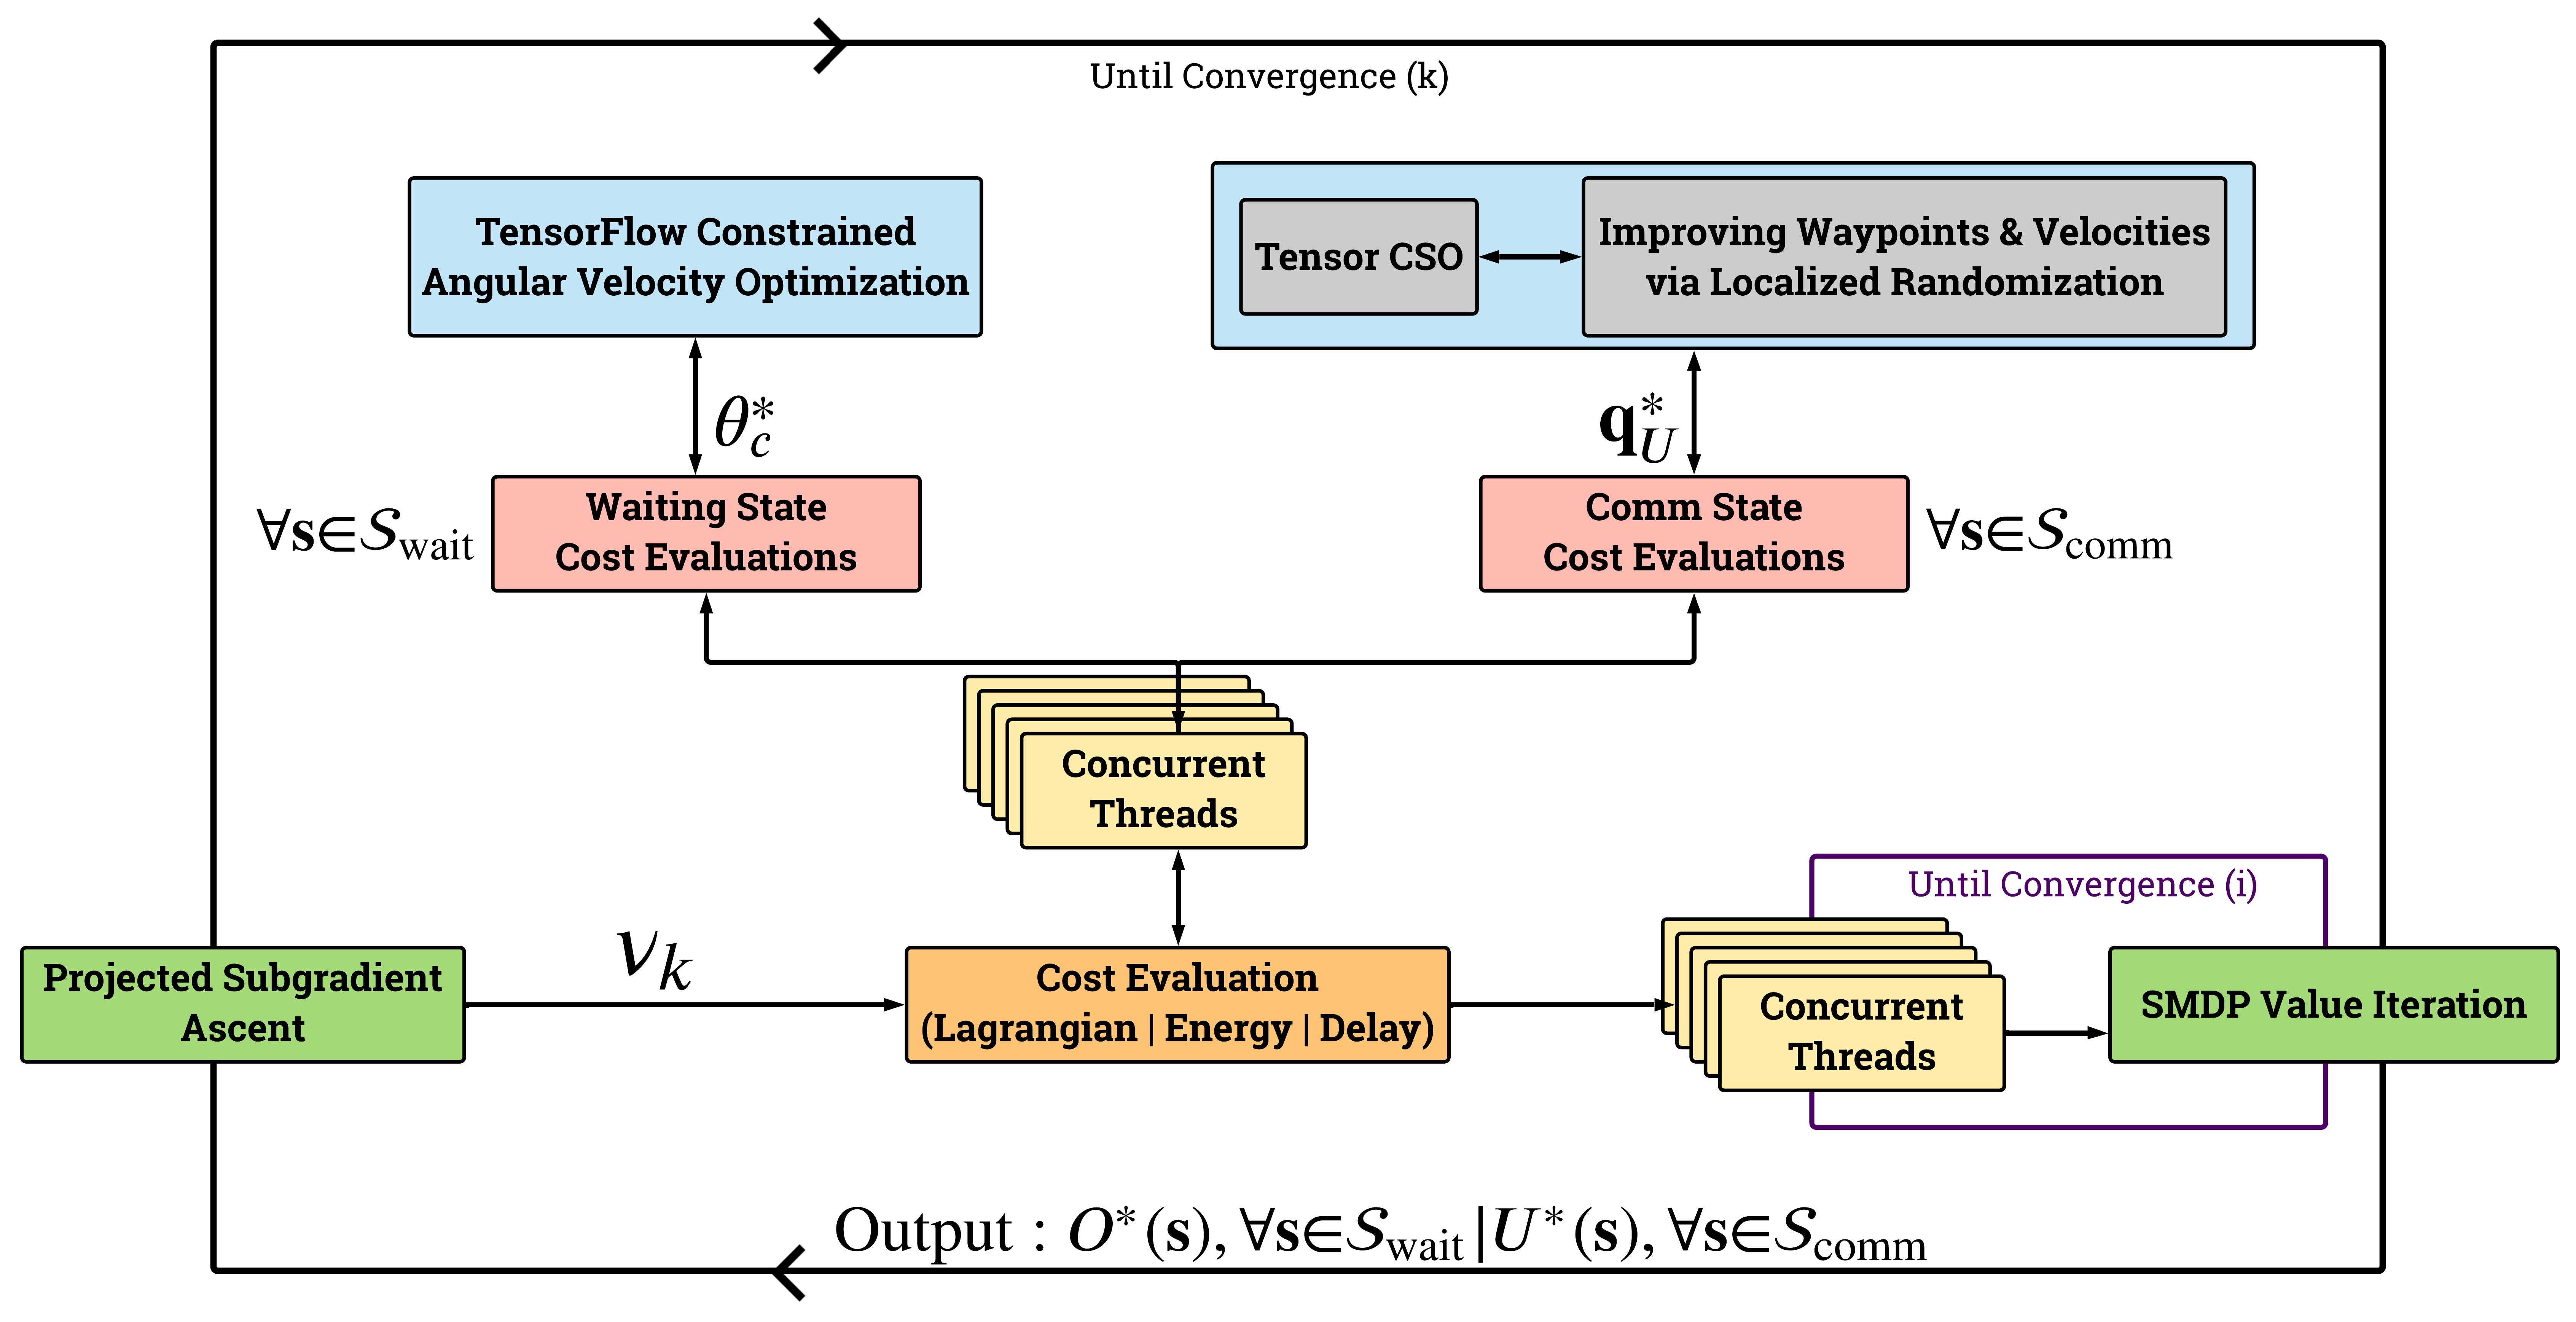
\includegraphics[width=0.9\linewidth]{figs/System_Flow_Chart.png}
    \caption{A depiction of the algorithmic flow inherent in our single-relay policy optimization process; computing accelerations via multi-threaded concurrency and distributed computing are also illustrated here.}
    \vspace{-8mm}
    \label{F3}
\end{figure}

\noindent{\textbf{Solution of (\textbf{P.0}) via the HCSO Method}}: To solve the problem with HCSO, we begin by randomly initializing a population of $M$-segment trajectory solutions (particles). Specifically, in the first call to the CSO algorithm \cite{CSO} (see Algorithm \ref{A4}) inside the HCSO framework, we initialize $N$ trajectory particles $\mathbf{p}_{1:N}{\triangleq}\mathbf{p}_{1},{\dots},\mathbf{p}_{N}$, with particle velocities $\mathbf{u}_{1:N}{\triangleq}\mathbf{u}_{1},{\dots},\mathbf{u}_{N}$, and $N$ UAV velocity particles $\mathbf{v}_{1:N}{\triangleq}\mathbf{v}_{1},{\dots},\mathbf{v}_{N}$, with particle velocities $\mathbf{w}_{1:N}{\triangleq}\mathbf{w}_{1},{\dots},\mathbf{w}_{N}$, imposing no trajectory structure in the first iteration. After the first CSO iteration, the resulting trajectory is interpolated to form a reference $2M$-segment trajectory, $\tilde{\mathbf{p}}{=}[\tilde{\mathbf{x}}_{1},{\dots},\tilde{\mathbf{x}}_{M{-}1}]^{T}$ and $\tilde{\mathbf{v}}{=}[\tilde{v}_{0},{\dots},\tilde{v}_{M{-}1}]^{T}$, with $M{\gets}2M$, so as to increase the resolution for the next iteration. The new population size is then reduced, $N{\gets}N{-}N_{\mathrm{red}}$, to lower the computational burden of CSO, and a new set of trajectories is generated randomly in a neighborhood around the reference trajectory. More precisely, the $m$th way-point, $\mathbf{x}_{m}{=}(x_{m},y_{m})$, of a new trajectory is generated as $\mathbf{x}_{m}{=}\tilde{\mathbf{x}}_{m}{+}(\chi_{m},\zeta_{m})$,
where the localized randomness in the new way-points is modeled using zero-mean Gaussian random variables, $\chi_{m},\zeta_{m}{\sim}\mathcal{N}\left(0,\varsigma\left(\Vert\tilde{\mathbf{x}}_{m{+}1}{-}\tilde{\mathbf{x}}_{m}\Vert^{2}{+}\Vert\tilde{\mathbf{x}}_{m{-}1}{-}\tilde{\mathbf{x}}_{m}\Vert^2\right)\right)$, with $\varsigma{>}0$ as a scaling factor, and the variance determined by the spread between neighboring reference trajectory way-points, incorporated due to the empirical observation that areas with clustered UAV way-points are the regions where the objective function \eqref{eq:Fhat} is sensitive to large variations. Likewise, the UAV velocity of the $m$th new trajectory segment is generated by $v_{m}{=}[\tilde{v}_{m}{+}\varkappa_{m}]^{[V_{\mathrm{low}},V_{\mathrm{max}}]}$
where $\varkappa_{m}{\sim}\mathcal{N}\left(0,\varepsilon\left(V_{\mathrm{max}}{-}V_{\mathrm{low}}\right)^{2}\right)$ induces randomness in the new velocity, $\varepsilon{>}0$ is a scaling factor, and $[\cdot]^{[V_{\mathrm{low}},V_{\mathrm{max}}]}{=}\mathrm{max}\left\{ \mathrm{min}\left\{\cdot,V_{\mathrm{max}}\right\},V_{\mathrm{low}}\right\}$ projects velocity $v_{m}$ to the feasible set. The variance is chosen due to the observation that the UAV velocities exhibit consistent convergence with CSO much faster than the trajectory way-points and are less sensitive to random initializations.

\begin{algorithm}[t]
\caption{Hierarchical Competitive Swarm Optimization: HCSO($\mathbf{s};U(\mathbf{s})$)}\label{A3}
    \begin{algorithmic}[1]
    	\State \textbf{Initialization}: Randomly initialize UAV way-points $\mathbf{p}_{1:N}$ and velocities $\mathbf{v}_{1:N}$.
    	\vspace{.2cm}
    	\While{$M{\leq}M_{\mathrm{max}}$}
    	    \vspace{.2cm}
    		\State Obtain $M$-segment trajectory: $(\mathbf{p}^{*},\mathbf{v}^{*})=\mathrm{CSO}(\mathbf{p}_{1:N},\mathbf v_{1:N},N,M)$ (see Algorithm \ref{A4}).
    		\vspace{.2cm}
    		\State Increase $M{\gets}2M$; interpolate to form reference trajectory: $(\tilde{\mathbf{p}},\tilde{\mathbf{v}}){=}\mathrm{interp}(\mathbf{p}^{*},\mathbf{v}^{*},M)$.
    		\vspace{.2cm}
    		\State Reduce population size $N{\gets}N{-}N_{\mathrm{red}}$.
    		\vspace{.2cm}
    		\For{$n_{1}{=}1,2,{\dots},N$}
    		    \vspace{.2cm}
    			\For{$n_{2}{=}1,2,{\dots},M{-}1$}
    			    \vspace{.2cm}
    			    \State $\mathbf{x}_{n_{2}}{=}\tilde{\mathbf{x}}_{n_{2}}{+}(\chi_{n_{2}},\zeta_{n_{2}})$ with $\tilde{\mathbf{x}}_{n_{2}}{\in}(\tilde{x}_{n_{2}},\tilde{y}_{n_{2}})$ in $\tilde{\mathbf{p}}$; $\mathbf{x}_{n_{2}}{\in}\mathbf{p}_{n_{1}}$.
    				\vspace{.2cm}
    			\EndFor
    			\vspace{.2cm}
    			\For{$n_{3}{=}0,{\dots},M-1$}
    			    \vspace{.2cm}
    			    \State $\tilde{v}_{n_{3}}{=}[\tilde{v}_{n_{3}}{+}\varkappa_{n_{3}}]^{[V_{\mathrm{low}},V_{\mathrm{max}}]}$ with $\tilde{v}_{n_{3}}{\in}\tilde{\mathbf{v}}$; $v_{n_{3}}{\in}\mathbf{v}_{n_{1}}$.
    				\vspace{.2cm}
    			\EndFor
    			\vspace{.2cm}
    			\State Update new swarm particle $\mathbf p_{n_{1}}{\gets}[\mathbf{x}_{1},{\dots},\mathbf{x}_{M{-}1}]^{T}$ and $\mathbf{v}_{n_{1}}{\gets}[v_{0},{\dots},v_{M{-}1}]^{T}$.
    			\vspace{.2cm}
    		\EndFor
    		\vspace{.2cm}
    	\EndWhile
    \end{algorithmic}
\end{algorithm}

The HCSO scheme is outlined in Algorithm \ref{A3}. Line $1$ initializes $N$ random $M$-segment UAV trajectories; line $3$ obtains an $M$-segment trajectory with CSO \cite{CSO} (Algorithm \ref{A4}); line $4$ doubles the trajectory resolution and interpolates the CSO output to a $2M$-segment reference trajectory; lines $8$ and $11$ generate random trajectories in a neighborhood of the reference trajectory, $(\tilde{\mathbf p}, \tilde{\mathbf v})$. The process repeats until the trajectory resolution equals a desired value.

\begin{algorithm}[t]
\caption{Competitive Swarm Optimization: $(\mathbf{p}^{*},\mathbf{v}^{*}){=}\mathrm{CSO}\left(\mathbf{p}_{1:N}(0),\mathbf{v}_{1:N}(0),N,M\right)$}\label{A4}
    \begin{algorithmic}[1]
    	\State \textbf{Initialization:} $k{=}0$, particle velocities $\mathbf{u}_{1:N}(0)$ and $\mathbf{w}_{1:N}(0)$ for $\mathbf{p}_{1:N}(0)$ and $\mathbf{v}_{1:N}(0)$.
    	\vspace{.2cm}
    	\Repeat
    	    \vspace{.2cm}
    		\State Shuffle particle indices with a random permutation: $t(i):\{1,{\dots},N\}{\mapsto}\{1,{\dots},N\}$.
    		\vspace{.2cm}
    		\For{$j{=}1,3,5,{\dots},N{-}1$}
    		    \vspace{.2cm}
    			\If{$\hat{f}(\mathbf{p}_{t(j)}(k),\mathbf{v}_{t(j)}(k)){\leq}\hat{f}(\mathbf{p}_{t(j{+}1)}(k),\mathbf{v}_{t(j{+}1)}(k))$}
    			    \vspace{.2cm}
    				\State $(\mathbf{p}^{w},\mathbf{v}^{w}){=}(\mathbf{p}_{t(j)}(k), \mathbf{v}_{t(j)}(k))$; $(\mathbf{p}^{l},\mathbf{v}^{l}){=}(\mathbf{p}_{t(j{+}1)}(k), \mathbf{v}_{t(j{+}1)}(k))$
    				\vspace{.2cm}
    				\State $j_{\mathrm{win}}{=}t(j)$; $j_{\mathrm{los}}{=}t(j{+}1)$.
    				\vspace{.2cm}
    			\Else
    			    \vspace{.2cm}
    				\State $(\mathbf{p}^{w},\mathbf{v}^{w}){=}(\mathbf{p}_{t(j{+}1)}(k), \mathbf{v}_{t(j{+}1)}(k))$; $(\mathbf{p}^{l},\mathbf{v}^{l}){=}(\mathbf{p}_{t(j)}(k), \mathbf{v}_{t(j)}(k))$
    				\vspace{.2cm}
    				\State $j_{\mathrm{win}}{=}t(j{+}1)$; $j_{\mathrm{los}}{=}t(j)$.
    				\vspace{.2cm}
    			\EndIf
    			\vspace{.2cm}
    			\State Pass the winner to next iteration: $(\mathbf{p}_{j_{\mathrm{win}}}(k{+}1),\mathbf{v}_{j_{\mathrm{win}}}(k{+}1)){\gets}(\mathbf{p}^{w},\mathbf{v}^{w})$.
    			\vspace{.2cm}
    			\State Update loser particle velocities $(\mathbf{u}_{j_{\mathrm{los}}}(k{+}1),\mathbf{w}_{j_{\mathrm{los}}}(k{+}1))$ using \eqref{eq:UpdtU} and \eqref{eq:UpdtW}.
    			\vspace{.2cm}
    			\State Update loser particles $(\mathbf{p}_{j_{\mathrm{los}}}(k{+}1),\mathbf{v}_{j_{\mathrm{los}}}(k{+}1))$ using \eqref{eq:UpdtPV}.
    			\vspace{.2cm}
    		\EndFor
    		\vspace{.2cm}
    		\State $k{\gets}k{+}1$.
    		\vspace{.2cm}
    	\Until{maximum number of cost function evaluations performed.}
    	\vspace{.2cm}
    	\newline
    	\Return{$(\mathbf{p}^{*},\mathbf{v}^{*}){=}\argmin\{\hat{f}(\mathbf{p}_{i}(k),\mathbf{v}_{i}(k)),{\forall}i{=}1,{\dots},N\}$}
    \end{algorithmic}
\end{algorithm}

The CSO scheme follows \cite{CSO} and is shown in Algorithm \ref{A4}. During the $k$th iteration inside CSO, the $N$ particles are randomly grouped into $\frac{N}{2}$ pairwise competitions. For both members of a pair, the penalized objective function in \eqref{eq:Fhat} is calculated; the winner of the competition is passed onto the $(k{+}1)$th iteration of CSO, and the loser is modified by learning from the winner. Let $j_{\mathrm{win}}, j_{\mathrm{los}}{\in}\{1,{\dots},N\}$ denote the indices of the winner and the loser from the population during the $j$th pairwise competition, in the $k$th iteration of CSO. Accordingly, we denote the winner and loser particles by $(\mathbf{p}^{w},\mathbf{v}^{w})$ and $(\mathbf{p}^{l},\mathbf{v}^{l})$, respectively. The loser particle and its velocities are updated as
\begin{align}
	&\mathbf u_{j_{\mathrm{los}}} (k+1) = r_{j,1} (k) \mathbf u^l + r_{j,2}(k) \left( \mathbf p^w - \mathbf p^l \right) + \omega \cdot r_{j,3}(k) \left( \bar{\mathbf p}(k) - \mathbf p^l \right),\label{eq:UpdtU}\\
	&\mathbf w_{j_{\mathrm{los}}} (k+1) = r_{j,1} (k) \mathbf w^l + r_{j,2}(k) \left( \mathbf v^w - \mathbf v^l \right) + \omega \cdot r_{j,3}(k) \left( \bar{\mathbf v}(k) - \mathbf v^l \right),\text{ and }\label{eq:UpdtW}\\
	&\mathbf p_{j_{\mathrm{los}}} (k+1) = \mathbf p^l + \mathbf u_{j_{\mathrm{los}}} (k+1), \;\; \mathbf v_{j_{\mathrm{los}}} (k+1) = \left[ \mathbf v^l + \mathbf w_{j_{\mathrm{los}}} (k+1) \right]^{[V_{\mathrm{low}},V_{\mathrm{max}}]},\label{eq:UpdtPV}
\end{align}
where $r_{j,1}(k),r_{j,2}(k),\text{ and }r_{j,3}(k)$ are independent uniform random variables on the interval $[0,1]$; $\bar{\mathbf{p}}(k)$ and $\bar{\mathbf{v}}(k)$ are the global means of the UAV way-point and velocity particles in the $k$th CSO iteration; and $\omega$ is a scale parameter for the degree of influence of $\bar{\mathbf{p}}(k)$ and $\bar{\mathbf{v}}(k)$.

\noindent{\textbf{Computing Accelerations}}: In order to further boost policy training times, and turn our proposed scheme into a scalable and tractable solution, we incorporate efficient design methodologies for the implementation of Algorithms \ref{A1}, \ref{A2}, \ref{A3}, and \ref{A4} in software. Leveraging a fully-vectorized implementation in TensorFlow \cite{TF1}, we perform concurrent executions (via Python worker threads) of appropriately disassociated program blocks. These concurrent executions exploit distributed computing capabilities available at our disposal via context-based device placement over CUDA-capable GPUs and just-in-time accelerated CPUs \cite{TF2}. The computing accelerations outlined above facilitate significant improvements in policy convergence times, as discussed in Sec. \ref{S6}. A multi-relay extension to MAESTRO is described next.
\vspace{-3mm}


\section{MAESTRO-X: An Extension to UAV Swarms via Supplementary Heuristics}\label{S5}
\vspace{-2mm}

\begin{figure} [t]
    \centering
    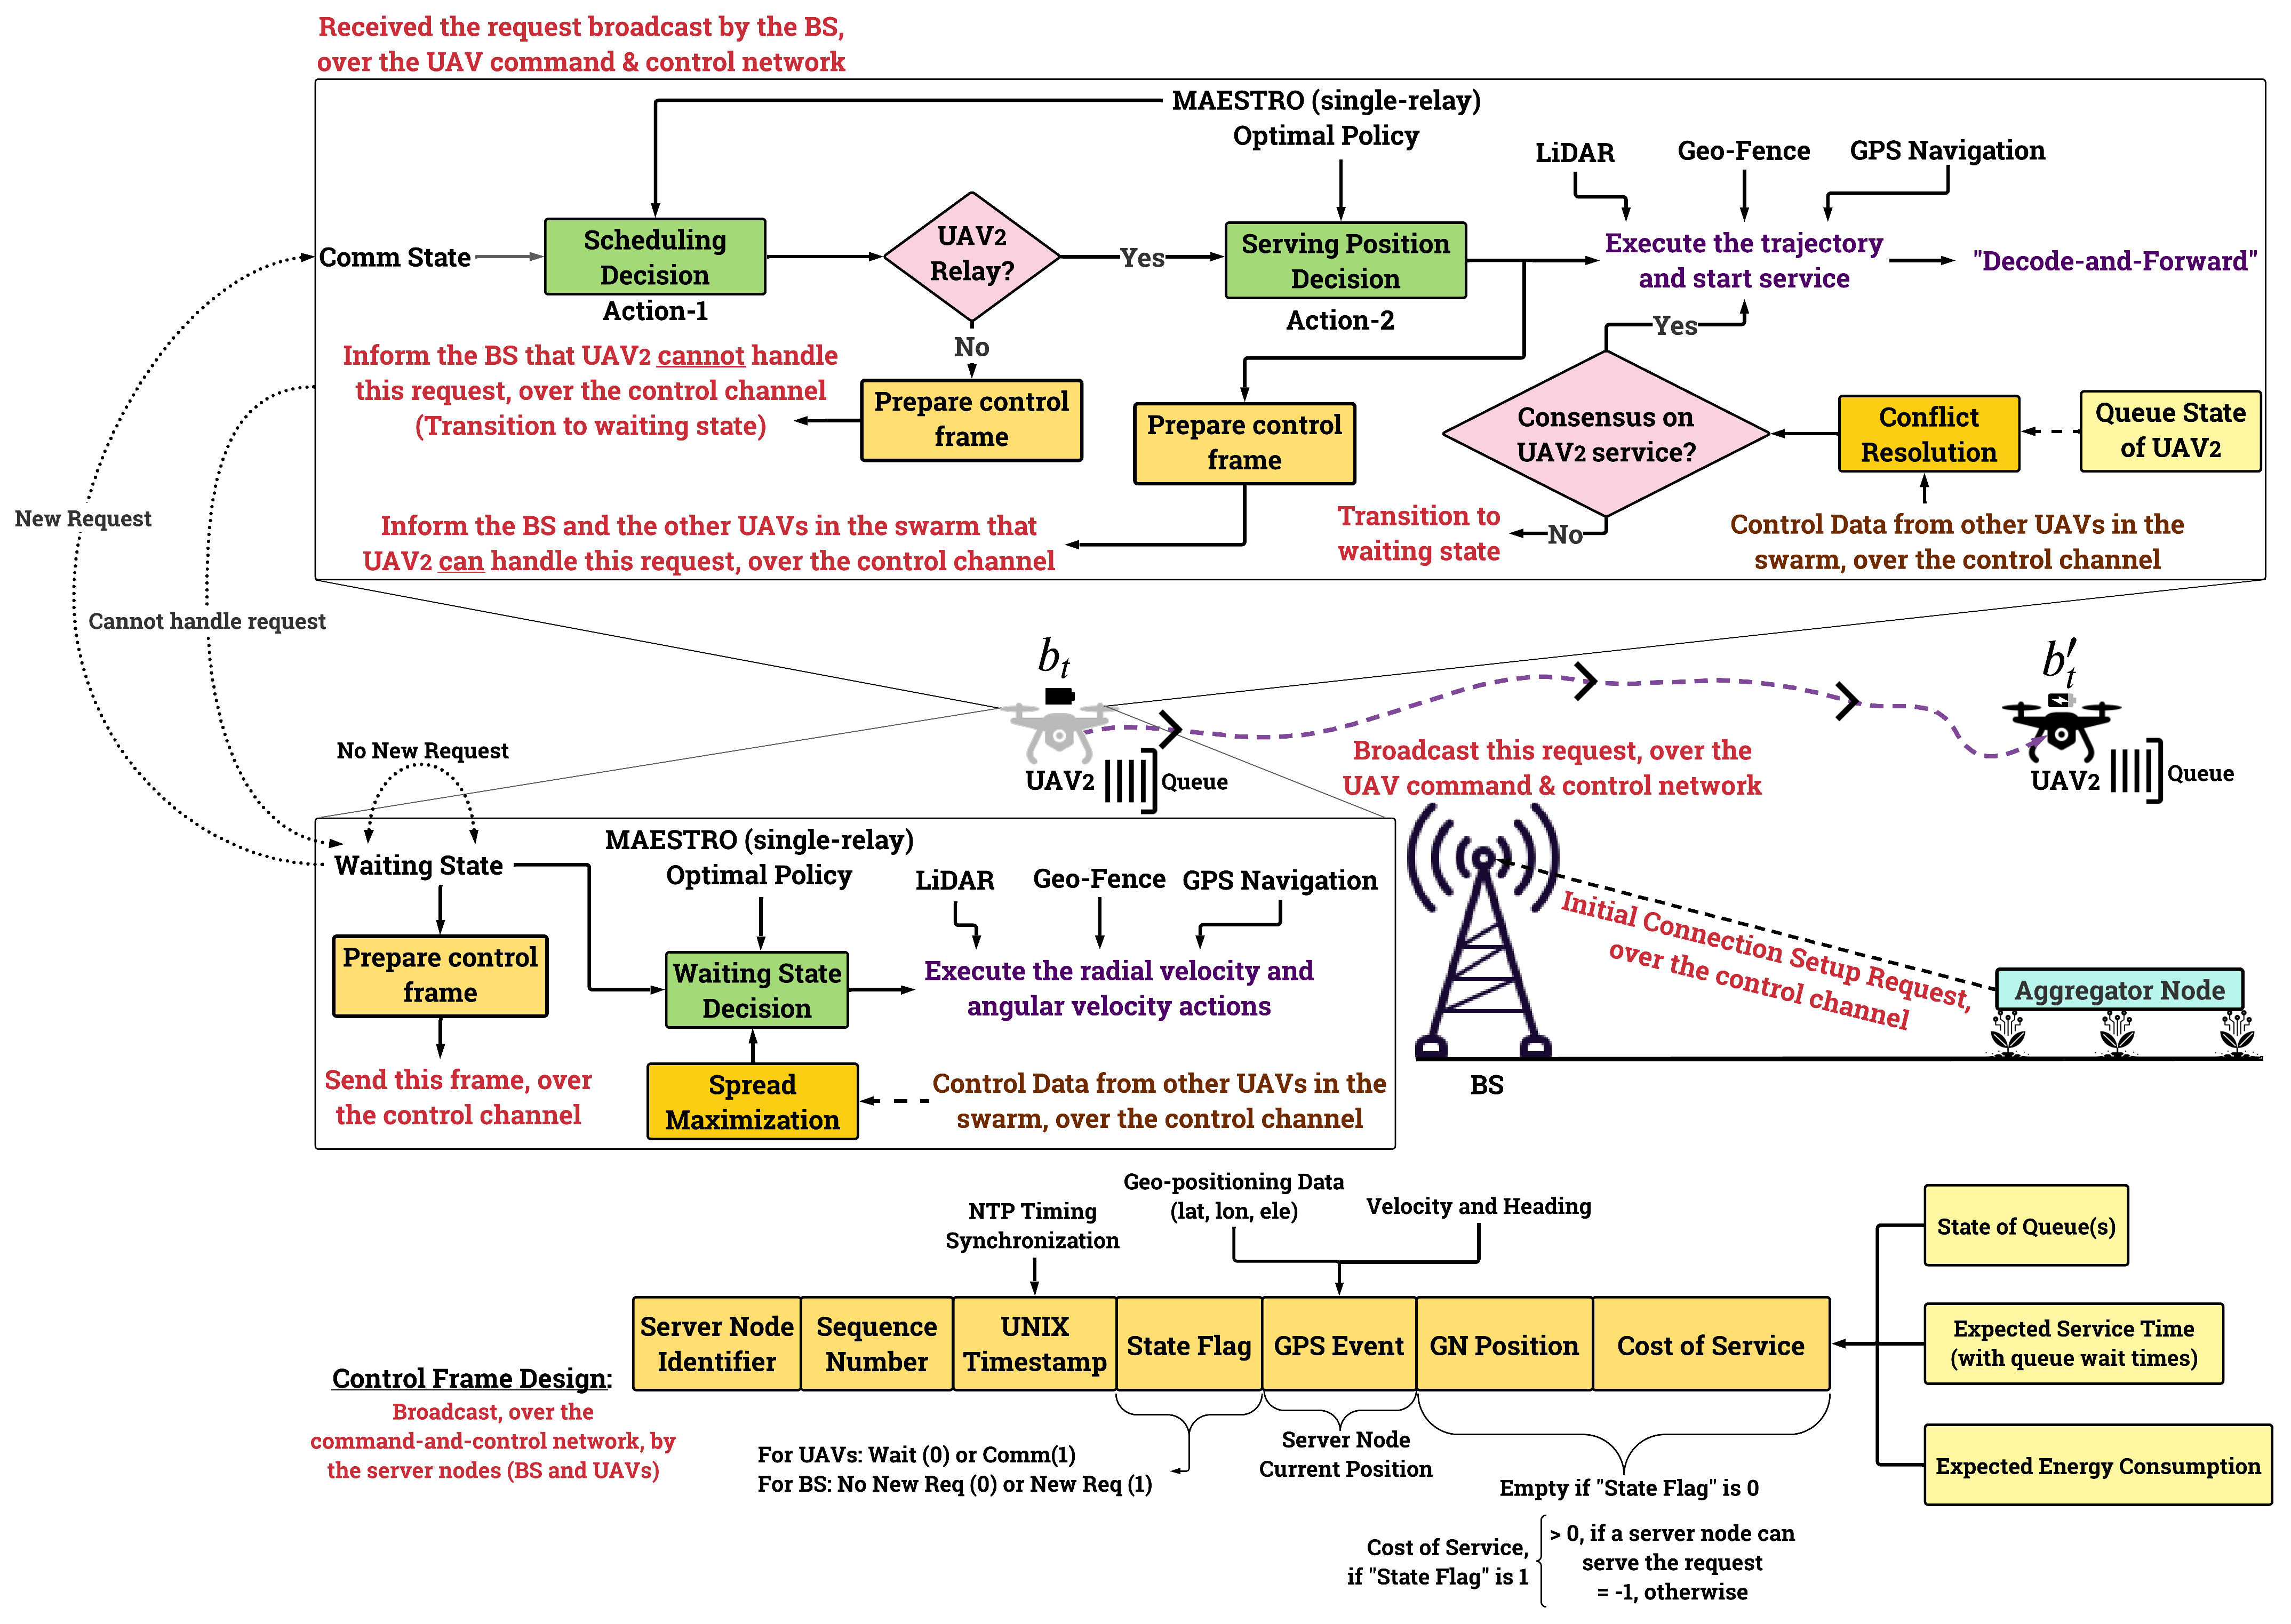
\includegraphics[width=0.9\linewidth]{figs/System_Operation.png}
    \caption{The study of a hybrid wireless network augmented by a swarm of UAV relays in precision agriculture: an illustration outlining the sequence of operations under MAESTRO-X that occur at $\text{UAV}_{2}$ in the swarm; our control frame structure is also depicted here.}
    \vspace{-8mm}
    \label{F4}
\end{figure}

In this section, we remove the specializations considered for our single-relay construction in Sec. \ref{S3}, and extend the optimal scheduling and trajectory optimization framework (MAESTRO) developed in Secs. \ref{S3} and \ref{S4} to our generalized hybrid wireless network model of $N_{U}$ UAV relays in the swarm. MAESTRO's eXtension, termed MAESTRO-X, constitutes augmentations to the multiscale optimal \emph{waiting} and \emph{communication} policy obtained via SMDP value iteration (within which HCSO determines the service trajectory). Depicting an example scenario of serving data traffic generated by an aggregation of soil sensors in precision agriculture, Fig. \ref{F4} illustrates the control flow of MAESTRO-X---in particular, the operations of $\mathrm{UAV}_{2}$. Along with a fully-connected mesh network overlaid over the BS and the UAV swarm for command-and-control operations, enhancements to MAESTRO include spread maximization (in the \emph{waiting} phase) and conflict resolution (in the \emph{request scheduling} phase). After these heuristics are embedded into MAESTRO, the modified policy is replicated across the swarm, resulting in an implementation centered around multiple decoupled executions driven by a single optimal policy.

\noindent{\textbf{Policy Replication}}: Post policy convergence via the algorithms detailed in Secs. \ref{S3} and \ref{S4}, the optimal behavior of our multiscale adaptive framework developed for the automation of single-relay operations (i.e., MAESTRO) is stored in a database: an organized collection of key-value pairs. Staying true to the SMDP state space construction, this database is partitioned into two lookup tables. The \emph{waiting} phase lookup table constitutes the SMDP waiting states as the keys and their associated radial and angular velocity actions as the corresponding values. Similarly, the \emph{request scheduling} phase lookup table constitutes the SMDP communication states as the keys and their associated UAV service trajectories and service times (for both the BS and the UAVs) as the corresponding values. This optimal policy database is then replicated to the BS as well as all the UAVs in the swarm. During their operations, these server nodes (BS + UAVs) lookup the optimal actions vis-à-vis their current states---and, with further enhancements such as collaboration message exchanges, spread maximization (in the \emph{waiting} phase) and consensus-driven conflict resolution (in the \emph{request scheduling} phase)---execute optimal actions that have been augmented to orchestrate swarm operations in a decentralized fashion.

\noindent{\textbf{Command-and-Control Network}}: Truly decentralized and coordinated operations of the UAV relays in the swarm necessitates the need for a control network over which the server nodes can collaborate to $1$) ensure collision-free movements among the UAVs\footnote{We reasonably assume that the UAVs are equipped with a LiDAR-based obstacle avoidance system: when an obstacle is detected during the UAV's flight, a fallback guidance system on-board navigates the UAV around the obstacle. The incorporation of obstacles and No-Fly-Zones into our model will be tackled in future works.}; $2$) facilitate consensus-driven system-wide decisions on the best server to handle a GN uplink transmission request that originated in the cell, thereby mitigating the additional computational complexity endured by joint/combined multi-relay optimization frameworks \cite{DDQN, CSCA-ADMM}; and $3$) guarantee resilient fault-tolerant operations by setting-up fallback mechanisms to handle UAV-failures. We designate the band-edges of the allocated spectrum as control channels, over which the server nodes in the cell exchange short frames: the structure of a control frame in MAESTRO-X is shown in Fig. \ref{F4}. A fully-connected distributed mesh topology (employing these designated control channels) overlaid over the BS and the UAV swarm constitutes the design of our command-and-control network. Since each UAV relay in the swarm possesses the same optimal \emph{waiting} and \emph{communication} state policies, we introduce spread maximization (in the \emph{waiting} states) and conflict resolution heuristics (in the \emph{communication} states) to cooperatively handle their operations. These heuristics are discussed next. 

\noindent{\textbf{Spread Maximization}}: To efficiently position and prime the idle UAVs for a potential new GN request originating in the cell, in the \emph{waiting} states, a UAV relay in the swarm, in addition to executing the optimal action (corresponding to its current radius level), determines the direction of angular motion (clockwise or counter-clockwise) based on our spread maximization heuristic---wherein each UAV relay in the \emph{waiting} state and in a radius level with zero radial velocity, executes either positive (counter-clockwise) or negative (clockwise) angular movements in order to maximize the minimum distance among them. These coordinated movements among the UAVs is made possible through periodic exchanges of control frames over the command-and-control network. Studying this frame structure in Fig. \ref{F4}, we note that for waiting states, `State Flag' is set to $0$, and the `GN Position' and `Cost of Service' fields are empty. The `GPS Event' field constitutes the most crucial component in a \emph{waiting} state control frame: UAVs in the \emph{waiting} state extract the positional information of their peers from this field, and apply a \emph{maximize-the-minimum-distance} heuristic over other UAVs which are \emph{waiting} in the same radius level. This methodology ensures that a suitable spread is maintained among the idle UAVs, in order to facilitate faster response times when a new uplink request is generated. 

\noindent{\textbf{Consensus-driven Conflict Resolution}}: When a new uplink transmission request originates in the cell, the UAVs already serving a GN continue to do so, i.e., they do no participate in the consensus-driven conflict resolution process. These relays, termed `unavailable' under this context, transition into their corresponding \emph{waiting} states upon service completion. On the other hand, UAVs in the \emph{waiting} states transition into their respective \emph{communication} states. The BS along with these relays are deemed to be `available'. These `available' server nodes exchange collaboration messages over the command-and-control network. The structure of this control frame is depicted in Fig. \ref{F4}: `State Flag' is set to $1$, the `GN position' field is populated with the originating position of the uplink transmission request under consideration, and the `Cost of Service' field constitutes a weighted sum of the request service time (communication service + queue wait) and the necessary energy consumption to serve it. These values on communication service times and energy consumption are obtained from the policy lookup table (whose design was discussed earlier in this section); the queueing latencies at these server nodes are obtained by modeling an M/G/$N_{B}$ queueing system at the BS and an M/G/$1$ queueing system at each UAV relay. Note that the BS' energy consumption for serving a GN request is set to $0$. Upon sharing these metrics with each other, these nodes arrive at a consensus on the most efficient choice (vis-à-vis service delay and energy consumption) to successfully handle the active GN request. Next, we chronicle our simulation setup and the corresponding results from our numerical evaluations of both MAESTRO and MAESTRO-X.
\vspace{-4mm}


\section{The Simulation Setup and Numerical Evaluations}\label{S6}

\begin{table}
\scriptsize
\centering
    \begin{tabular}{|p{2cm}|p{8cm}|p{5.2cm}|}
    \hline
    {\bf{Notation(s)}} & {\bf{Physical Meaning/Description}} & {\bf{Simulation Value(s)}} \\
    \hline
    $a$ & Radius of the cell & \qty[mode=text]{1000}{\meter}\\ 
    \hline
    $(x_{B}, y_{B})$ & Rectangular coordinates of the BS & (\qty[mode=text]{0}{\meter}, \qty[mode=text]{0}{\meter})\\ 
    \hline
    $H_{\text{B}}$ & GPS ellipsoidal height of the BS antennae & \qty[mode=text]{80}{\meter}\\
    \hline
    $H_{\text{U}}$ & GPS ellipsoidal height of the antennae on-board the UAV Relay(s) & \qty[mode=text]{200}{\meter}\\
    \hline
    $N_{\text{G}}$ & Number of GNs in the cell & \num{300}\\
    \hline
    $N_{\text{U}}$ & Number of UAV relays in the formulation & [\num{1}, \num{2}, \num{3}]\\
    \hline
    $\lambda_{G}$ & GN distribution density in the cell & \qty[mode=text]{9.55e-6} {GNs\per\meter^{2}}\\
    \hline
    $L$ & Data payload size to be serviced for each GN request & [\num{1}, \num{10}, \num{100}] \unit{Mb}\\
    \hline
    $\lambda_{R|G}$ & Rate of the Poisson arrival process for requests originating at each GN & [\num{5.6e-4}, \num{1.1e-4}, \num{1.9e-5}] \unit{req\per GN \per\second}\\
    \hline
    $\lambda_{R}$ & Rate of the Poisson arrival process for requests per unit area & [\num{5.3e-9}, \num{1.1e-9}, \num{1.8e-10}] \unit{req\per\second\per\meter^{2}}\\
    \hline
    $\Lambda$ & Overall rate of requests originating in the cell & [\num{1.7e-2}, \num{3.3e-3}, \num{5.6e-4}] \unit{req\per\second}\\
    \hline
    $\Delta_{0}$ & UAV relay(s) waiting-state action execution time-frame & [\num{4.35}, \num{21.79}, \num{130.52}] \unit{\second}\\
    \hline
    $U_{\text{tip}}$ & Rotor blade tip velocity in the rotary-wing UAV & \qty[mode=text]{200}{\meter\per\second}\\
    \hline
    $v_{0}$ & Mean rotor-induced velocity in the rotary-wing UAV & \qty[mode=text]{7.2}{\meter\per\second}\\
    \hline
    $v_{\text{max}}$ & Maximum forward flying velocity constraint value for the UAV relay(s) & \qty[mode=text]{55}{\meter\per\second}\\
    \hline
    $P_{1}$ & UAV mobility power profile constant vis-à-vis the blade profile & \qty[mode=text]{580.65}{\watt}\\
    \hline
    $P_{2}$ & UAV mobility power profile constant vis-à-vis the induced velocity & \qty[mode=text]{790.6715}{\watt}\\
    \hline
    $P_{3}$ & UAV mobility power profile constant vis-à-vis parasite terms & \qty[mode=text]{0.0073}{\kilogram\per\meter}\\
    \hline
    $P_{\text{avg}}$ & Average mobility power constraint value for the UAV relay(s) & $\{1.0{+}j(0.1),{\forall}j{\in}\{0,1,2,\dots,10\}\}$ \unit{\watt}\\
    \hline
    $B$ & Bandwidth of each channel used for GB, GU, and UB links & \qty[mode=text]{5}{\mega\hertz}\\
    \hline
    $\gamma_{\text{GB}}{=}\gamma_{\text{GU}}{=}\gamma_{\text{UB}}$ & The SNR at a reference Tx-Rx distance of \qty[mode=text]{1}{\meter} & \qty[mode=text]{40}{\decibel}\\
    \hline
    $\alpha$ & Path-loss exponent for LoS links & \num{2}\\
    \hline
    $k_{1}$ & Radio environment coefficient of the Rician LoS $K$-factor & \num{1}\\
    \hline
    $k_{2}$ & Radio environment coefficient of the Rician LoS $K$-factor & \num{0.051}\\
    \hline
    $\tilde{\alpha}$ & Path-loss exponent for NLoS links & \num{2.8}\\
    \hline
    $\kappa$ & Additional NLoS attenuation factor & \num{0.2}\\
    \hline
    $z_{1}$ & Radio environment coefficient for LoS/NLoS probability evaluation & \num{9.61}\\
    \hline
    $z_{2}$ & Radio environment coefficient for LoS/NLoS probability evaluation & \num{0.16}\\
    \hline
    $R_{\text{sp}}$ & Number of UAV radial velocity levels & \num{25}\\
    \hline
    $N_{\text{sp}}$ & Number of radius levels in the cell & \num{25}\\
    \hline
    $\epsilon_{Z}$ & Bisection method tolerance for rate adaptation & \num{1e-10}\\
    \hline
    $\alpha_{\theta_{c}}$ & Learning rate for UAV angular velocity optimization & \num{1e-4}\\
    \hline
    $\epsilon_{\theta_{c}}$ & Termination threshold for UAV angular velocity optimization & \num{1e-10}\\
    \hline
    $\delta$ & Termination threshold for SMDP Value Iteration & \num{1e-3}\\
    \hline
    $\epsilon_{\text{PF}}$ & Primal feasibility threshold in projected sub-gradient ascent & \num{1e-3}\\
    \hline
    $\rho_{0}$ & Initial dual step-size in projected sub-gradient ascent & \num{1}\\
    \hline
    $\epsilon_{\text{DI}}$ & Dual convergence threshold in projected sub-gradient ascent & \num{1e-3}\\
    \hline
    $\epsilon_{\text{CS}}$ & Complementary slackness threshold in projected sub-gradient ascent & \num{0.1}\\
    \hline
    $N_{\text{max}}$ & Maximum number of cost function evaluations in CSO & \num{1000}\\
    \hline
    $M$ & Initial number of trajectory segments in HCSO & \num{16}\\
    \hline
    $M_{\text{max}}$ & Maximum number of trajectory segments in HCSO & \num{256}\\
    \hline
    $N$ & Initial number of trajectory and velocity particles in HCSO & \num{400}\\
    \hline
    $\zeta{=}\epsilon{=}\omega$ & Scale parameters in HCSO & \num{1}\\
    \hline
    \end{tabular}
\caption{Simulation Parameters}\label{T2}
\vspace{-10mm}
\end{table}

As outlined in Table \ref{T2}, in our numerical evaluations of MAESTRO and MAESTRO-X, we use a channel bandwidth of $B=$ \qty[mode=text]{5}{\mega\hertz}; for all links, NLoS attenuation constant $\kappa=$ \qty[mode=text]{0.2}{}, $1$-meter reference SNR $\frac{\beta_{0}P}{\sigma^{2}\Gamma}=$ \qty[mode=text]{40}{\decibel}, LoS path-loss exponent $\alpha=$ \qty[mode=text]{2}{}, NLoS path-loss exponent $\tilde{\alpha}=$ \qty[mode=text]{2.8}{}, Rician $K$-factor parameters $k_{1}=$ \qty[mode=text]{1}{} and $k_{2}=$ \qty[mode=text]{0.05}{} \cite{Rician}, and LoS probability parameters $z_{1}=$ \qty[mode=text]{9.61}{} and $z_{2}=$ \qty[mode=text]{0.16}{} \cite{OptimalAltitude}; UAV height $H_{U}=$\qty[mode=text]{200}{\meter}; BS antenna height $H_{B}=$\qty[mode=text]{80}{\meter}; maximum UAV velocity $V_{\mathrm{max}}=$ \qty[mode=text]{55}{\meter\per\second}; and cell radius $a=$ \qty[mode=text]{1000}{\meter}. The UAV power consumption model uses the relationship described in \eqref{eq:Power} and the parameters listed Table \ref{T2} (according to the studies detailed in \cite{SCA}). We solve an approximation of problem \eqref{eq:PolDecomp} by discretizing the state and action spaces and applying linearly-interpolated value iteration. The dual variable yields meaningful results for $\nu{\in}[0,\frac{1}{P_{\mathrm{avg}}}]$, thus by solving the problem for $20$ values in the interval, an approximation to the maximum $g(\nu^*)$, emerges. We discretize the states with $N_{\mathrm{sp}}=$ \qty[mode=text]{25}{} equispaced radii values, with $12$ GNs in each level; and $R_{\mathrm{sp}}=$ \qty[mode=text]{25}{} equispaced radial velocity actions for $v_r{\in}\{-V_{\mathrm{max}},{\dots},V_{\mathrm{max}}\}$. Lastly, $\Delta_{0}$ is chosen to satisfy $e^{-\Lambda\Delta_{0}}=$ \qty[mode=text]{0.93}{}, so that it is unlikely to receive two or more requests in $\Delta_{0}$.

\bk{\underline{In progress}: To benchmark HCSO against SCA and non-hierarchical CSO for solving the inner Lagrangian cost metric, $\ell_{\nu}^{*}(s;U(s))$, we choose state $s{=}(800,500,\frac{\pi}{4})$ [m,m,rad], end radius $U(s)=$ \qty[mode=text]{700}{\meter}, target average power $P_{\mathrm{avg}}=$ \qty[mode=text]{1.2}{\kilo\watt}, and data payload $10$ Mb. For HCSO (Algorithm \ref{A3}), with the initial trajectory size $M=$ \qty[mode=text]{16} and the maximum allowed trajectory size $M_{\mathrm{max}}=$ \qty[mode=text]{256}, we make $4$ calls to CSO, doubling the trajectory resolution each iteration as $M_{\mathrm{HCSO}}(i){=}2^{i{+}1}$, for $i{=}1,{\dots},4$; we decrease the swarm size after each CSO call as $N_{\mathrm{HCSO}}(i){=}400{-}20i$, for $i{=}1,{\dots},4$. In Fig. \ref{F5}, we observe that the HCSO realizations converge up to $21{\times}$ faster in time. Thus, HCSO is preferable to SCA for time efficiency, considering that ${\approx}10,000$ realizations must be solved with the SMDP discretization for fixed $\nu$ and $P_{\mathrm{avg}}$. Finally, Fig. \ref{F5} shows that HCSO finds solutions that reduce the objective function value by up to $42\%$, when compared to non-hierarchical CSO.} 

Furthermore, as shown in Fig. \ref{F6}, bench-marking our MAESTRO-X framework against both model-based \cite{CSCA-ADMM} and model-free \cite{DDQN} solutions in the state-of-the-art, we observe that the decoupled policy replication across the swarm---with suitable supplementary heuristics---ensures that our solution constitutes a practically feasible formulation even with higher-degrees of scaling in the number of UAVs in the swarm. The Constrained Successive Convex Approximation (CSCA) wrapped Alternating Direction Method-of-Multipliers (ADMM) approach in \cite{CSCA-ADMM} and the Double Deep-Q Network (DDQN) with Combined Experiential Replay (CER) approach in \cite{DDQN} involve prohibitively large policy convergence times when the number of the UAVs in the swarm is scaled beyond $N_{U}{=}5$ and $N_{U}{=}6$, respectively. All implementations are in Python, and this bench-marking is performed on a compute node with $2{\times}$ $64$-core AMD EPYC Milan 7763 CPUs, $16{\times}$ $64$ GB DDR$4$ memory, and $4{\times}$ NVIDIA A$100$ GPUs with $40$ GB VRAM each. The CSCA-ADMM solution in \cite{CSCA-ADMM} suffers poor bench-marking performance relative to MAESTRO-X due to a joint multi-UAV construction involved in its CVXPY\footnote{CVXPY: A library for solving convex optimization problems in Python.}-SCS\footnote{Split Conic Solver (SCS): The optimizer employed within our CVXPY implementation of \cite{CSCA-ADMM}.} implementation; the DDQN-CER\footnote{A TensorFlow-Keras implementation, the source code for which was made available on \href{https://github.com/hbayerlein/uav_data_harvesting.git}{GitHub} \cite{DDQN}.} solution in \cite{DDQN} demonstrates larger policy convergence times relative to MAESTRO-X due to an underlying model-free formulation, in addition to an MDP construction that considers combined multi-UAV state and action spaces. On the other hand, the decoupled policy executions in MAESTRO-X mitigates the computational overhead encountered by the joint/combined multi-UAV constructions in \cite{CSCA-ADMM} and \cite{DDQN}; moreover, multi-threading concurrency (128 software threads per CPU) and distributed computing (over the $2$ CPUs and $4$ GPUs) facilitate accelerations in MAESTRO's policy convergence.

\begin{figure}[t]
	\begin{subfigure}{0.49\textwidth}
		\centering
		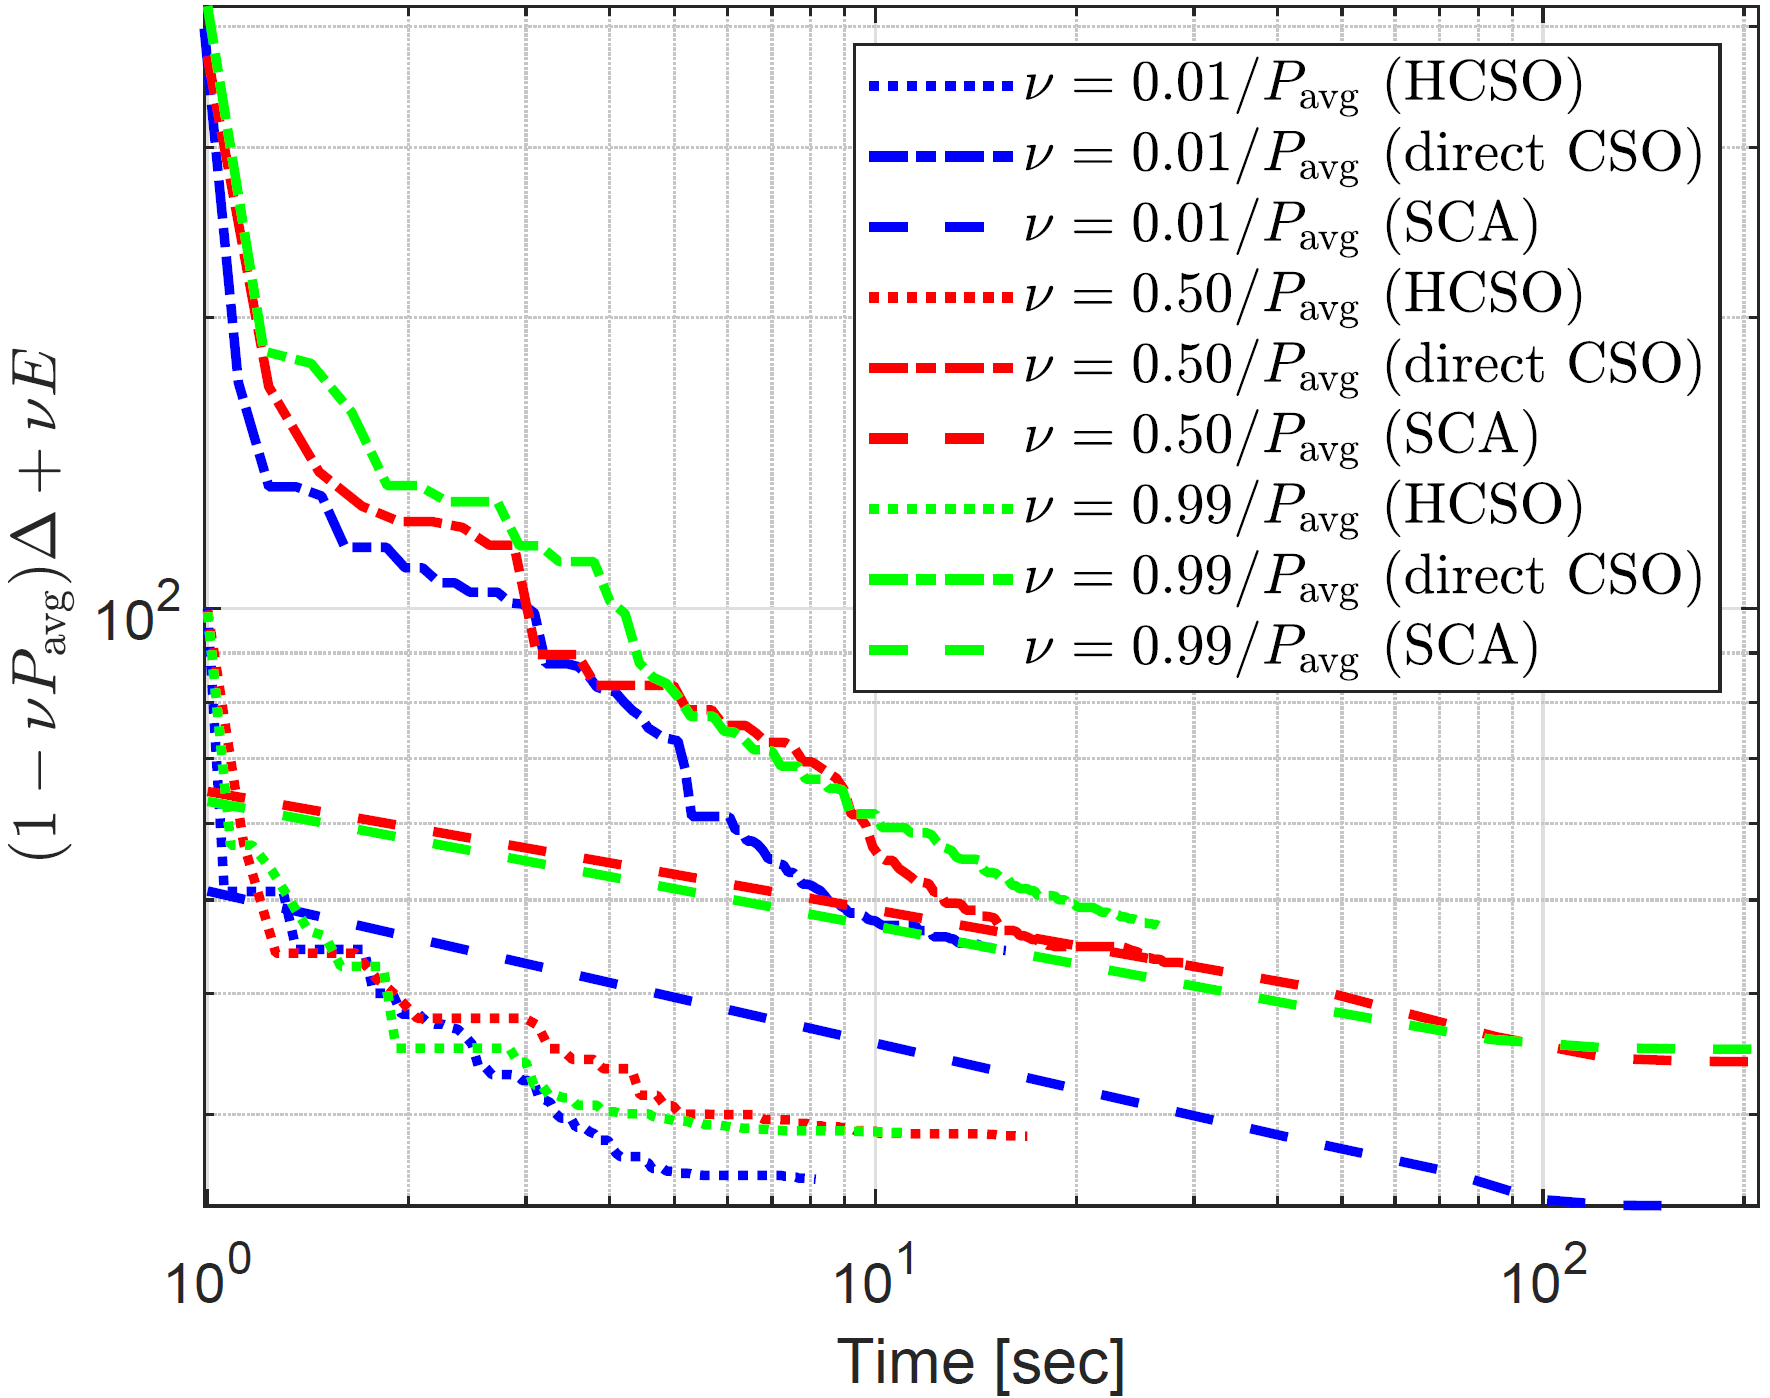
\includegraphics[width=0.815\linewidth]{figs/Convergence.png}
		\caption{Convergence Bench-marking}
		\label{F5}
	\end{subfigure}
	\begin{subfigure}{0.49\textwidth}
  		\centering
  		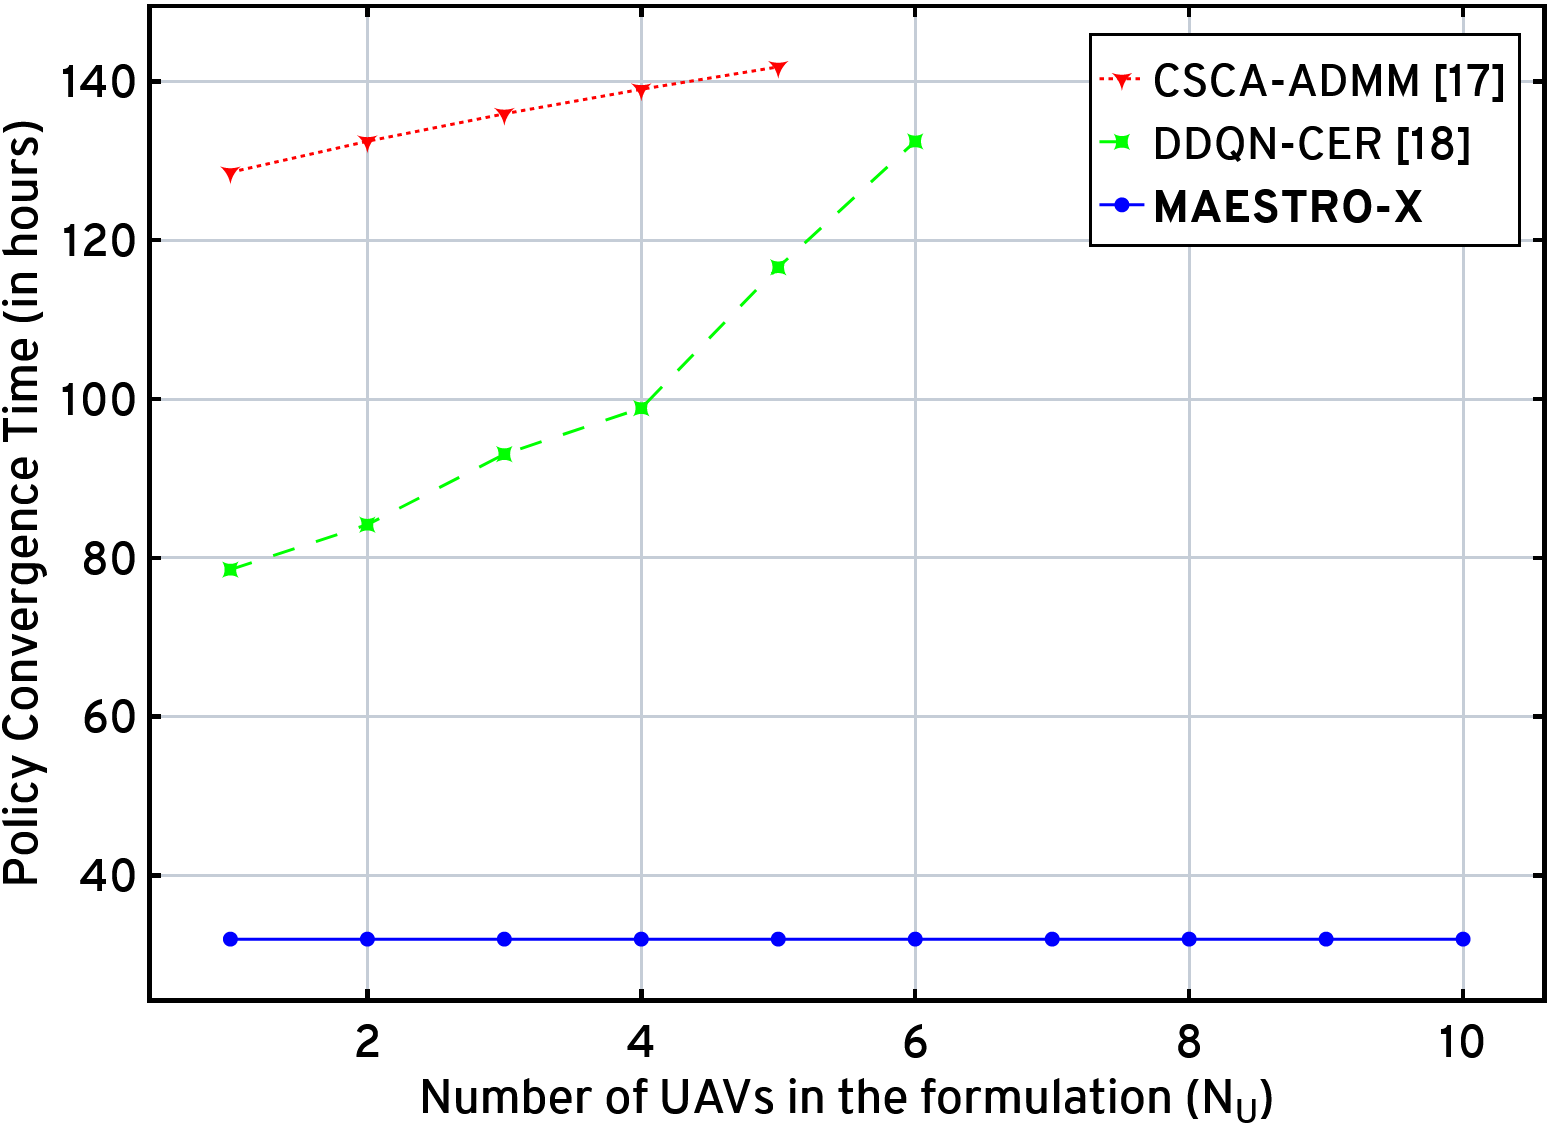
\includegraphics[width=0.9\linewidth]{figs/Complexity.png}
  		\caption{Computation Time Bench-marking}
  		\label{F6}
	\end{subfigure}
	\caption{Convergence bench-marking of HCSO against the CSO and SCA schemes from the state-of-the-art (a); Computational complexity bench-marking of MAESTRO-X against relevant frameworks in the state-of-the-art (b).}
	\vspace{-8mm}
	\label{fig:F5andF6}
\end{figure}

For our evaluations of the optimal \emph{waiting} phase behavior, we fix $P_{\mathrm{avg}}=$ \qty[mode=text]{1.2}{\kilo\watt} and $L=1$ Mb or $100$ Mb. Figures \ref{F7} and \ref{F8} show that the UAV moves to and waits by flying around an optimal radius level ($\approx$95 m from the center) to address two considerations: $1$) to be well-positioned for future transmission requests; $2$) to fly at the power-minimizing velocity so as to reduce UAV energy consumption. Comparing the UAV radial velocities between the $L=1$ Mb and $L=100$ Mb, we observe that, near the cell edge, the UAV radial velocity increases for decreasing data payload, as smaller data packets relaying through the UAV complete transmission faster than large ones---thus the UAV is less likely to spend time following trajectories that place it near the cell edge and can afford the additional power consumption required to fly at high velocities when this is the case.

\begin{figure}[t]
    \begin{subfigure}{0.49\textwidth}
		\centering
		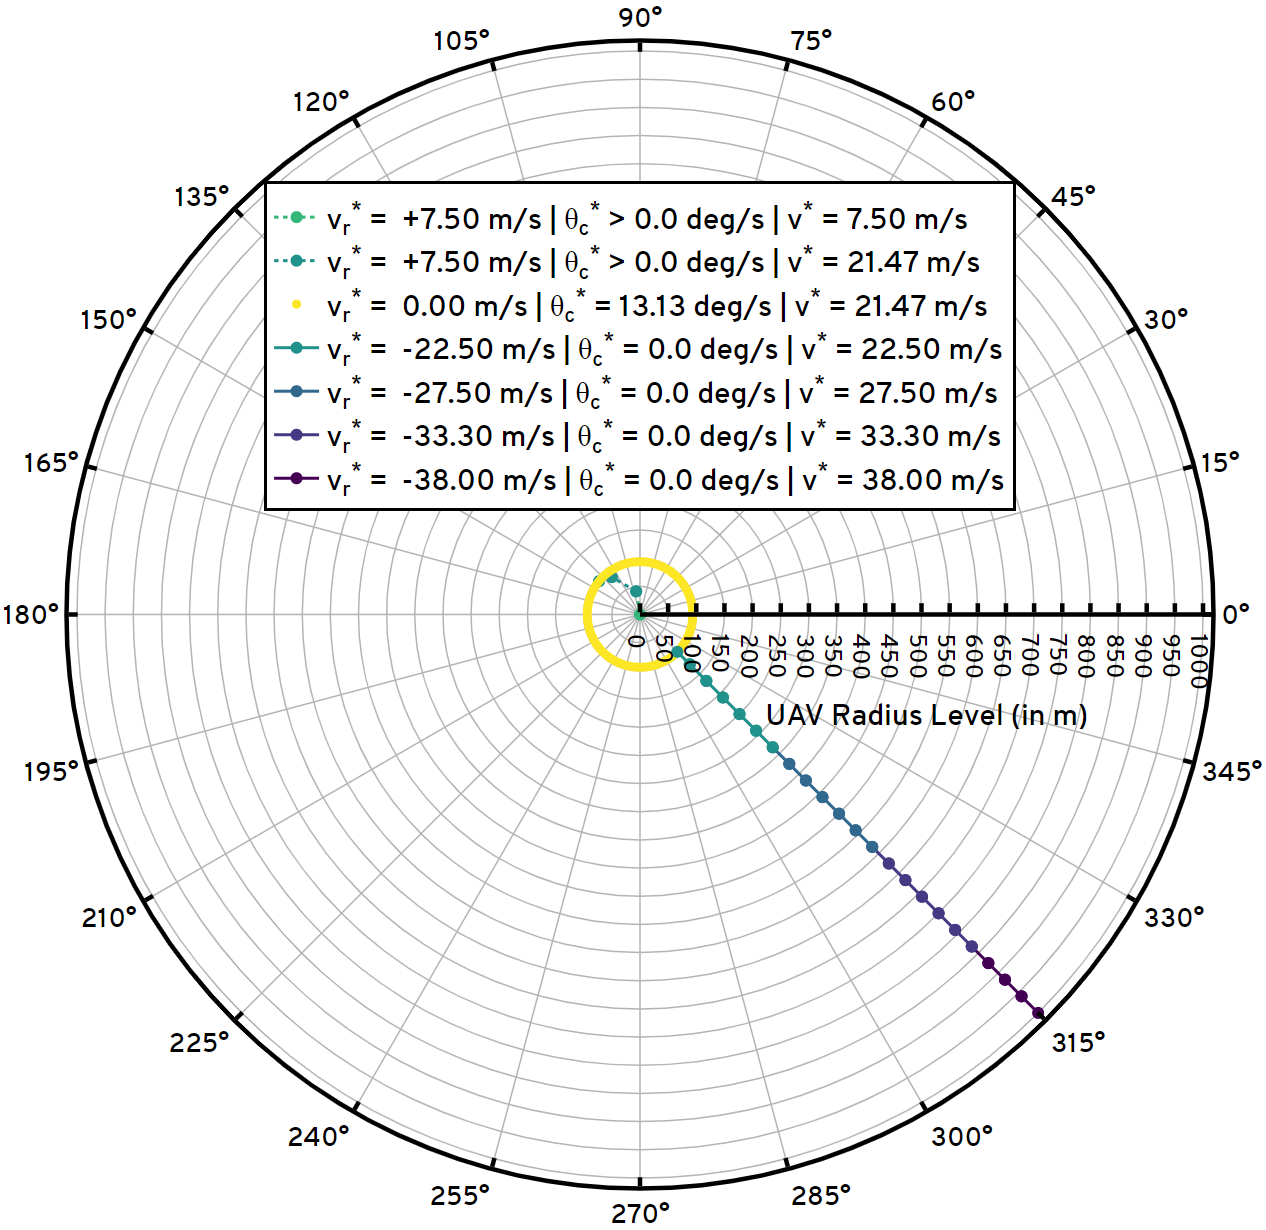
\includegraphics[width=0.9\linewidth]{figs/Wait1.png}
		\caption{$L=1$ Mb}
		\label{F7}
	\end{subfigure}
	\begin{subfigure}{0.49\textwidth}
  		\centering
  		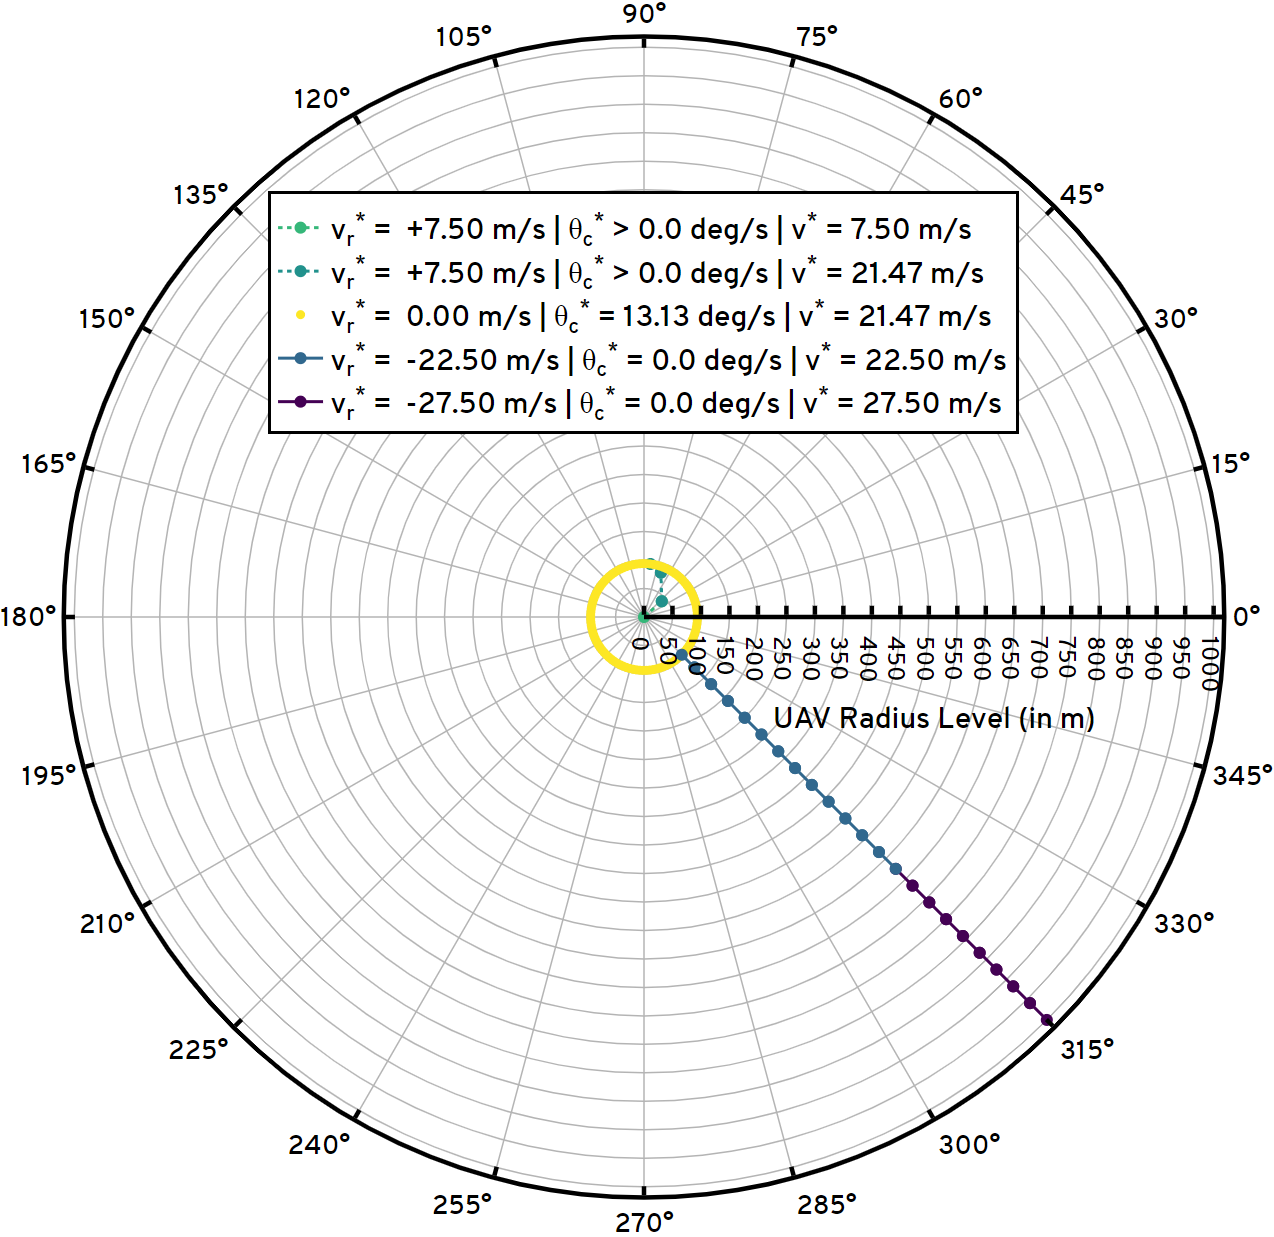
\includegraphics[width=0.9\linewidth]{figs/Wait100.png}
  		\caption{$L=100$ Mb}
  		\label{F8}
	\end{subfigure}
    \caption{Visualizations of MAESTRO's optimal waiting state policy for $L{=}1$ Mb and $L{=}100$ Mb, with $P_{\mathrm{avg}}=$ \qty[mode=text]{1.2}{\kilo\watt} fixed across both evaluations.}
    \vspace{-8mm}
    \label{fig:F7andF8}
\end{figure}

Analyzing optimal decision-making in the \emph{request scheduling} phase vis-à-vis the single-relay specialization of MAESTRO, Fig. \ref{F9} shows which GNs transmit directly to the BS under the optimal policy $\tilde{\mu}$ during these \emph{request scheduling} phases. The target average power is $P_{\mathrm{avg}}=$ \qty[mode=text]{1.2}{\kilo\watt}, and the UAV radius is $r_U=$ \qty[mode=text]{500}{\meter}. One third of the GNs transmit directly to the BS for small data payloads, i.e., $0.1$ Mb, and as the data payload grows larger and larger, the benefit of relaying through the UAV and utilizing its mobility increases, so that the majority of GNs relay through the UAV. Next, in Fig. \ref{F10}, we observe the trajectory of $3$ UAVs in the swarm executed toward serving $3$ different GN transmission requests. \bk{\underline{Re-generating} Fig. \ref{F10} to visualize $2$D trajectories of all $3$ UAVs, each serving a different GN request.}

\begin{figure}
\centering
	\begin{subfigure}{0.49\textwidth}
  		\centering
  		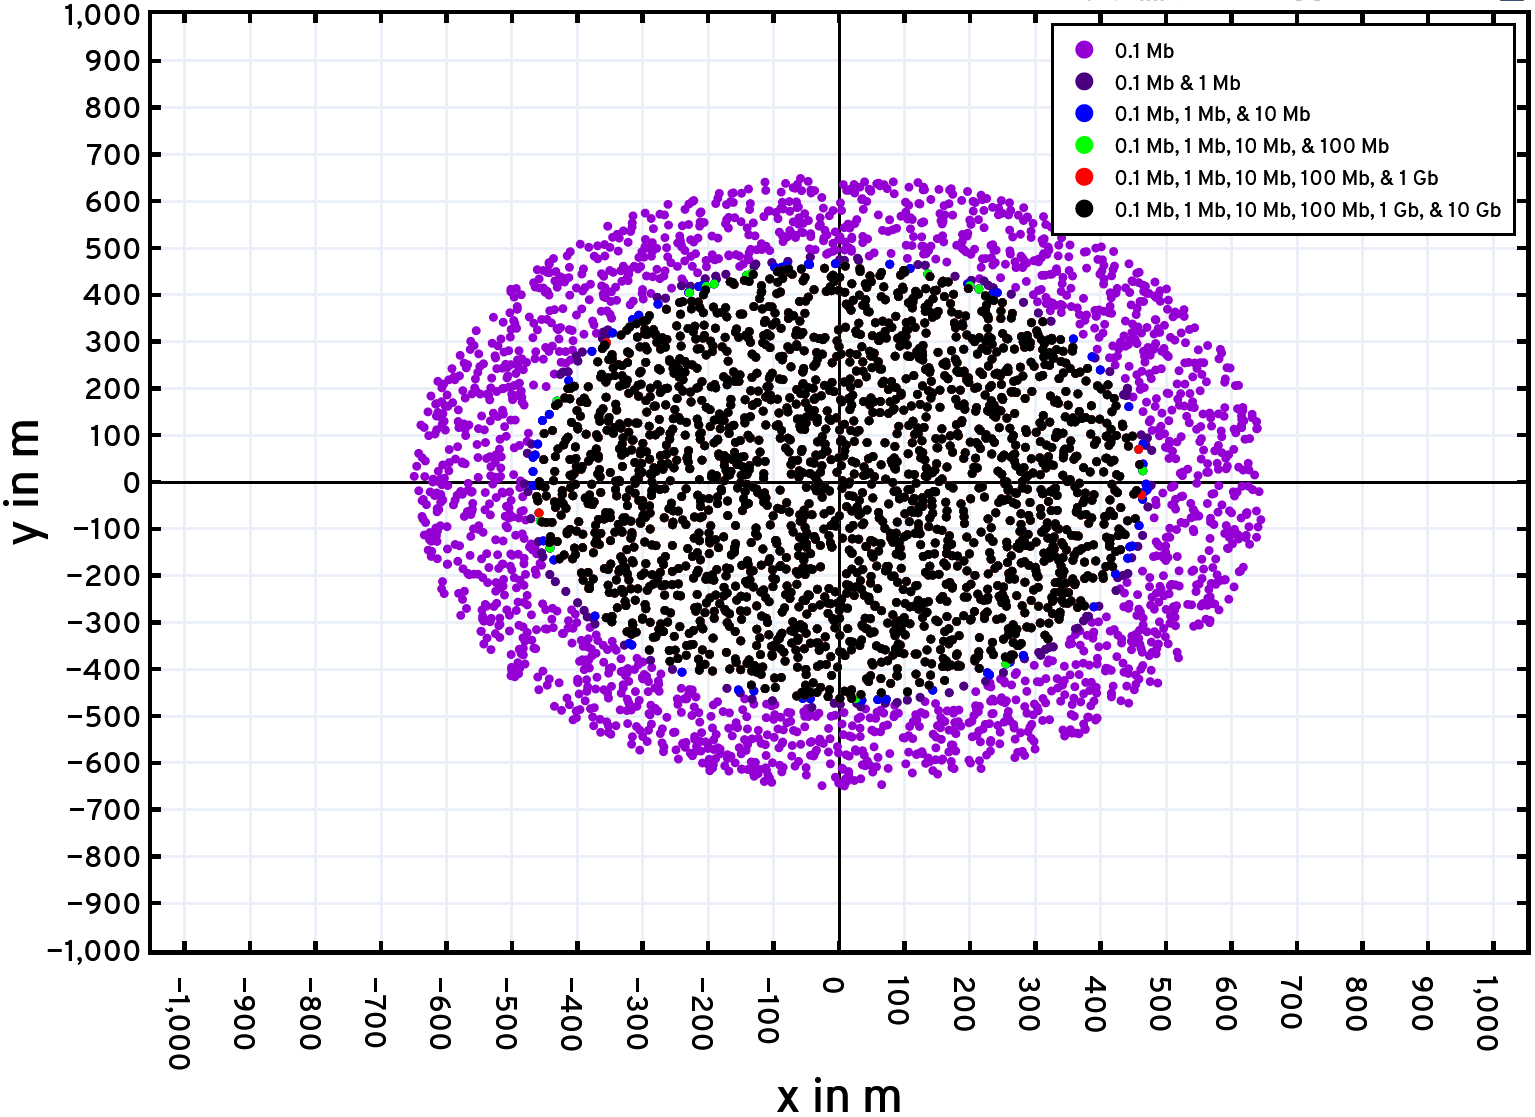
\includegraphics[width=0.9\linewidth]{figs/GN_Distribution.png}
  		\caption{Map of GNs with $\xi{=}0$ for $P_{\mathrm{avg}}=$ \qty[mode=text]{1.2}{\kilo\watt}}
  		\label{F9}
	\end{subfigure}
	\begin{subfigure}{0.49\textwidth}
  		\centering
  		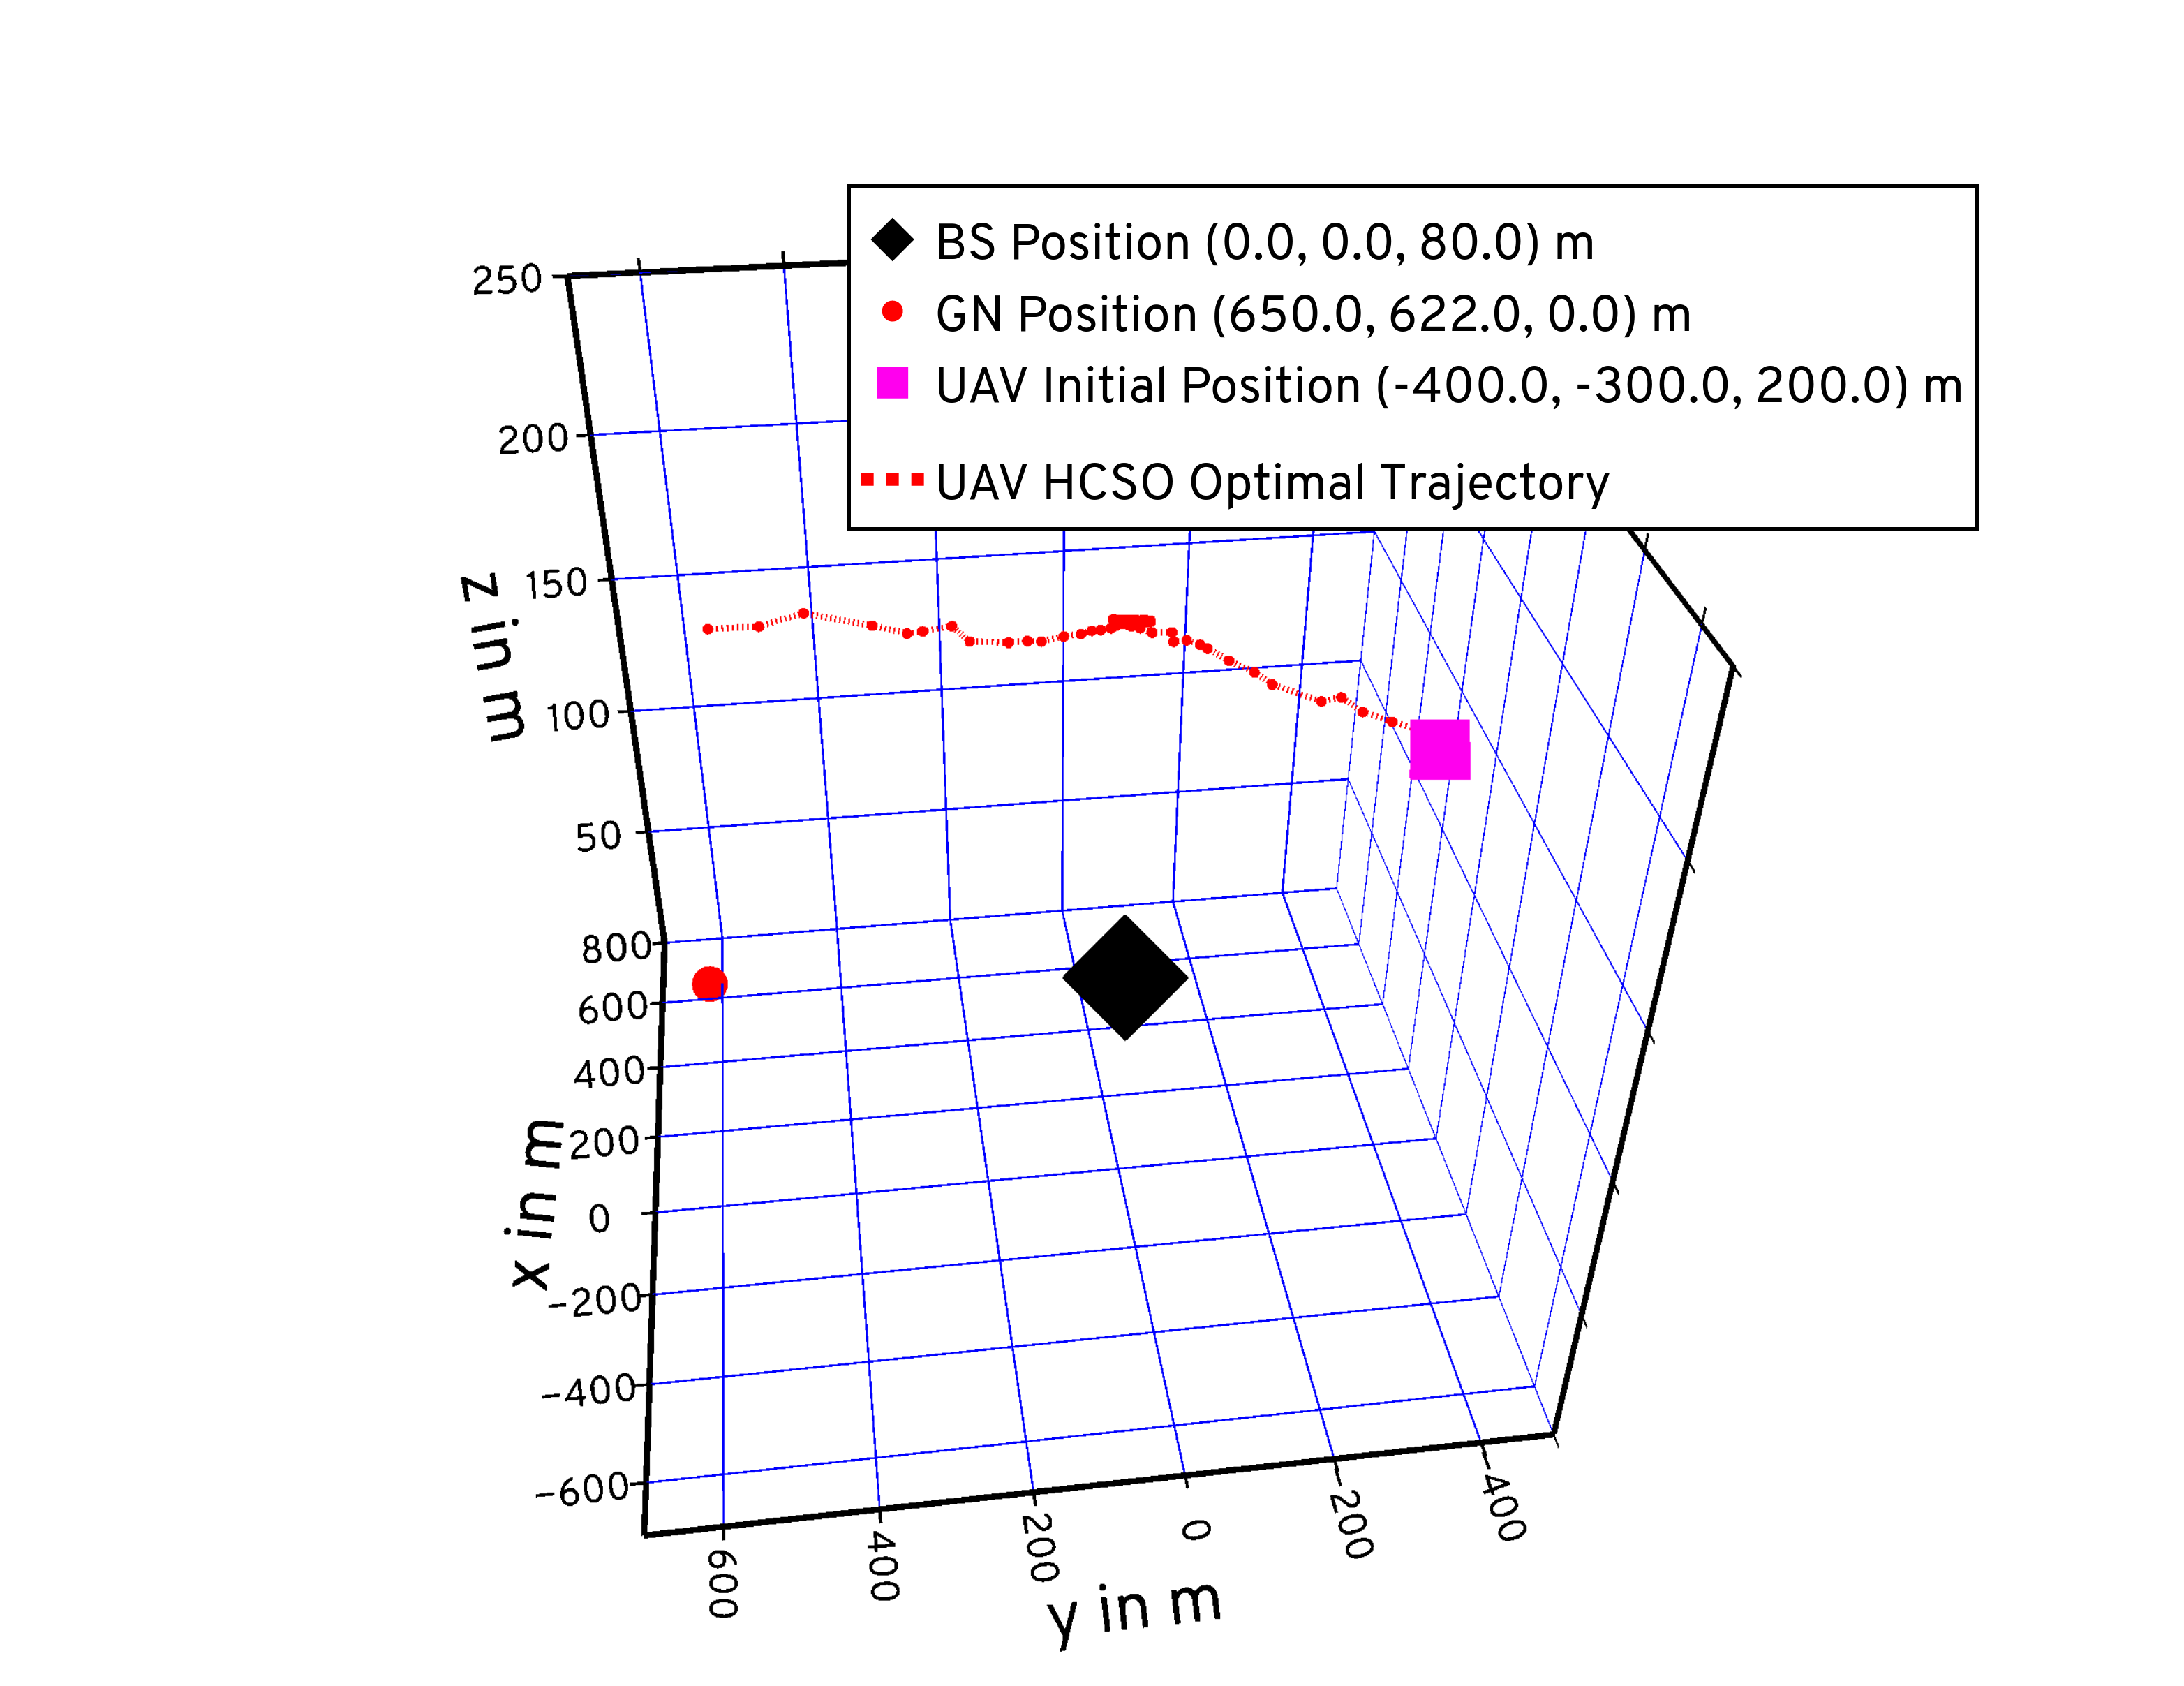
\includegraphics[width=0.9\textwidth]{figs/Trajectory.png}
		\caption{Optimal trajectory for $L{=}10$Mb and $P_{\mathrm{avg}}=$ \qty[mode=text]{1.2}{\kilo\watt}}
		\label{F10}
	\end{subfigure}
\caption{The GNs that are scheduled to be handled by the BS according to MAESTRO's optimal policy in the \emph{communication} states (a); The optimal trajectory of $\text{UAV}_{2}$ under the MAESTRO-X framework, as determined by HCSO, when the active GN request is at $(650,622,0)$ m and $\text{UAV}_{2}$ is initially at $(-400,-300,200)$ m.}
\label{F9andF10}
\vspace{-8mm}
\end{figure}

To analyze the communication delay performance, we simulate over various data payloads and target average power constraints, $P_{\mathrm{avg}}$, to observe a range of behavior. The expected average delay is shown in Figs. \ref{F11} and \ref{F12}. Note that the expected average delay, $\bar{D}_{\tilde\mu}$, is not directly accessible through the value iteration analysis, so we apply the optimal policy $\tilde{\mu}$ in a simulation, sampling a sequence of $10,000$ random transmission requests, in order to obtain it. In Fig. \ref{F11}, we compare the performance of MAESTRO-X with that of different network deployment strategies, for $L=1$ Mb and $L=100$ Mb under varying average per-UAV power constraints: these evaluations are listed below.
\begin{itemize}
    \item M/G/x BS Only: In this deployment, there are no UAV relays supplementing the terrestrial BS in the cell. We analyze the communication delays in this BS-only setting, in addition to queue wait times studies\footnote{All queueing studies in our numerical evaluations are performed via SimPy implementations in Python: M/G/$N_{B}$ for the BS and M/G/$1$ for each UAV.} with $N_{B}=1,\ 5,\ \text{and}\ 10$. Expectedly, we find a significant reduction in the average communication delay experienced by the GNs in the cell, by employing UAVs to relay data traffic. Additionally, as illustrated in the delay histograms, an increase in the number of orthogonal BS channels leads to a considerable increase in the queue wait times.
    \item Static UAVs: In this deployment, we evaluate the delay performance of static UAVs serving as a BS relay for the GNs in the cell. Here, we find that dynamic UAV deployments with optimized trajectories (way-points and velocities) demonstrate lower service delays compared to static deployments---specifically, for a swarm of $3$ UAV relays, with $L=100$ Mb and a per-UAV power consumption of \qty[mode=text]{1.37}{\kilo\watt}, MAESTRO-X services uplink transmission requests from the GNs $20{\times}$ faster than a static deployment of $3$ UAVs positioned equidistant from the cell center.
    \item MAESTRO-$\alpha$: Here, we study a variant of MAESTRO-X, where in addition to the optimal \emph{waiting} and \emph{communication} policy extended from MAESTRO, with spread maximization and conflict resolution, we employ a `Join-Shortest-Queue (JSQ)\footnote{JSQ: The BS queue wait times for a new GN uplink transmission is determined based on the queue (channel) with the smallest number of requests in waiting}' heuristic at the BS to determine the queue wait times during the consensus-driven conflict resolution process in the \emph{request scheduling phase} as opposed to a `Join-Fastest-Queue (JFQ)\footnote{JFQ: The BS queue wait times for a new GN uplink transmission is determined based on the queue (channel) that has the smallest waiting time.}' heuristic in MAESTRO-X. For a swarm with $3$ UAV relays, We observe that a JFQ-scheme at the BS results in $3{\times}$ lower average service delay that a JSQ-scheme.
    \item MAESTRO-$\beta$: Here, we study another variant of MAESTRO-X, where the optimal \emph{waiting} state policy of MAESTRO is replaced with a heuristic in which the UAVs return to the cell center (at $V_{\mathrm{max}}$) immediately after transitioning to the \emph{waiting} state; MAESTRO's optimal \emph{communication} policy is extended with consensus-driven conflict resolution as is the case for MAESTRO-X. We note that, for a swarm of $3$ UAVs, with $L=100$ Mb, this `Return-to-Center (R2C)' \emph{waiting} policy in MAESTRO-$\beta$ as opposed to the optimal \emph{waiting} policy in MAESTRO-X, results in $3{\times}$ worse delay performance.
\end{itemize}

\begin{figure}[t]
    \begin{tabular}{cc}
        \begin{minipage}{0.48\linewidth} 
        	 \centering
             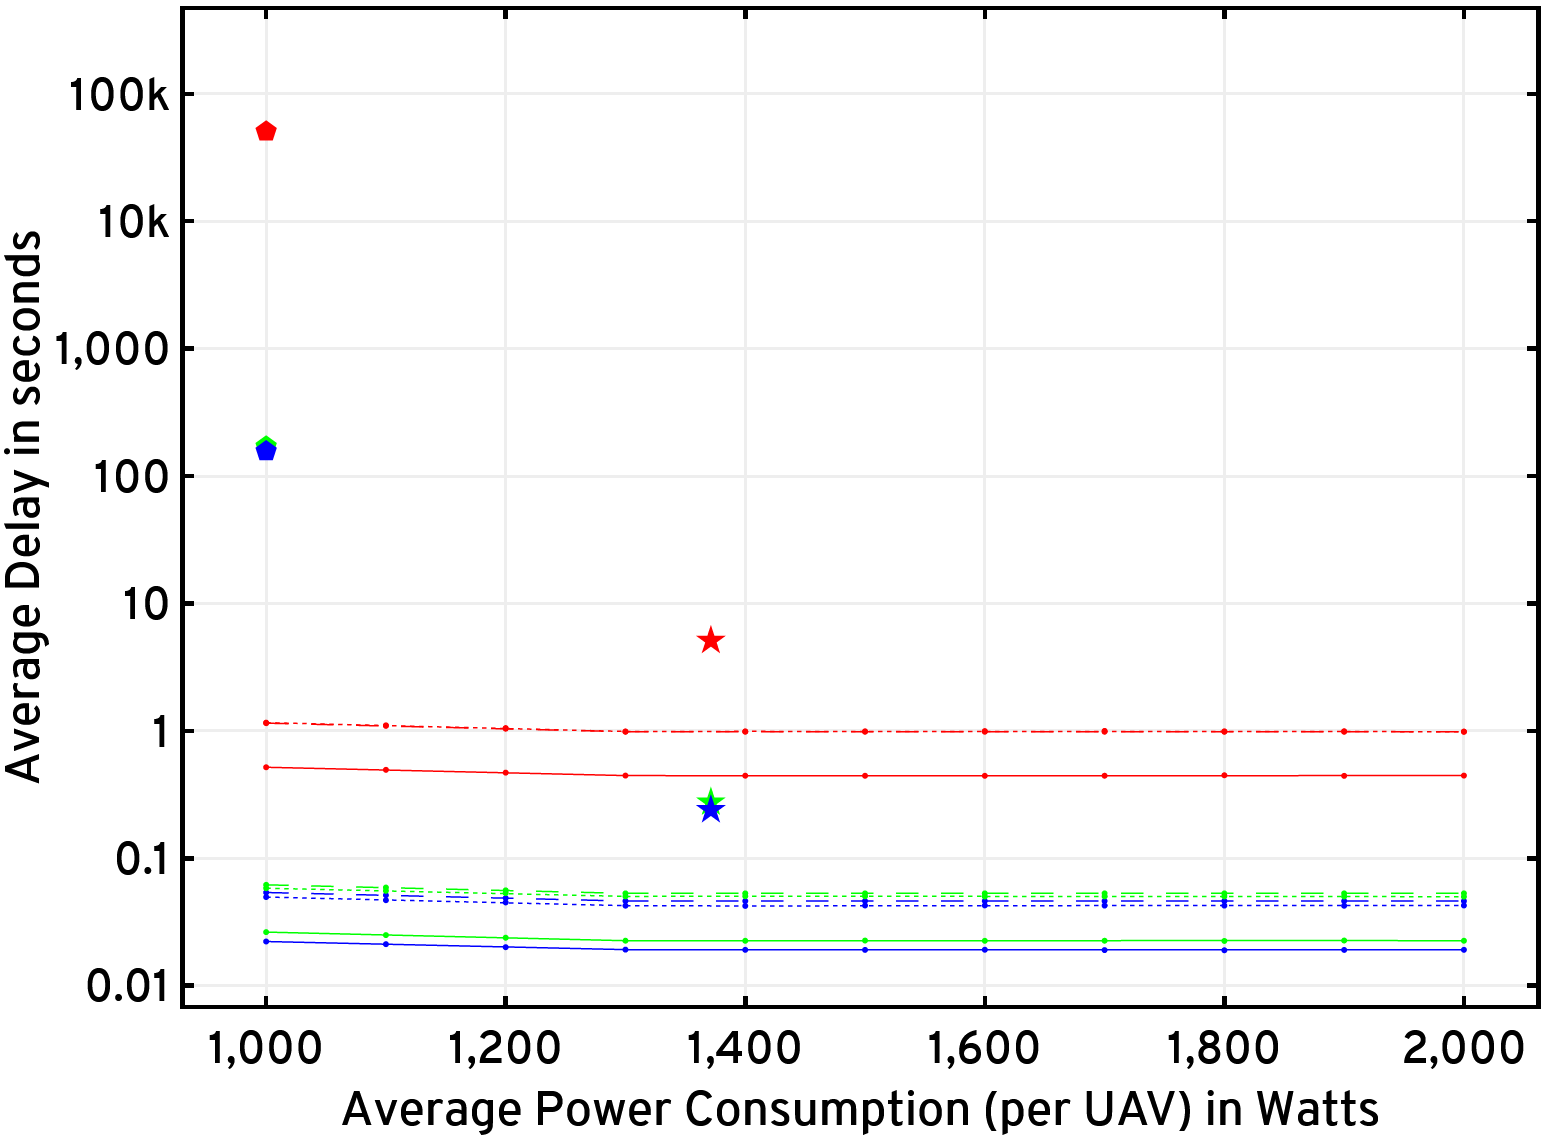
\includegraphics[width=0.9\linewidth]{figs/1Mb_I.png}
             \\ [1.5ex]
             \centering
             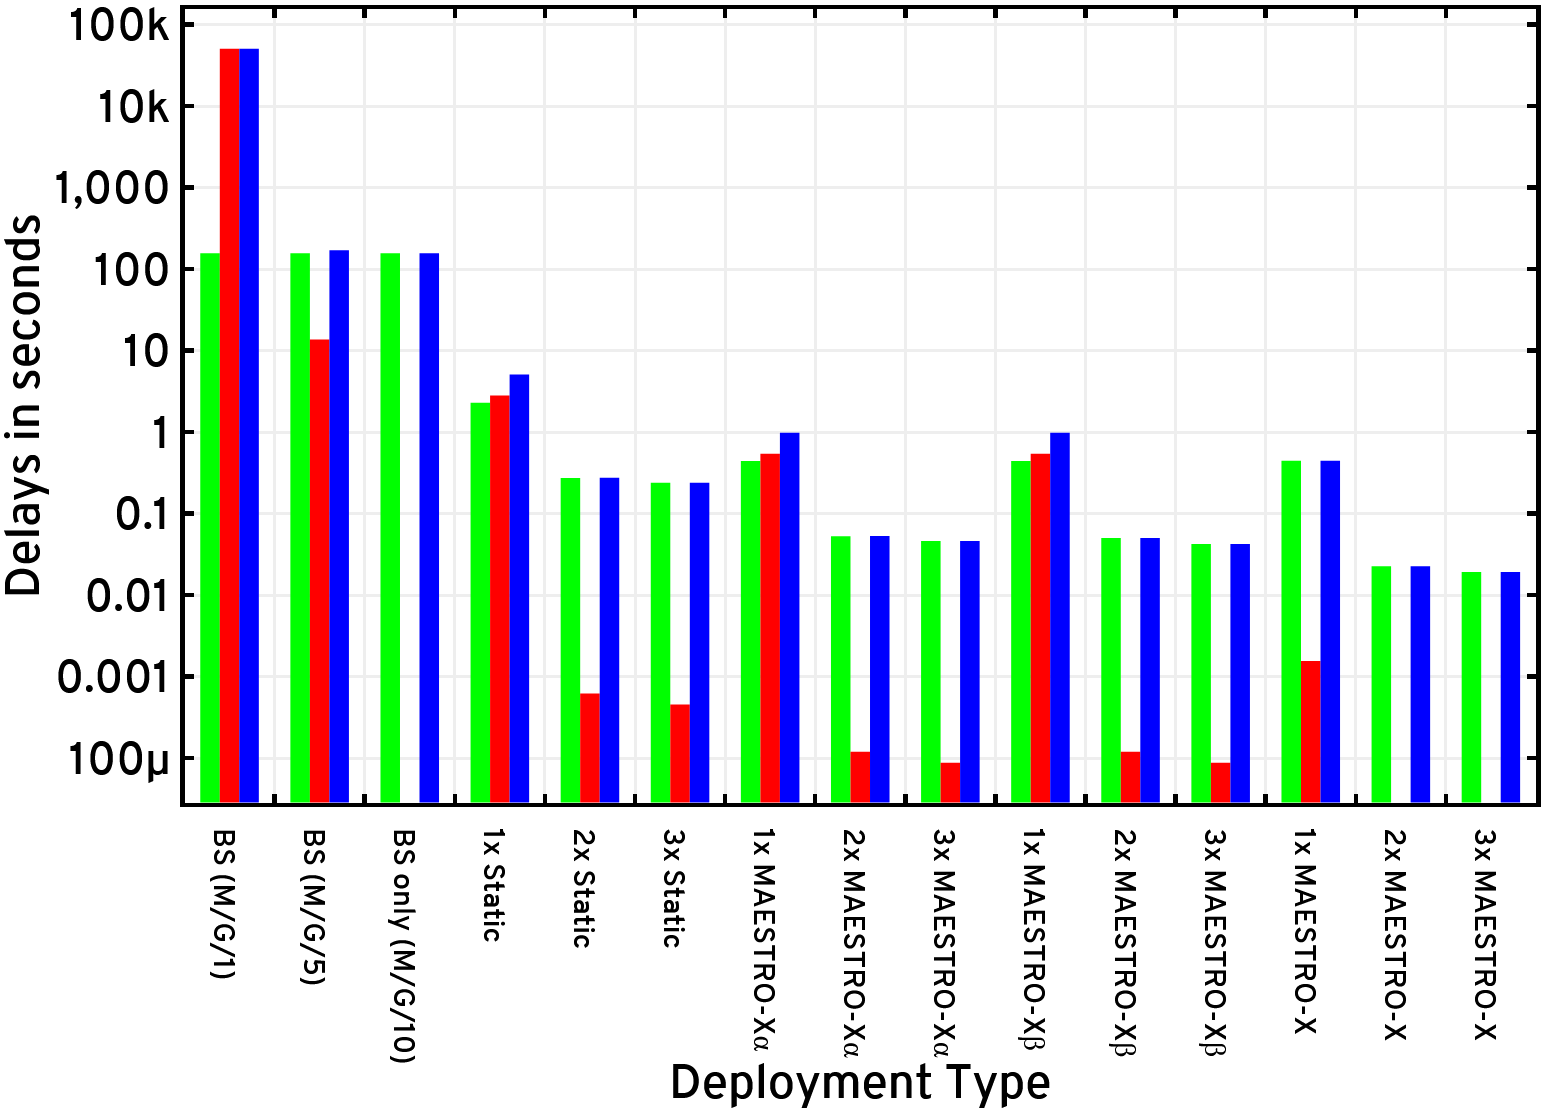
\includegraphics[width=0.9\linewidth]{figs/1Mb_Histogram_I.png}
        \end{minipage}&
        \hspace{-6mm}
        \begin{minipage}{0.48\linewidth} 
        	 \centering
             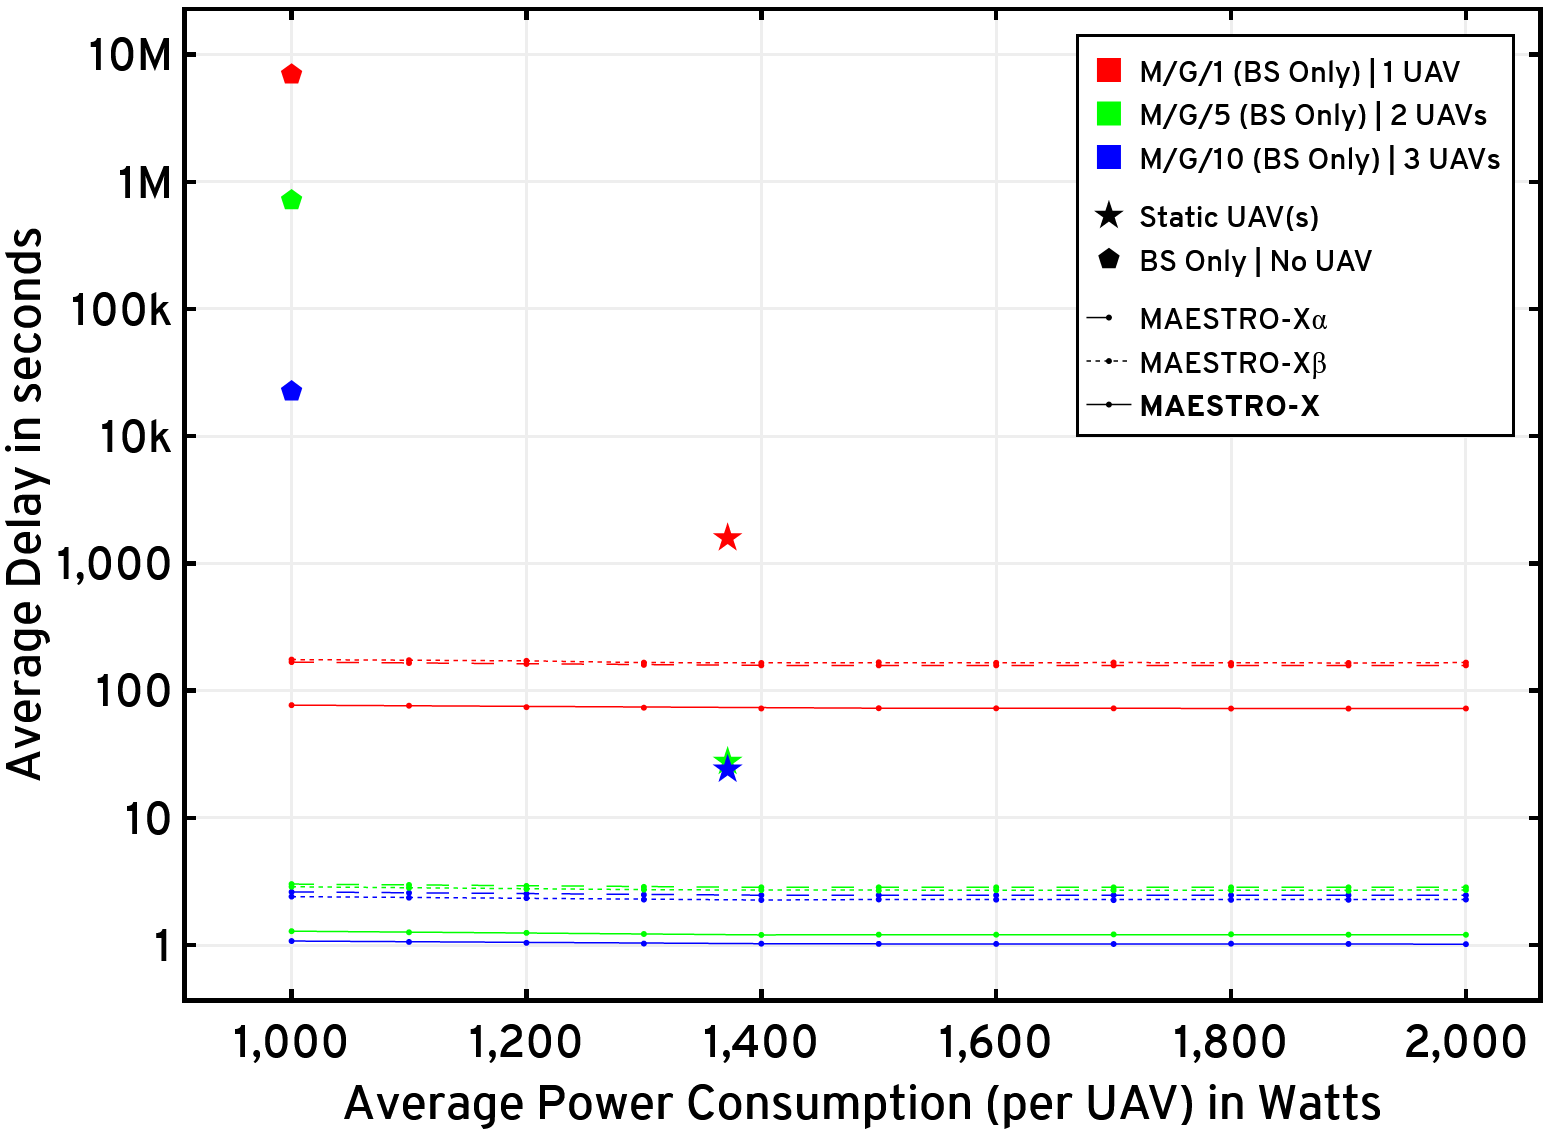
\includegraphics[width=0.9\linewidth]{figs/100Mb_I.png}
             \\ [1.5ex]
             \centering
             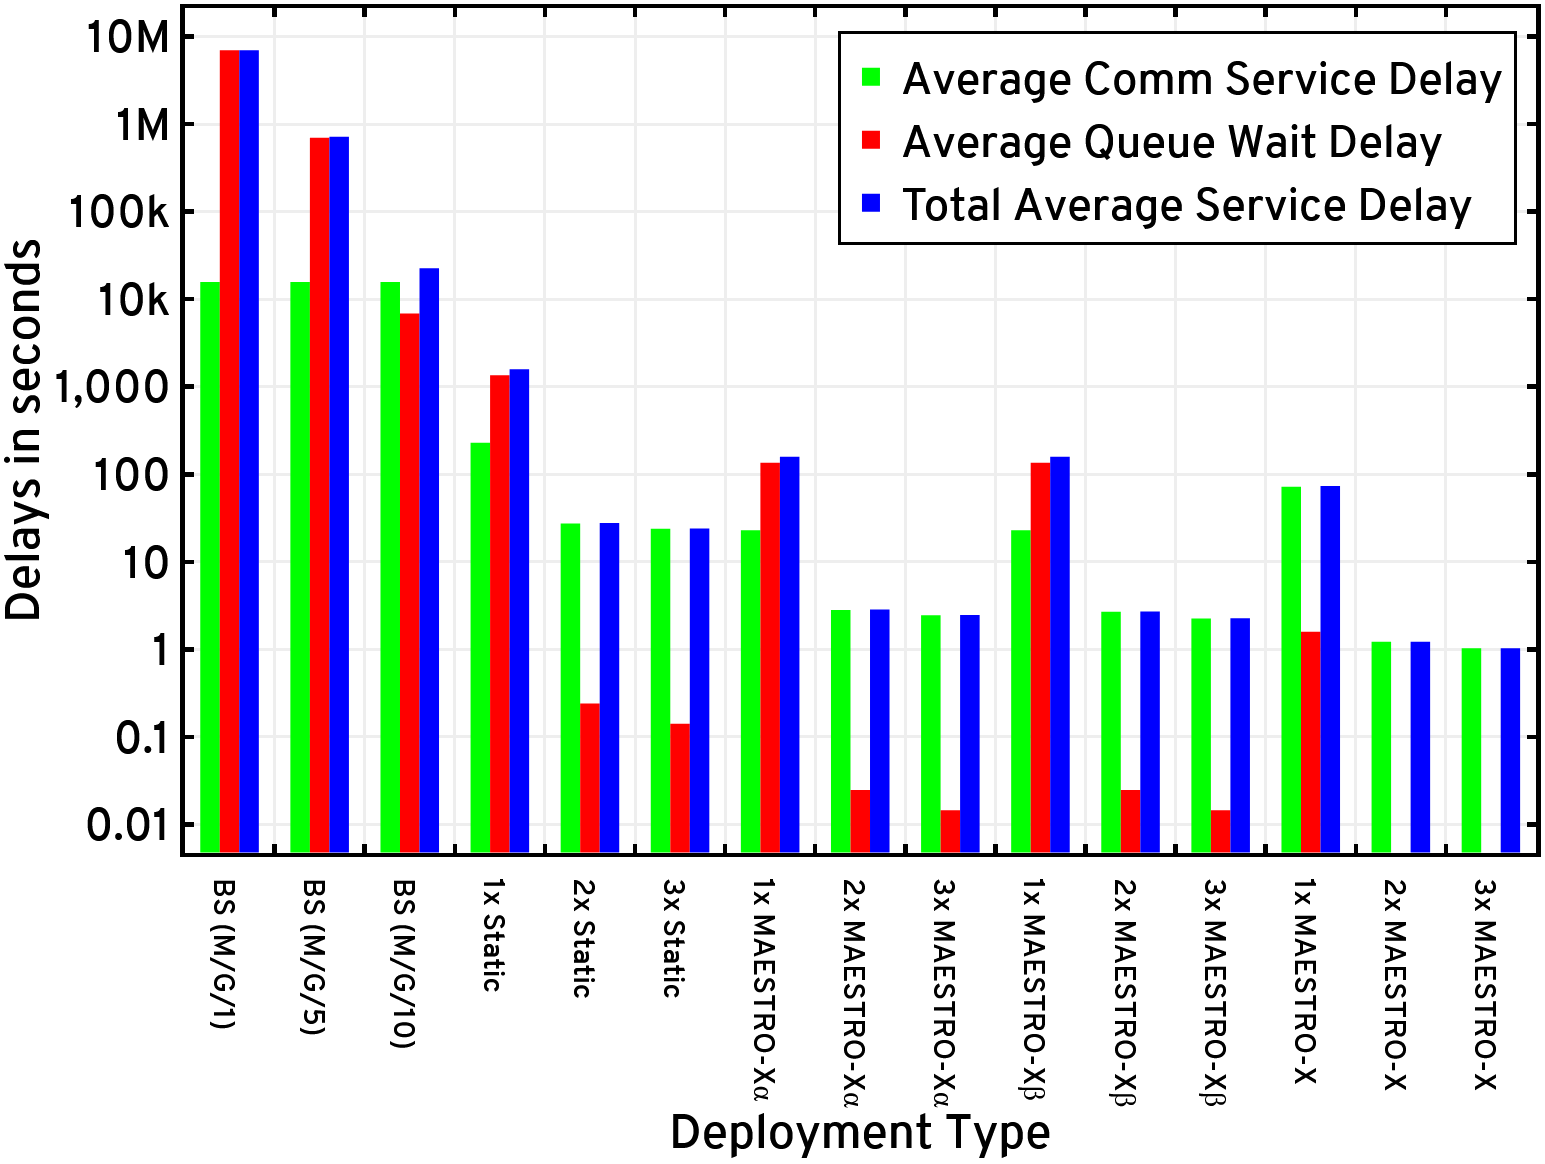
\includegraphics[width=0.9\linewidth]{figs/100Mb_Histogram_I.png}
        \end{minipage}
    \end{tabular}
    \caption{The traces and histograms constituting the average service latencies (communication + queue wait) versus the average power constraint for the proposed MAESTRO-X framework under $L=1$ Mb (left) and $L=100$ Mb (right): Comparisons with custom policy heuristics.}
    \label{F11}
    \vspace{-8mm}
\end{figure}

Continuing with our delay-power analyses of orchestration frameworks for relay swarms, we outline our performance comparisons with relevant schemes in the current literature. These comparisons are depicted in Fig. \ref{F12}. For a swarm of $3$ UAV relays, with uplink transmission requests of size $L=100$ Mb from the GNs in the cell, we observe the following improvements in performance over related schemes in the state-of-the-art, averaged over $10,000$ requests with a traffic arrival rate of $1$ request every \qty[mode=text]{1800}{\second}.
\begin{itemize}
    \item Successive Convex Approximation (SCA) \cite{SCA}: Here, with a CVXPY implementation involving $10^{6}$ iterations and an accuracy of $10^{-6}$, this SCA scheme relays GN requests $6{\times}$ slower than MAESTRO-X.
    \item Constrained Successive Convex Approximation with Alternating Direction Method of Multipliers (CSCA-ADMM) \cite{CSCA-ADMM}: With an ADMM scheme employed within SCA, centered around linearly-coupled equality constraints, the framework proposed in \cite{CSCA-ADMM} involves $50$ worker threads (each with a Split Conic Solver optimizer, $10^{6}$ iterations, and an accuracy of $10^{-6}$) solving the optimization problem within an SCA wrapper; MAESTRO-X demonstrates $10{\times}$ better QoS performance vis-à-vis service latencies, for an average per-UAV power constraint of \qty[mode=text]{1.2}{\kilo\watt}.
    \item Double Deep Q-Network with Combined Experiential Replay (DDQN-CER) \cite{DDQN}: This model-free approach revolving around a decentralized POMDP\footnote{Partially Observable Markov Decision Processes} formulation, with an average per-UAV power constraint of \qty[mode=text]{1.1}{\kilo\watt} demonstrates $4{\times}$ slower request service times relative to MAESTRO-X.
\end{itemize}

\begin{figure}[t]
    \begin{tabular}{cc}
        \begin{minipage}{0.48\linewidth} 
        	 \centering
             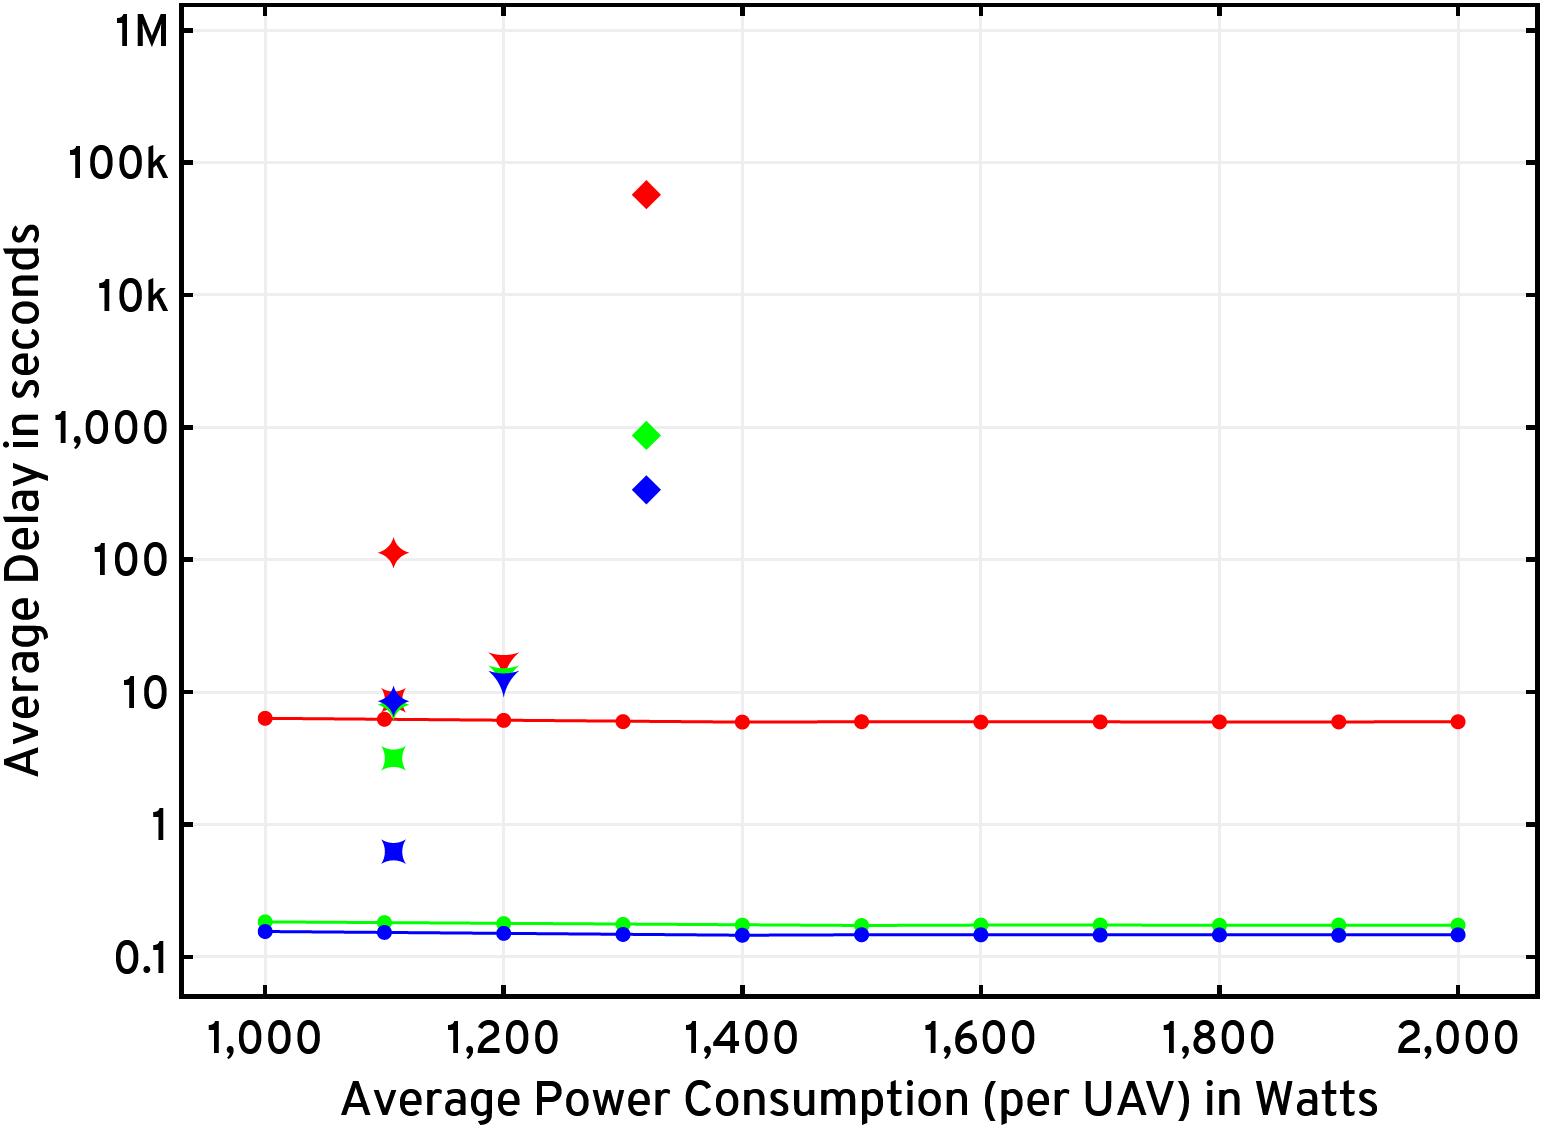
\includegraphics[width=0.9\linewidth]{figs/1Mb_II.png}
             \\ [1.5ex]
             \centering
             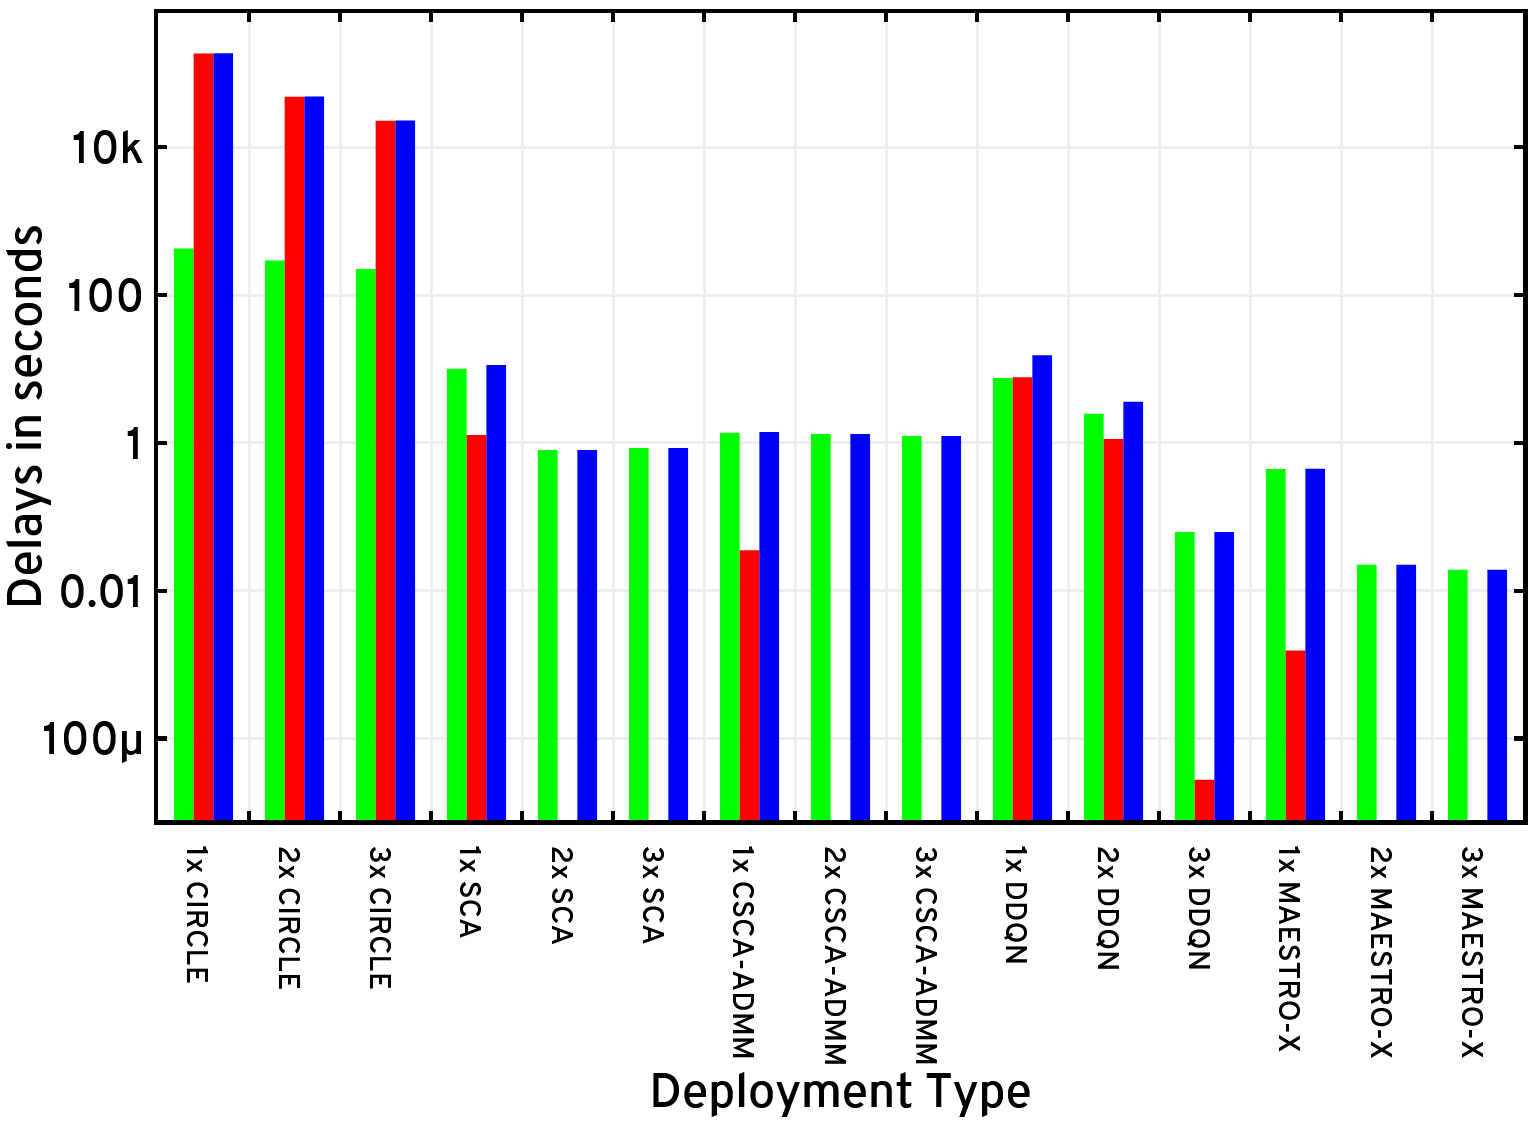
\includegraphics[width=0.9\linewidth]{figs/1Mb_Histogram_II.png}
        \end{minipage}&
        \hspace{-6mm}
        \begin{minipage}{0.48\linewidth} 
        	 \centering
             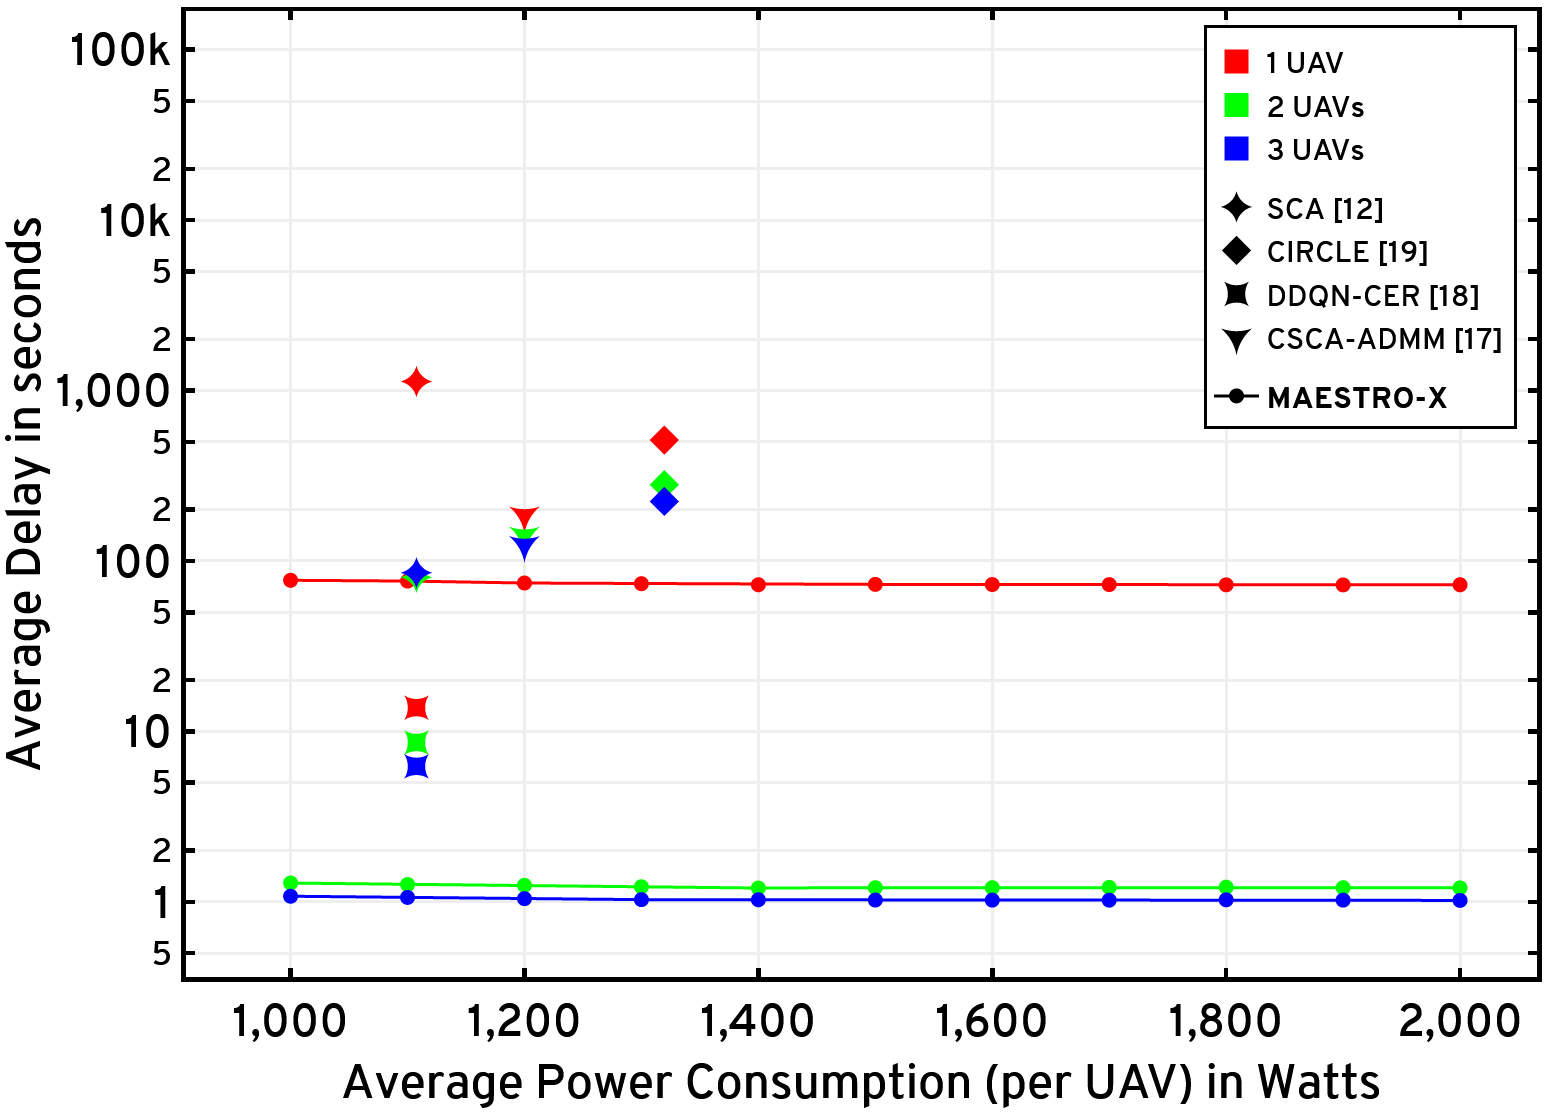
\includegraphics[width=0.9\linewidth]{figs/100Mb_II.png}
             \\ [1.5ex]
             \centering
             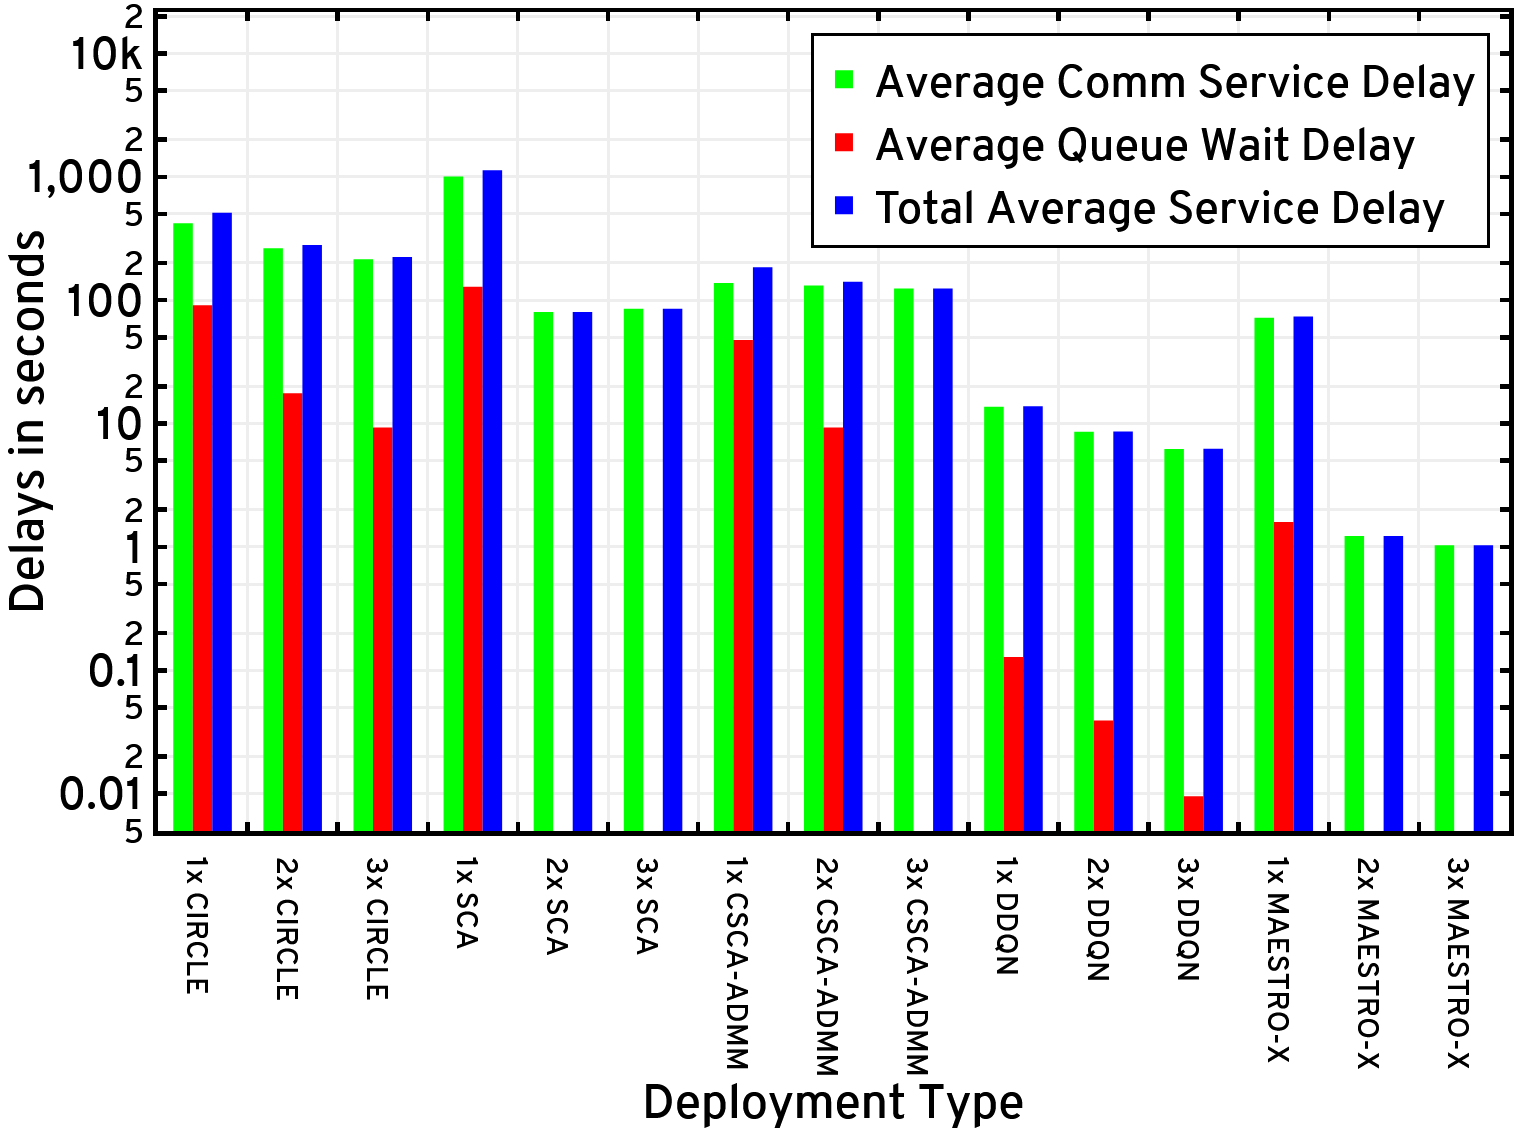
\includegraphics[width=0.9\linewidth]{figs/100Mb_Histogram_II.png}
        \end{minipage}
    \end{tabular}
    \caption{The traces and histograms constituting the average service latencies (communication + queue wait) versus the average power constraint for the proposed MAESTRO-X framework under $L=1$ Mb (left) and $L=100$ Mb (right): Comparisons with relevant schemes in the state-of-the-art.}
    \label{F12}
    \vspace{-8mm}
\end{figure}
\vspace{-4mm}

\section{MAESTRO-X on AERPAW: Feasibility Analyses}\label{S7}
\vspace{-2mm}

\bk{\underline{Emulations underway}: The emulations of MAESTRO and MAESTRO-X are in progress on the EVMs of the AERPAW testbed. Upon their completion, I will add a couple of images from the QGControl trajectory executions and talk about a few metrics from the traffic logs.}


\section{Conclusions}\label{S8}
\vspace{-2mm}

In this paper, we propose MAESTRO-X: a framework for the decentralized orchestration of a swarm of rotary-wing UAV relays in hybrid wireless networks, augmenting the coverage and service capabilities of a terrestrial BS. First, we specialize our system model to single-UAV deployments and design the optimal request scheduling and trajectory optimization policy under an SMDP formulation (via value iteration and HCSO). Next, we extend this single-relay policy to distributed deployments of two or more UAVs by supplementing the policy with multi-UAV coordination heuristics and M/G/x queueing analyses, and replicate this augmented policy across the swarm. Numerical evaluations demonstrate that MAESTRO-X delivers significant performance improvements to `BS-only' and 'Static UAV' deployments; furthermore, MAESTRO-X outperforms popular Q-learning and successive convex approximation strategies in the existing literature. Finally, we demonstrate the integration and implementation viability of MAESTRO-X on the NSF AERPAW platform through QGroundControl based emulations.
\vspace{-4mm}


\appendices

%%%
% \section*{Appendix A: Convexity of $-\ln f(z)-\ln Q_{1}\left(a_1, a_2z\right)$}\label{AA}
% \vspace{-2mm}

% To show this, note that $Q_{1}\left(a_1, y\right)$ is log-concave in $y{\geq}0$ \cite{MarcumConcavity},
% so that $-\ln Q_{1}\left(a_1, a_2z\right)$ is convex in $z\geq 0$. We now show that $[-\ln f(z)]$ is convex, i.e.,  $\frac{\mathrm d^2}{\mathrm dz^2}[-\ln f(z)]{\geq}0,\forall z{\geq}0$. We have
% $$
% \frac{\mathrm d^2}{\mathrm dz^2}[-\ln f(z)]\propto
% 2z^2
% +\left(z^2-2\right)\ln\left(1+z^2/2\right)\triangleq h(z).
% $$
% $h(z){\geq}0$ holds trivially for $z{\geq}\sqrt{2}$, and it can be shown to hold for $z\leq\sqrt{2}$ by using $\ln(1+x)\leq x$.
% \vspace{-4mm}
%%%

\section*{Appendix A: Proof of Lemma \ref{lem:UpLowB}}\label{AA}
\vspace{-2mm}

Consider $\bar{W}_{\mu}$ in \eqref{eq:BarDefs}. If $\xi_u{=}1$, then additional requests received during the UAV relay phase are served directly by the BS, with delay $\frac{L}{\bar{R}_{GB}(r)}$ for a GN in position $(r,\theta)$. Hence,
the expected average communication delay to serve these additional requests is
$\mathbb{E}[\Delta_{u,i}^{(bs)}]{=}\bar{D}_{BS}$, yielding
\begin{align}\label{eq:WBar}
    \bar{W}_{\mu} = \lim\limits_{t \rightarrow \infty} \mathbb{E}_{\mu} \left[ \frac{1}{M_t} \sum_{u = 1}^{M_t }[\Delta_u^{(s)}+\xi_u N_u\bar{D}_{BS}] \right]
    =
    \bar{D}_{BS}(\bar{N}_{\mu} -1)
    + \bar{W}_{\mu}^{(s)},
\end{align}
where the second step uses the definition of $\bar{N}_{\mu}$ in \eqref{eq:BarDefs}. Then, it follows that
\begin{align}\label{fdgh}
    &\bar{D}_{\mu}
    =\frac{\bar{W}_{\mu}}{\bar{N}_{\mu}}
    =\frac{1}{\bar N_{\mu}}\bar{W}_{\mu}^{(s)}
    +\left(1-\frac{1}{\bar N_{\mu}}\right)\bar{D}_{BS}.
\end{align}
Let $\mu_{BS}$ be the policy such that the UAV flies at the power-minimizing velocity $V_{\mathrm{min}}$, and all requests are served by the BS. This policy is feasible (it uses minimum power) and its average delay is $\bar{D}_{\mu_{BS}}{=}\bar{D}_{BS}$, since all requests are served directly by the BS. Therefore, under the optimal policy we must have $\bar{D}_{\mu}^{*}{\leq}\bar{D}_{\mu_{BS}}{=}\bar{D}_{BS}$. Using \eqref{fdgh} and the fact that $\bar{N}_{\mu}{\geq}1$, this implies that $\bar{W}_{\mu^{*}}^{(s)}{\leq}\bar{D}_{BS}$. Let $\mu$ be any policy that satisfies $\bar{W}_{\mu}^{(s)}{\leq}\bar{D}_{BS}$ (note that any other policy is sub-optimal). Under such policy, \eqref{fdgh} along with $\bar{N}_{\mu}{\geq}1$, implies $\bar{W}_{\mu}^{(s)}{\leq}\bar{D}_{\mu}{\leq}\bar{D}_{BS}$.

Moreover, if $\xi_{u}{=}1$, then $N_{u}$ requests are received during the \emph{UAV relay} phase of duration $\Delta_u^{(s)}$; since these requests are received with a rate $\Lambda$, we find that
$\mathbb{E}[N_{u}|\Delta_u^{(s)}]{=}\Delta_u^{(s)}\Lambda$, so that using the bound $\xi_{u}{\leq}1$, we can express
\begin{align}\label{eq:NBar}
	\bar{N}_{\mu} = \lim_{t \rightarrow \infty} \mathbb{E}_{\mu} \Bigg[ \frac{1}{M_t} \sum_{u = 1}^{M_t }(1+\xi_u\Delta_u^{(s)}\Lambda)\Bigg]
    \leq 1+\Lambda\bar{W}_{\mu}^{(s)},
\end{align}
with strict equality if the UAV always serves requests. Under any policy $\mu$ such that $\bar{W}_{\mu}^{(s)}{\leq}\bar{D}_{BS}$, we can then bound as in \eqref{eq:ULBound}, where the second inequality follows from $\bar{W}_{\mu}^{(s)}{\leq}\bar{D}_{BS}$.
\vspace{-4mm}

\section*{Appendix B: Evaluation of $\pi_{\mathrm{comm}}$}\label{AB}
\vspace{-2mm}

\begin{lemma}\label{lem:SSComm}
	Let $\pi_{\mathrm{comm}}{=}\int_{\mathcal{S}_{\mathrm{comm}}}\!\!\!\!\!\Pi_{\mu}(s)\mathrm{d}s$ and $\pi_{\mathrm{wait}}{=}1{-}\pi_{\mathrm{comm}}$ be the steady-state probabilities that the UAV is in the waiting and communication phases in the SMDP, respectively. We have that
    \begin{align}\label{eq:SSCommResult}
    	\pi_{\mathrm{wait}} = \frac{1}{2-e^{-\Lambda \Delta_0}}, \; \pi_{\mathrm{comm}} = \frac{1-e^{-\Lambda \Delta_0}}{2-e^{-\Lambda \Delta_0}}.
    \end{align}
\end{lemma}

\begin{proof}
Let $p_{ww}{=}e^{-\Lambda\Delta_{0}}$ and $p_{cw}{=}1$ 
be the probabilities of remaining in the waiting phase ($ww$; if no request is received, the SMDP remains in the waiting state) and of moving from a communication to a waiting state ($cw$; 
a waiting state always follows a communication state) in one SMDP state transition, respectively. Therefore, $\pi_{\mathrm{wait}}$ and $\pi_{\mathrm{comm}}$ satisfy the stationary equations
\begin{align}
    \begin{cases}
        \pi_{\mathrm{wait}} = \pi_{\mathrm{wait}}p_{ww} + \pi_{\mathrm{comm}}p_{cw} \nonumber
        =e^{-\Lambda \Delta_0}\pi_{\mathrm{wait}} + \pi_{\mathrm{comm}},
        \\
        \pi_{\mathrm{comm}} = \pi_{\mathrm{wait}}(1-p_{ww}) + \pi_{\mathrm{comm}}(1-p_{cw})
        =(1-e^{-\Lambda \Delta_0})\pi_{\mathrm{wait}},\text{ and}\nonumber \\
        \pi_{\mathrm{wait}} + \pi_{\mathrm{comm}} = 1;
    \end{cases}
\end{align}
whose solution is given in the statement of the lemma.
\end{proof}
\vspace{-4mm}


\bibliographystyle{IEEEtran}
\bibliography{IEEEabrv,main} 


\end{document}